\documentclass[a4paper,11pt,fleqn,dvipsnames,twoside,openright]{memoir} 	

%%%% PACKAGES %%%%
% ¤¤ Encoding and language ¤¤ %
\usepackage[utf8x]{inputenc}				
\usepackage[UKenglish]{babel}				
\usepackage[T1]{fontenc}				
\usepackage{ragged2e,anyfontsize}		
\usepackage{fixltx2e}

% ¤¤ Figures and tables (floats) ¤¤ %
\usepackage{graphicx} 					
\usepackage{multirow}                
\usepackage{multicol}         	       
\usepackage{rotating}					
\usepackage{colortbl} 					
\usepackage[table]{xcolor}						
\usepackage{flafter}					
\let\newfloat\relax 					
\usepackage{float}		
\usepackage{longtable}	
\usepackage{etoolbox}

% ¤¤ Math ¤¤ %
\usepackage{amsmath,amssymb,stmaryrd} 	
\usepackage{mathtools}					
\usepackage{textcomp}                 	
\usepackage{rsphrase}				
\usepackage[version=3]{mhchem} 			
\usepackage{siunitx}					

% ¤¤ References and sources ¤¤ %
\usepackage[english]{varioref}			
\usepackage{natbib}              			

% ¤¤ Misc. ¤¤ %
\usepackage{listings}
\usepackage{color}
\usepackage{courier}
\usepackage{dirtree}
%\usepackage{lipsum}						
\usepackage[shortlabels]{enumitem}		
\usepackage{pdfpages}					
\pdfoptionpdfminorversion=6				
\pretolerance=2500 			

\usepackage[footnote,draft,english,silent,nomargin]{fixme}		
\usepackage{lastpage}

%%%% CUSTOM SETTINGS %%%%
% ¤¤ Margins ¤¤ %
\setlrmarginsandblock{3.5cm}{2.5cm}{*}	
\setulmarginsandblock{2.5cm}{3.0cm}{*}	
\checkandfixthelayout 					

% ¤¤ Formatting ¤¤ %
\setlength{\parindent}{0mm}           	
\setlength{\parskip}{3mm}          		
\linespread{1,1}					

% ¤¤ Literature list ¤¤ %
\bibpunct[,]{[}{]}{;}{a}{,}{,} 
\bibliographystyle{plainnat}	

% ¤¤ Table of contents ¤¤ %
\setsecnumdepth{subsection}		 		
\maxsecnumdepth{subsection}				
\settocdepth{section} 				

% ¤¤ Lists ¤¤ %
\setlist{
  topsep=0pt,							
  itemsep=-1ex,							
} 

\newcommand*\Hide{%
\titleformat{\chapter}[display]
  {}{}{0pt}{\Huge}
\titleformat{\part}
  {}{}{0pt}{}
}

% ¤¤ Visual references ¤¤ %
\usepackage[colorlinks]{hyperref}		
\hypersetup{colorlinks = true,	
    linkcolor = black,
    citecolor = black,
    urlcolor = black
}

% ¤¤ Caption layout ¤¤ %
\captionnamefont{\small\bfseries\itshape}	
\captiontitlefont{\small}				
\captiondelim{. }						
\hangcaption							
\captionwidth{\linewidth}				
\setlength{\belowcaptionskip}{0pt}		
		
% ¤¤ Listings layout ¤¤ %
\definecolor{commentGreen}{RGB}{0,150,0}
\definecolor{darkRed}{RGB}{150,0,0}
\definecolor{stringPurple}{RGB}{208,76,239}
\definecolor{light-gray}{gray}{0.95}

\usepackage{caption}
\DeclareCaptionFont{white}{\color{white}}
\DeclareCaptionFormat{listing}{\colorbox{gray}{\parbox{\textwidth-6pt}{#1#2#3}}}
\captionsetup[lstlisting]{format=listing,labelfont=white,textfont=white}



\lstset{
    language=C++,
    basicstyle=\ttfamily\small,
    numbers=left,
    %stepnumber=2,
    numbersep=5pt,
    tabsize=3,
    extendedchars=true,
    breaklines=true,
    keywordstyle=\color{blue}\ttfamily,
    commentstyle=\color{commentGreen}\ttfamily,
    frame=b,
    stringstyle=\color{darkRed}\ttfamily,
    xleftmargin=17pt,
    framexleftmargin=17pt,
    framexrightmargin=5pt,
    framexbottommargin=4pt,
    backgroundcolor=\color{light-gray},
    showstringspaces=false,
    xleftmargin=23pt,
    framexleftmargin=23pt,
    framexrightmargin=0pt,
    framexbottommargin=4pt
 }

% Alternative Listing style (Caption below)
%\lstset{
%    frame=single,
%    tabsize=3,
%    breaklines=true,
%    backgroundcolor=\color{light-gray},
%    language=C++,
%    basicstyle=\ttfamily,
%    keywordstyle=\color{blue}\ttfamily,
%    stringstyle=\color{red}\ttfamily,
%    commentstyle=\color{commentGreen}\ttfamily,
%    belowcaptionskip=4pt,
%    captionpos=b,
%    numbers=left,
%    morecomment=[l][\color{magenta}]{\#}
%}




		
% ¤¤ Naming ¤¤ %
\addto\captionsenglish{
	\renewcommand\contentsname{Table of contents}	
	\renewcommand\cftchaptername{\chaptername~}			
	\renewcommand\cftappendixname{\appendixname~}		
}

% ¤¤ Chapter layout ¤¤ %
\definecolor{numbercolor}{gray}{0.7}	
\newif\ifchapternonum

\makechapterstyle{jenor}{			
  \renewcommand\beforechapskip{0pt}
  \renewcommand\printchaptername{}
  \renewcommand\printchapternum{}
  \renewcommand\printchapternonum{\chapternonumtrue}
  \renewcommand\chaptitlefont{\fontfamily{pbk}\fontseries{db}\fontshape{n}\fontsize{25}{35}\selectfont\raggedleft}
  \renewcommand\chapnumfont{\fontfamily{pbk}\fontseries{m}\fontshape{n}\fontsize{1in}{0in}\selectfont\color{numbercolor}}
  \renewcommand\printchaptertitle[1]{%
    \noindent
    \ifchapternonum
    \begin{tabularx}{\textwidth}{X}
    {\let\\\newline\chaptitlefont ##1\par} 
    \end{tabularx}
    \par\vskip-2.5mm\hrule
    \else
    \begin{tabularx}{\textwidth}{Xl}
    {\parbox[b]{\linewidth}{\chaptitlefont ##1}} & \raisebox{-15pt}{\chapnumfont \thechapter}
    \end{tabularx}
    \par\vskip2mm\hrule
    \fi
  }
}				

\newfloat{Code}{H}{myc}

\chapterstyle{jenor}			

% ¤¤ Header/footer layout ¤¤ %
\makepagestyle{AAU}						
\makepsmarks{AAU}{%
	\createmark{chapter}{left}{shownumber}{}{. \ }
	\createmark{section}{right}{shownumber}{}{. \ }
	\createplainmark{toc}{both}{\contentsname}
	\createplainmark{lof}{both}{\listfigurename}
	\createplainmark{lot}{both}{\listtablename}
	\createplainmark{bib}{both}{\bibname}
	\createplainmark{index}{both}{\indexname}
	\createplainmark{glossary}{both}{\glossaryname}
}
\nouppercaseheads			

\makeevenhead{AAU}{Group SW507E14}{}{\leftmark}			
\makeoddhead{AAU}{\rightmark}{}{Aalborg University}	
\makeevenfoot{AAU}{\thepage}{}{}						
\makeoddfoot{AAU}{}{}{\thepage}							
\makeheadrule{AAU}{\textwidth}{0.5pt}					
\makefootrule{AAU}{\textwidth}{0.5pt}{1mm}				

\copypagestyle{AAUchap}{AAU}							
\makeoddhead{AAUchap}{}{}{}
\makeevenhead{AAUchap}{}{}{}
\makeheadrule{AAUchap}{\textwidth}{0pt}
\aliaspagestyle{chapter}{AAUchap}							

\pagestyle{AAU}											


%%%% CUSTOM COMMANDS %%%%

% ¤¤ Project name ¤¤
% Skrives som \projname{}
\newcommand{\projname}{ARC}

% ¤¤ Referencer ¤¤
\newcommand{\secref}[1]{Section~\ref{#1}}
\newcommand{\charef}[1]{Chapter~\ref{#1}}
\newcommand{\figref}[1]{Figure~\ref{#1}}
\newcommand{\tblref}[1]{Table~\ref{#1}}
\newcommand{\lstref}[1]{Listing~\ref{#1}}
\newcommand{\appref}[1]{Appendix~\ref{#1}}
\newcommand{\equref}[1]{Equation~\ref{#1}}

% ¤¤ Figure hack ¤¤ %
\newcommand{\fig}[4]{
		\begin{figure}[H] \centering
		\includegraphics[width=#1\textwidth]{pictures/#2}
			\caption{#3}\label{#4}
		\end{figure} 
}

% ¤¤ Special characters ¤¤ 
\newcommand{\decC}{^{\circ}\text{C}}
\newcommand{\dec}{^{\circ}}
\newcommand{\m}{\cdot}


%%%% HYPHENATION %%%%
\hyphenation{}


%%%% Noget vi har skrevet/Egne tilføjelser %%%%
\newcommand{\ra}[1]{\renewcommand{\arraystretch}{#1}}
\selectlanguage{UKenglish}
\definecolor{Gray}{gray}{0.92}
\definecolor{DGray}{gray}{0.83}
\definecolor{DarkGray}{gray}{0.35}
\definecolor{mygreen}{rgb}{0,0.6,0}
\usepackage{pxfonts}

%%%% OK lækker kode som fixer vores liv. Dødstaf for at slette det! %%%%
\makeatletter
\pretocmd\start@align
{%
  \let\everycr\CT@everycr
  \CT@start
}{}{}
\apptocmd{\endalign}{\CT@end}{}{}
\makeatother


\makeatletter
\renewcommand\part{%
  \if@openright
    \cleardoublepage
  \else
    \clearpage
  \fi
  \thispagestyle{empty}%   % Original »plain« replaced by »emptyx
  \if@twocolumn
    \onecolumn
    \@tempswatrue
  \else
    \@tempswafalse
  \fi
  \null\vfil
  \secdef\@part\@spart}
\makeatother

%%%% Listing! %%%%

\newenvironment{narrow}[2]{%
  \begin{list}{}{%
    \setlength{\topsep}{0pt}%
    \setlength{\leftmargin}{#1}%
    \setlength{\rightmargin}{#2}%
    \setlength{\listparindent}{\parindent}%
    \setlength{\itemindent}{\parindent}%
    \setlength{\parsep}{\parskip}%
  }%
  \item[]
}{\end{list}}



\definecolor{pblue}{rgb}{0.13,0.13,1}
\definecolor{pgreen}{rgb}{0,0.5,0}
\definecolor{pred}{rgb}{0.9,0,0}
\definecolor{pgrey}{rgb}{0.46,0.45,0.48}

\newcommand{\BigO}[1]{\ensuremath{\operatorname{O}\bigl(#1\bigr)}}
\newcommand{\READ}[1]{\fxnote{\textbf{READV2 #1}}}

\raggedbottom

\begin{document}
\selectlanguage{UKenglish}

\frontmatter							

\thispagestyle{empty}
\begin{flushright}
\vspace{3cm}

\phantom{hul}

\phantom{hul}

\phantom{hul}

\textsl{\Huge Autonomous Robot Collector} \\ 


\rule{14cm}{2mm} \\ 
\Huge EMBEDDED SYSTEM\\ \vspace{1.5cm}

\begin{figure}[H]
     \center{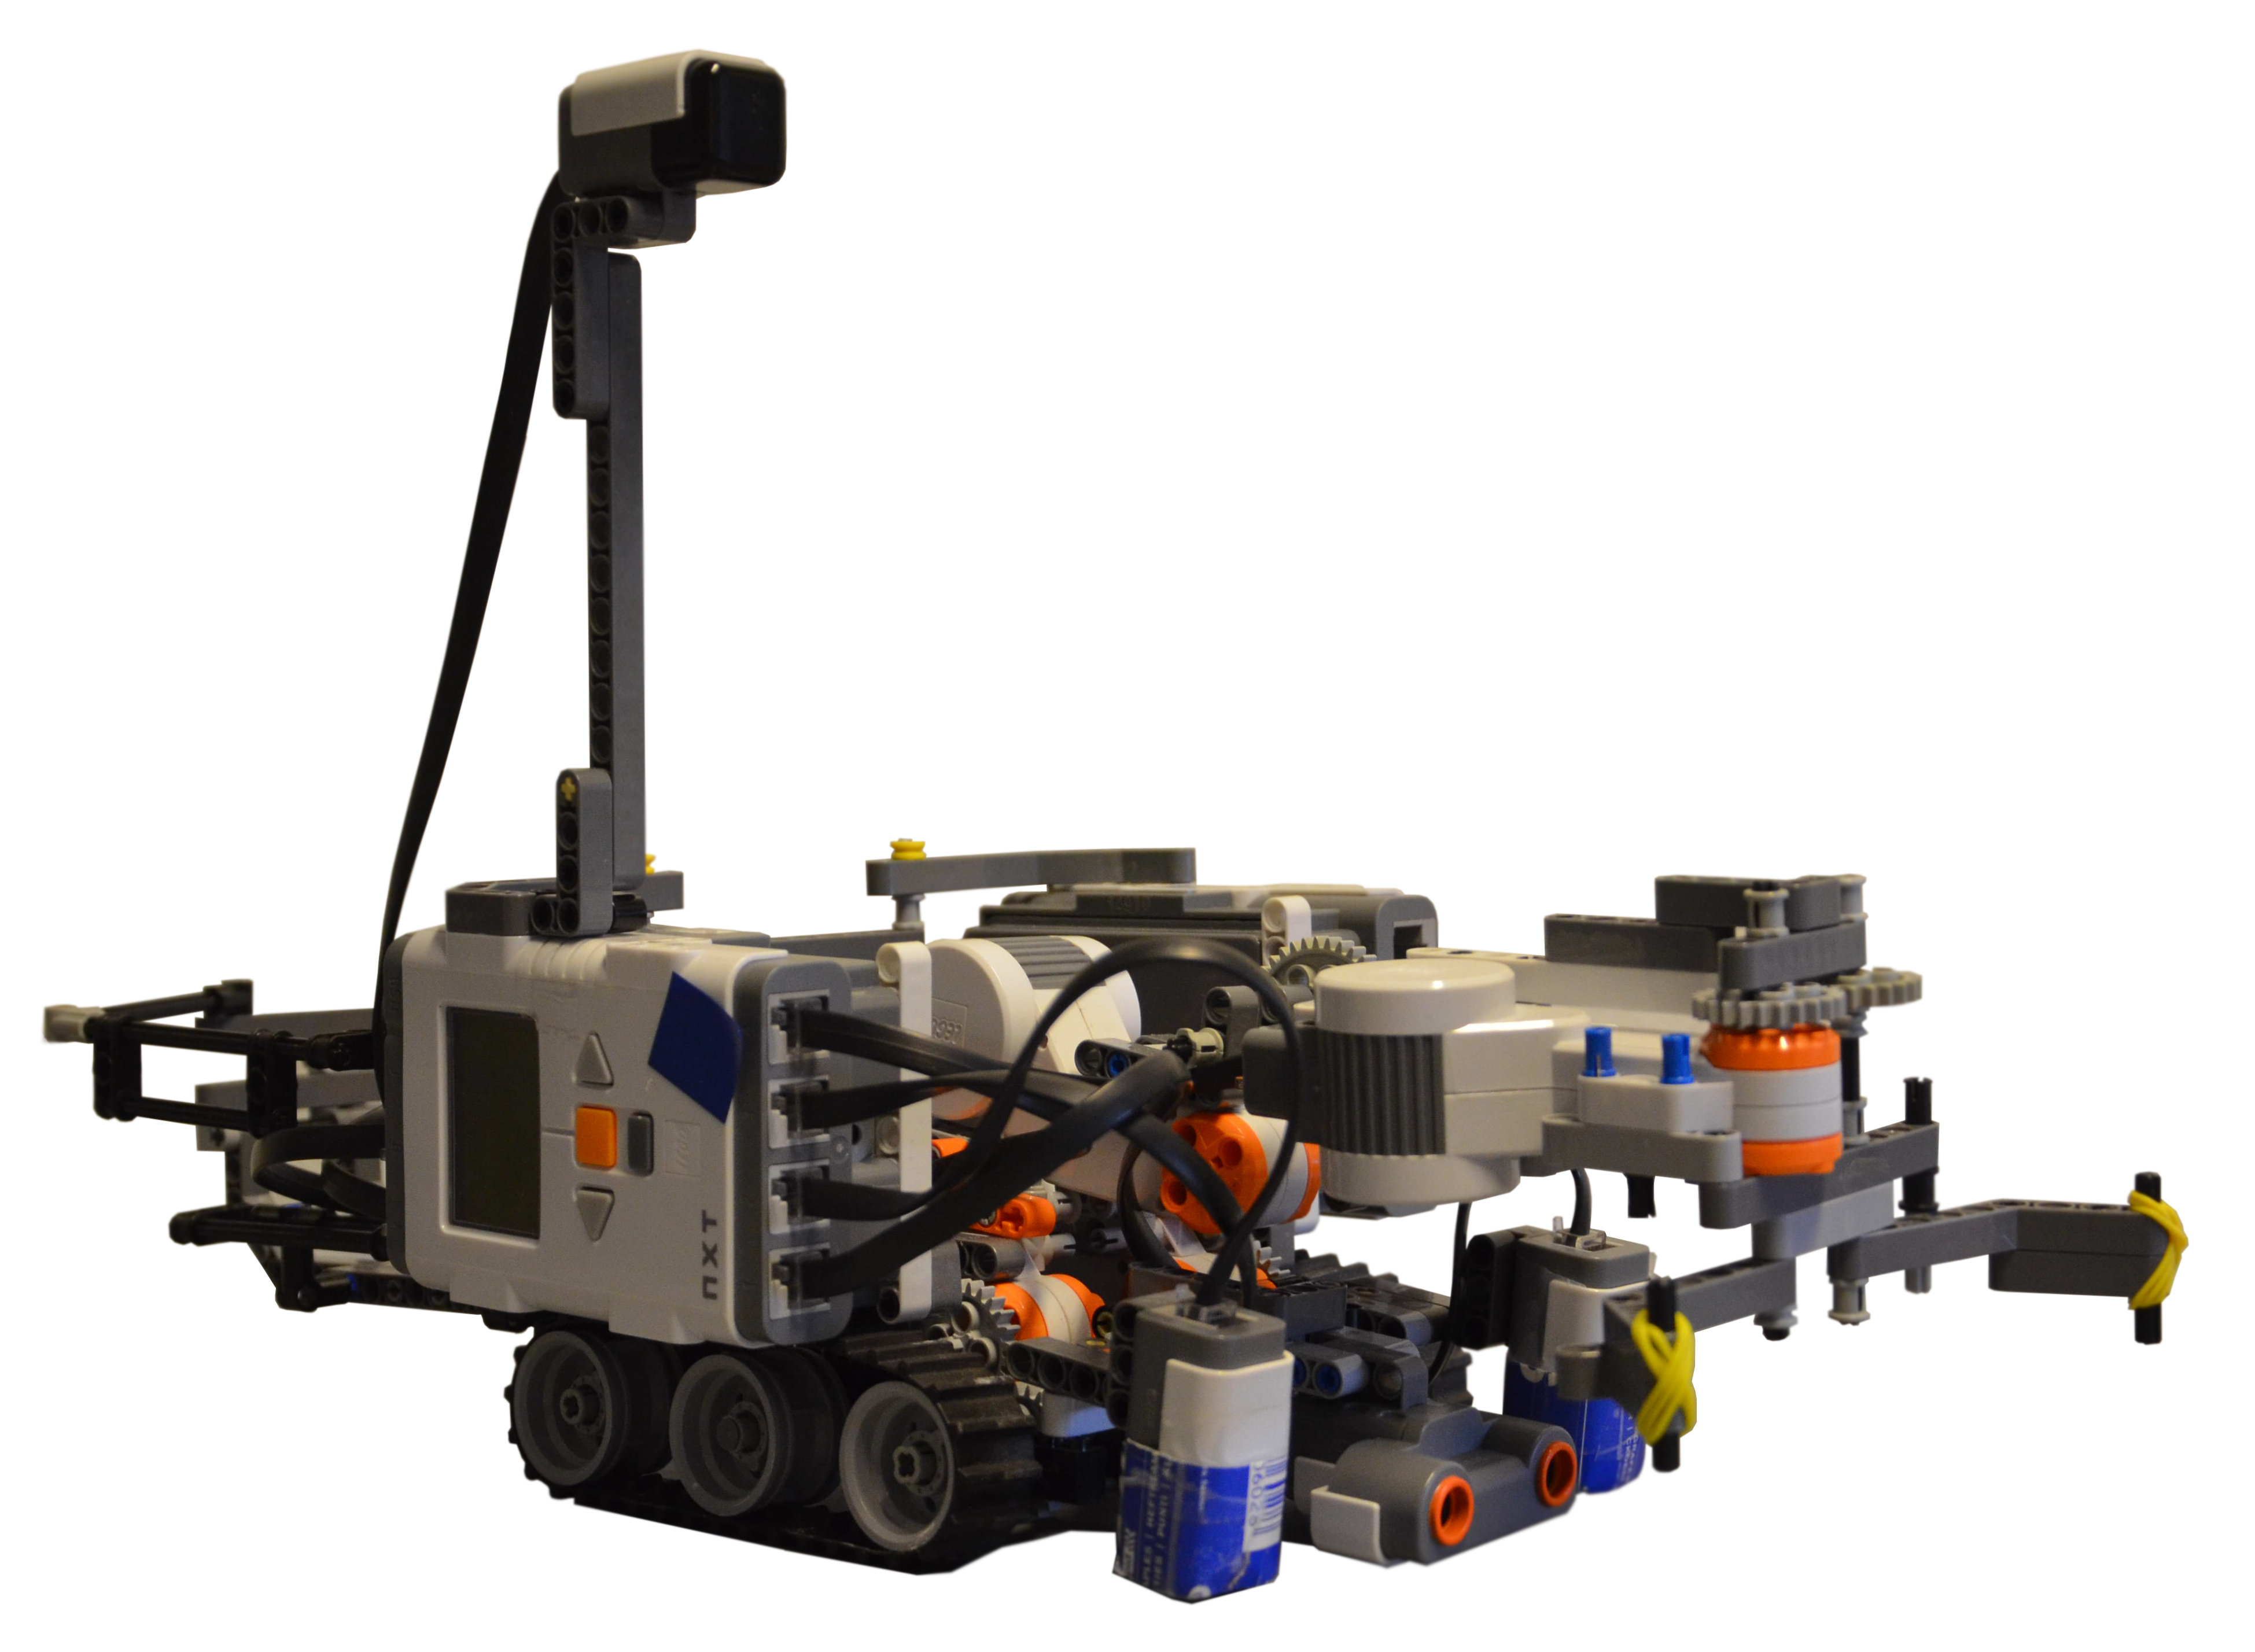
\includegraphics[width=\textwidth]
     {graphics/RobotPhoto2.png}}
\end{figure}

\vspace{2cm} 
\textsc{\Large Software P5 Project \\
Group SW507E14 \\
Aalborg University\\
Fall 2014\\}
\end{flushright}
\cleardoublepage							
\phantomsection
\pdfbookmark[0]{Titlepage}{titlepage}
\thispagestyle{empty}


\begin{minipage}[t]{0.48\textwidth}
\vspace*{-25pt}

\includegraphics[height=4cm]{graphics/AAU-logo-stud-UK-RGB} 
\end{minipage}
\hfill
\begin{minipage}[t]{0.48\textwidth}
{\small 
\textbf{Department of Computer Science}\\
Aalborg University  \\
Software \\
Selma Lagerl\"{o}fs Vej 300 \\
9220 Aalborg Øst} \\
\url{www.cs.aau.dk}
\end{minipage}

\vspace*{1cm}

\begin{minipage}[t]{0.48\textwidth}
\textbf{Title:} \\[5pt]\bigskip\hspace{2ex}
Autonomous Robot Collector\\
\textbf{Theme:} \\[5pt]\bigskip\hspace{2ex}
\parbox{6.6 cm}{
Embedded systems}

\textbf{Project:} \\[5pt]\bigskip\hspace{2ex}
5th semester

\textbf{Project period:} \\[5pt]\bigskip\hspace{2ex}
September 2014 - December 2014

\textbf{Project group:} \\[5pt]\bigskip\hspace{2ex}
SW507E14

\textbf{Participants:} \\[5pt]\hspace*{2ex}
Jacob Elefsen \\\hspace*{2ex}
Patrick Grønhøj \\\hspace*{2ex}
Joakim Iversen \\\hspace*{2ex}
Emil Nesgaard \\\hspace*{2ex}
Mathias Alexander Ibsen \\\hspace*{2ex}
Tobias Hvass Mølbak \\\bigskip\hspace{2ex}

\textbf{Supervisor:} \\[5pt]\hspace*{2ex}
Xike Xie
\vspace*{1cm}

\textbf{Editions: } \\
\textbf{Report pages: \pageref{LastPage}} \\
\textbf{Appendix pages: } \\
\textbf{Completed: }

\end{minipage}
\hfill
\begin{minipage}[t]{0.48\textwidth}
Abstract: \\[5pt]
\fbox{\parbox{7cm}{\bigskipEmbedded systems are everywhere and make up a large percentage of all electronic systems in the world. An embedded system could for example be a robot. For solving small tasks, autonomous robots have become more and more common and have a number of applications in today's society.
\\\\
This project is focused on developing the \projname{}, a prototype robot which can search a limited environment for small objects while collecting these. This idea is the basis for the project. The \projname{} is a prototype, for which the concept could later be expanded into a full scale product.
\\\\
It has been concluded that the \projname{} fulfils the given requirements and works well as a proof of concept. The desired algorithm could not be fully implemented because of sensor inaccuracy so a simpler algorithm with similar efficiency was implemented instead.
\bigskip}}
\end{minipage}

\vfill

{\footnotesize\itshape The content of the report is freely available, but publication (with source reference) may only take place in agreement with the authors.}


\cleardoublepage
\chapter*{Preface}
This report is developed by project group SW507E14 from the department of Computer Science at Aalborg University as part of the fifth semester project from September 2014 to December 2014. The theme of the project is \emph{Embedded Systems} and the focus of this report is developing an autonomous robot.

During the project period, the study method \emph{Problem-based learning}, also known as \emph{The AAU model}, has been used. This report is developed throughout a semester structured like this. This means that the project is heavily focused around using material from the courses. Methods and techniques learned during the courses will be applied throughout the project. It is expected that the reader of this report has knowledge about these methods and techniques.

%This report is written by a group of 5th semester software students at Aalborg University. Throughout the report appropriate terminology is used, which means that the readers must have some knowledge about computer science, more specifically about machine intelligence.

The report uses Harvard citation, that provides the name of the author(s) of the source. As an example, the book used in the course \emph{Machine Intelligence}, is shown as~\citep{artificialintelligencebook}.

~

~

\noindent\begin{tabular}{ll}
%\includegraphics[width=2.5in]
%{Pictures/jacobelefsen.pdf} &  \\
\makebox[2.5in]{\hrulefill} & \makebox[2.5in]{\hrulefill}\\
Jacob Elefsen & Patrick Grønhøj\\[8ex]% adds space between the two sets of signatures
\makebox[2.5in]{\hrulefill} & \makebox[2.5in]{\hrulefill}\\
Mathias Alexander Ibsen & Joakim Iversen\\[8ex]
\makebox[2.5in]{\hrulefill} & \makebox[2.5in]{\hrulefill}\\
Emil Nesgaard & Tobias Hvass Mølbak
\end{tabular}
\cleardoublepage

%%%% Indholdsfortegnelse (TOC) %%%%
\phantomsection
\pdfbookmark[0]{Table of Contents}{contents}
\tableofcontents*

\mainmatter

%%%% Chapters %%%%
% Dette dokument skal ikke indeholde nogen form for tekst!
% Det er en samling af alle kapitlerne.

% Introduction
\chapter{Introduction} \label{cha:introduction}

% Motivation
\section{Motivation} \label{sec:motivation}

As the years go by, new and improved technologies are created and introduced into the world. This progress leads to a number of new ideas that can be implemented. One of these ideas is to automate different monotonous tasks and for this, small robots have been developed. The iRobot Roomba vacuum cleaner~\citep{roomba}, is a robot already well known for being able to perform the, for a human, menial task of vacuum cleaning the house. Similar robots can be found, that can perform similar tasks, such as mowing the lawn or moving goods in a warehouse. Another concept of a robotic helper could be an \textbf{A}utonomous \textbf{R}obot \textbf{C}ollector (\projname{}), a robot which can move around in a limited environment, while collecting small objects in an efficient way. This idea is the basis for this project.

The \projname{}-system stems from a concept, that can be applied to solve a number of menial tasks. As mentioned before, the Roomba can vacuum the floor, but is unable to remove any items which do not belong on the floor, for example toys in a child's bedroom. The \projname{}-system could, potentially, be able to remove items from the floor in a room so that it can be vacuumed, or perhaps collect trash on the sidewalks and roads. The \projname{} could even be combined with the vacuum cleaner - by removing big objects in the path, allowing for the spot to be vacuum cleaned. It could also be used to distribute parcels in an office or warehouse. Another applicable area could be after an event, such as a concert, where the \projname{} has to remove trash to prepare for a new event. A robot which can perform such tasks, while being efficient within a reasonable time, can provide improvements in a number of industries and environments, and with that in mind, the \projname{} has been developed in this project as a proof of concept. The \projname{}-prototype works inside a specified environment, and collect the objects which suit its collection assignment. 

The \projname{} is an intelligent embedded system, with focus on machine intelligence. The common characteristic of an intelligent system is the robot's reasoning, based on an adequate representation of the world with enough information to allow algorithmic solution procedures to be defined. The \projname{} should be able to make intelligent decisions based on the currently perceived state of the environment.

Embedded systems make up a large percentage of all electronic systems in the world(approximately 90\%~\citep{embedded_software_number}). Embedded software can be anything from refrigerators to small wrist watches to intelligent software in modern cars. When developing embedded software some boundaries exist, as the small computers have a limited amount of computational power. These limitations have been taken into account in the design and development of the \projname{} system. 



%Embedded systems make up a large percentage of all electronic systems in the world(approximately 90\%~\citep{embedded_software_number}). Embedded software can be anything from refrigerators to small wrist watches to intelligent software in modern cars. When developing embedded software some boundaries exist, as the small computers have a limited amount of computational power. This must be considered when developing software, as some tasks may require more time to compute than others, which in turn may result in some tasks never being computed. This is especially important in real-time systems, as some tasks may be very important, to ensure that the system functions properly. These limitations have been taken into account in the design and development of the \projname{} system. 


% Physical Requirement
\section{Physical requirements} \label{sec:physical_requirements}
This sections describes the physical requirements that the \projname{} should be able to accomplish. The system's requirements are reflections of the real-life requirements that would allow a similar system to function properly. 

\subsection{Driving}
In order to move around the environment, the robot must be able to drive itself forward and backwards. This is an obvious requirement, however there are numerous non-obvious challenges associated to this. The wheels used must be able to support the frame of the robot while keeping it stable, as well as being able to move straight at an equal speed on a number of surfaces with different friction.

\subsection{Braking}
A requirement of \projname{} is that it should be able to stay within a specified environment. To complete this goal, the robot must be able to brake, to keep itself from overstepping the boundary. Furthermore, as the \projname{} encounters an object, it should be able to stop itself within the correct distance to be able to collect it.

\subsection{Turning}
If the robot is to explore the entirety of the environment, it must be able to turn. It should also be able to turn with at least some precision, since this allows the robot to make reasonable assumptions about its position relative to the environment. 

\subsection{Collecting unit and storage}
The robot must be able to collect objects within a given environment. When a collectible object is encountered, the robot must stop to collect it. The collecting unit picks up the object and the robot stores it within itself and continue to search for more objects to collect. This presents some challenges for the construction of the collecting unit and the robots storage capacity.

The collection unit must be strong enough to pick up objects and place these in the robots storage. The collectible objects can be of varying sizes, which the collection unit must also support. It is required that the collection unit must be able to support picking up objects with a weight of maximum 150-200g and dimensions of 6x6x6cm for square objects and a diameter of 6-7cm for cylinder objects.\fxnote{hvor har vi de tal og vægte fra?}

Another requirement is for the robot to have some place to store the collected objects. The storage is located on the robot itself. The storage capacity of the robot must be sufficiently large to contain multiple objects of the given dimensions. The robot must furthermore be solid enough to support the extra weight of the collected objects. 

%In this project, this environment consists of a flat plane, with the boundaries marked.
%It should also be able to somehow get itself back inside the environment, should it accidentally leave it.
%If it cannot turn precisely, calculating positions in the environment gets hard.
%such that the collecting unit places the picked up objects within this storage, and the robot drives around the environment with the collected objects. 
%Also, if an object is detected in a position in which the robot cannot immediately collect it, it should be able to manoeuvre itself closer and collect it.


% Problem statement
\section{Problem statement} \label{sec:problem_statement}
Based on the motivation from \secref{sec:motivation}, this project focuses on the following problem:

\begin{center}
\textit{How is it possible to develop an autonomous robot which can locate all objects in an environment and collect these objects from the ground, within limited time?}
\end{center}

\subsection{Delimitation} \label{sec:delimitation}
The robot developed in this project is a prototype of the concept mentioned in \secref{sec:motivation}. It is not a final version of the product, that can fulfil the ambition to automate the aforementioned tasks, but a prototype. It is a platform that can be expanded upon in the future. This means, that in order make the implementation of the \projname{}-prototype feasible, certain constraints have been defined. This results in a controlled environment with controlled parameters, where it is more suitable to develop and test a prototype.

\begin{itemize}
\item The environment is a flat plane outlined by black lines that form a convex set of no more than 2 square meters.
\item The robot can only operate with a specified size and shape of objects.
\item The robot does not recognise or otherwise discriminate between objects.
\end{itemize}

%This project concern itself with developing an autonomous robot collector. Given a number of objects to find, the robot should be able to navigate an environment. It should be able to explore all of the environment, looking for objects, until it has found all of these. When it finds an object, it should be able to pick it up utilising a collection unit, and dump the objects in a storage.


% System definition
\section{System definition} \label{sec:system_definition}
This section presents the system definition of the developed project. Collecting small objects in an environment can be a tiresome task, and this robot can automatically pick up objects. The system definition for the \projname{} is the following:

\begin{table}[H]
	\centering
	\begin{narrow}{1cm}{1cm}

	\rule{\linewidth}{0.035cm}
	\begin{center}
	\textbf{System Definition} 
	\end{center}
	\rule{\linewidth}{0.035cm}
    
	\medskip\noindent \textit{Given a number of objects to find, the robot should be able to navigate an environment, defined by black lines, while searching for these objects. While doing this, the robot picks up objects it detects and stores them within its storage container.\fxnote{Opdater denne når projektet har taget sin endelige form}}

	\rule{\linewidth}{0.035cm}
    \label{sec:systemdefinition}
	\end{narrow}
\end{table}




















%As the years go by, new and improved technologies are created and introduced into the world. This progress leads to a number of new ideas, that can be implemented into the world. One of these ideas, is the idea to have self-driving cars, that are able to drive around safely and without interaction from the users. Autonomous cars have already been developed and are being used on the roads. As an example Google has made a working self-driving car~\citep{GoogleCar}. If cars can be made, the possibilities to create a wide range of usable vehicles like ambulances, public transportation, delivery cars and trucks can be developed as well. 

%Autonomous cars can improve the traffic in a number of different ways, if it was an ideal software, that was implemented on all vehicles. First of all, all accidents and crashes could be avoided, if there was some system that made sure that every car followed the rules. This would make the traffic run smoother, and make it more efficient overall. 

%On the smaller scale, robot are being used in private houses and in the industrial sector. Robots can be used 

%This project concern itself with developing an autonomous robot collector. Given a number of objects, the robot should be able to navigate an environment, marked with black tape, by locating the edges and decide that it should not move outside of these. It should be able to explore all of the environment, looking for objects, until it has found all of these. When it finds an object, it should be able to pick it up utilising a crane-claw, and dump the objects in a storage container on the back of the robots frame.

% Analysis
\chapter{Analysis} \label{cha:analysis}

This chapter contains the needed analysis before the \projname{} can be designed. The chapter gives a description on how to model the problem as well as the platform chosen to implement the \projname{} on. Furthermore, the tests of the different sensors and motors, as well as the results of the tests will be described.

% Problem description
\section{Problem description} \label{sec:problem-description}

The problem that the \projname{}-prototype has to solve, is to collect a number of objects within a given environment. It has to do this by driving to and collecting every object, after they have been located. The issue of locating the objects is complex, and the question of how the robot can ensure that all objects in the environment has been found, is hard to answer. To do this, one would have to be able to confirm, whether or not all possible locations have been checked.

Once all objects have been found, the problem is to find a path between all the objects, that the robot can then follow in order to pick them up. This path is known as a hamiltonian path; it must visit all locations exactly once. The problem, however, is not finding a path, since many such paths exist -- rather, the problem is to find an acceptable route that preferably is as close to the optimal path as possible.

The optimal path between the objects would be the path that is most efficient. Multiple variables affect the efficiency, for instance power used, computations required or distance travelled. However in this project, the focus will be to reduce the time spent from start to completion. In a real scenario, you would want the \projname{} to be reasonably fast at cleaning up an area, or at completing any other given task, so it makes sense to use it instead of doing the task yourself.

To achieve a faster completion time, reducing distance travelled to a reasonable level compared to the shortest possible path, will be the focus of this report. This problem is known as the \emph{travelling salesman problem}, and is NP-hard \citep{tsp}. To find the shortest route, one would have to calculate the distance of every possible route between the objects, which has a calculation complexity of $\mathcal{O}(n!)$. This is obviously not feasible, and thus heuristics will be used in following chapters to develop algorithms that can solve the problem within an acceptable time limit.




% Model
\section{Modelling the problem} \label{sec:model}

When constructing autonomous robots like the \projname{}, a few techniques exist to model the robot's known world. It is also important to know what exactly makes an autonomous robot, autonomous. In order for a robot to be autonomous it should be able to make decisions based on the current state the robot is in, previous experiences, and according to the goals that need to be accomplished~\citep{artificialintelligencebook}. 

\begin{figure}[H]
     \center{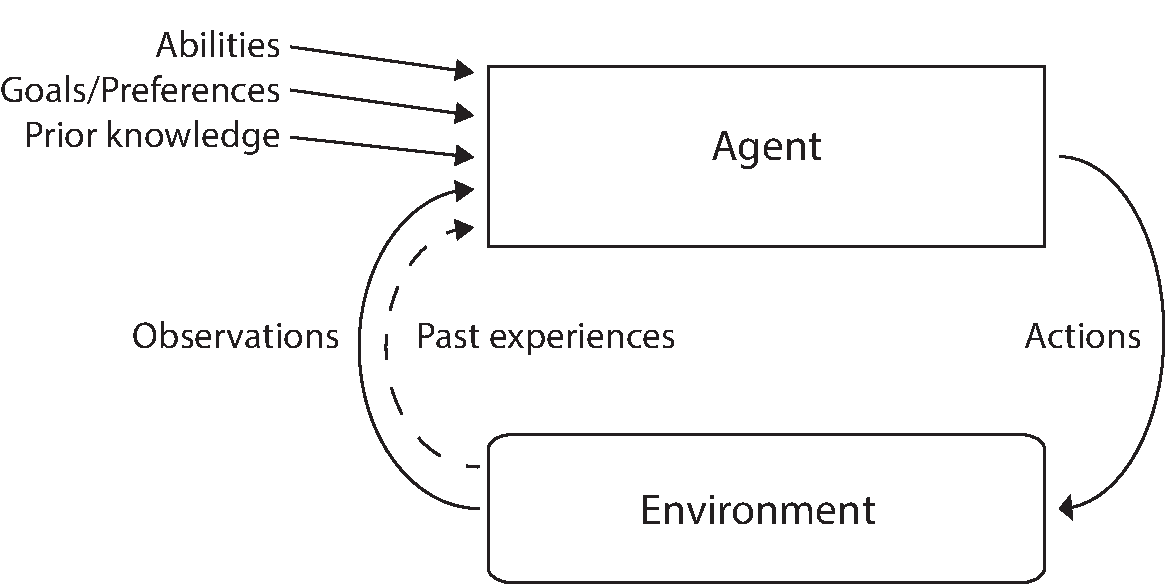
\includegraphics[width=320pt]
     {graphics/AgentModel.pdf}}
     \caption{\label{fig:model_mi_agent} An agent in an environment.}
\end{figure}

\figref{fig:model_mi_agent} shows an agent, something that acts in an environment, what prior knowledge this agent has and what actions the agent can do to interact with the environment. The \projname{} has the following capabilities:

\begin{description}
\item[Abilities] Abilities are the actions the agent can use to interact with the world. The \projname{} is able to move around the environment by driving forward, backwards and turning. It can sense objects and detect the environment boundaries. It is also able to pickup objects and place these into the attached storage container.  
\item[Goals/Preferences] Goals are the objectives that the agent must complete. The \projname{} should be able to collect all the objects inside the environment within reasonable time. Preferences are rules for which action the robot performs, if two different actions are available and neither necessarily moves it closer to the goal. For instance, which way the robot should turn when it encounters a boundary.
\item[Prior knowledge] The robot will not have any knowledge about the environment beforehand. Other than the programmed logic, it will only know how many objects to collect before halting.
\item[Observations] Knowledge about the current environment. This is obtained by sensors and knowledge of how far the \projname{} has driven. 
\item[Past experiences] Knowledge about how many objects has been collected. 
\end{description}

Despite sounding similar, there is a slight difference between prior knowledge and past experience. The difference is that prior knowledge is information that has been hard coded into the robot, while past experience is something it has learnt by itself. The only past experience \projname{} is collecting is how many objects it has found so far. If it had kept knowledge about previous runs and used it to try and find the new objects faster, it would have been machine learning, which is not a part of this project.

In order for the robot to understand the world, it must contain a suitable representation. There are three different ways to represent a world - \emph{State-based}, \emph{Feature-based} and \emph{Relational}~\citep{artificialintelligencebook}. Each of these are shortly discussed and the most suitable is used to model the problem. 

\begin{description}
\item[State-based] In a state-based representation, each state represents a possible model of the world. If the entire environment, i.e. knowledge about the boundary, location of the robot, and object position, should be described using a state-based representation, then a  tremendous amounts of states would be needed to provide the necessary information. The world should also be big enough to precisely place the objects and contain the space in between these. 

%A slightly altered version of the state-based representation would be to have a state for each phase of the \projname{}'s behaviour. These states could, for instance, be a \emph{Searching for objects} or \emph{Collecting objects} states. This would greatly decrease the amount of states needed, and still make a state-based representation possible. \fxnote{ibsen: jeg tror ikke det her holder. du repræsenterer jo ikke som sådan env., bare robotten}

\item[Feature-based] In a feature-based representation, every state can be described in terms of features, where a feature has a value in each state. The entire environment can be represented with a two-dimensional array, in the feature based representation. Each point describes a spot in the environment, where either an object is located, boundary is spotted, or if nothing is in that spot. 

Another way to use the feature-based representation, would be to describe the environment, as known by the robot, according to the values provided by the sensors. This way, the \projname{} could reason on the provided values, to determine, for instance, if the colour sensor values matches the values for the boundary. These could also determine if an object has been seen, if the object is inside some specified object distance. 

\item[Relational] A relational representation deals with relational descriptions in terms of individuals and relations among them. This can be used to describe states of individuals or their position compared to others. 
\end{description}

The feature-based representation of the world, would suit the project well. Though, the feature-based representation, where the entire environment would have to be mapped, would require a lot of memory to initialise and update the representation continuously. This would also require that the sensors are accurate enough to find the correct position of the objects. The simpler feature-based representation would be a possible way to represent the world for the \projname{}. 


%Both a state-based and a feature-based representation of the world suits the project. The feature-based representation, where the entire environment would have to be mapped, would require a lot of memory to initialise and update the representation continuously. This would also require that the sensors are accurate enough to find the correct position of the objects. The simple state-based model, by using phases, would be a possible solution for the \projname{} as well.  \fxnote{ibsen: det her skal rettes igennem for teoretiske fejl via MI slides... tror ikke det holder}



% Platform
\section{Platform} \label{sec:platform}
To build the \projname{}, a platform has to be chosen. There exist multiple platforms for which it is possible to develop an autonomous robot such as the \projname{}. This section looks into some of the most accessible platforms to consider when creating an embedded system. The chosen platform is further described along with its specifications.

\subsection{Arduino}
The first platform considered was the Arduino. The Arduino single-board micro controller is an open-source hardware platform, intended to make the creation of small, interactable devices accessible to students. As such, it has a fairly low price. The Arduino comes with a fully equipped Integrated Development Environment (IDE), and can be programmed in either C or C++~\citep{arduino}.

\subsection{Raspberry Pi}
Another platform that was considered for the \projname{} was the Raspberry Pi. The Raspberry Pi is developed by the Raspberry Pi Foundation as a single board computer, the size of a credit card. It is a microcomputer, which is able to perform various tasks, such as word processing and video transmitting. The specifications vary depending on the model. Model A, has a 700MHz CPU, 256MB memory and needs a SD card for storage. The operating system(OS) is based on Linux and two of the available OSes are Raspbian and Arch Linux~\citep{raspberry_pi}. 

\subsection{Lego NXT} \label{sec:lego_nxt}
The last considered platform was the LEGO Mindstorm NXT 2.0. It consists of a series of sensors and actuators that are all connected to a programmable NXT Intelligent Brick(NXT brick). The construction itself can be built with bricks from the LEGO Technic series. The primary component in the Mindstorm NXT series is the NXT brick, which is used to control the components connected the it. The NXT brick has four input sockets which can be used for various sensors and three output sockets which are used to send signals to the motors that controls the robot~\citep{lego_nxt_2.0}.

\subsection{Choice of platform}
All of these three platforms are good choices for creating an embedded system. Each of them have their positive and negative aspects, but in regards to the requirements of the \projname{} it was been decided that the Lego NXT is the most suitable platform for this project.

LEGO NXT includes motors and sensors built for the NXT. All sensors and motors as well as the NXT brick itself are constructed in such a way, that they are straightforward to assemble with the LEGO Technic parts. 

Furthermore, LEGO NXT has been widely used for building robotic projects in the faculty and it was therefore the natural choice. The actual construction of the body of the robot is more cumbersome with the Arduino or Raspberry Pi. Getting the electronics working requires a lot of wiring and soldering while building the actual body might require welding the parts together and generally put a lot more emphasis on the physical components. New device drivers would also have to be written for the sensors and motors to function. This would require effort and time, outside the scope of the project, and by choosing the LEGO NXT this extra time can be used to program the \projname{}.





% Hardware
\section{Hardware choices and limitations}\label{sec:hardware}

This section describes the choices made for the project in terms of which hardware is required to construct the \projname{} prototype. In order for the robot to solve the tasks described in \secref{sec:system_definition}, some specific hardware is required. The hardware required for the robot is:

\begin{itemize}
\item Two motors to drive and steer the robot.
\item Two motors for collecting objects.
\item Two sensors to ensure that the robot stays inside the boundaries of the environment.
\item One sensor to detect objects.
\item One sensor for movement precision.
\end{itemize}

There exist a number of available sensors and actuators for the LEGO NXT. These sensors gives the NXT robots the ability to perform various actions. For the required tasks, it has been chosen to use the interactive servo motors for driving, steering, and the collection of objects. The colour sensor is well suited to ensure that the robot can detect the environment boundaries. For detecting objects, the ultrasonic sensor has been chosen, as the robot is required to know when an object is present and should be collected, as well as the distance to the detected object. Finally, to help ensure precise movement, the HiTechnic NXT Compass sensor is used.

Because the NXT brick only has output sockets for three motors, and the \projname{} will use at least four, two NXT bricks are required. This will require communication between the bricks, which is possible due to the NXT brick's integrated Bluetooth, which allows interaction between the multiple NXT bricks in a master-slave relationship with a maximum of 3 slaves pr. master. This allows the master-brick to send commands to the slave-bricks' output sockets and because of that, a single brick is able control more than the three motors a single NXT brick otherwise would be limited to~\citep{lego_edu_guide}.

\subsection{Hardware test} \label{sec:hardware_test}
In order to know the capabilities and limitations of the hardware, some tests were conducted. Testing environments were set up to test the individual hardware devices. The early tests were created in LabView and transferred to the NXT brick. These used the original LEGO NXT firmware. During the test the LEGO brick would write all the results into a file, which later would be transferred into LabView for analysis. 

Further tests were conducted using the data logging feature. A Bluetooth connection is established between the NXT brick and a PC, and while the robot is running, the outputs from the sensors and motors are logged and sent to the PC. The data can be saved in a .csv file and converted into graphs, which makes for easy analysis.

\subsubsection{Ultrasonic sensor} \label{sec:ultrasonic_sensor}
The ultrasonic sensor emits an ultrasonic sound wave and measures the time it takes for the wave to impact on an object and return to the sensor. Depending on the time taken, the sensor can measure the distance from the sensor to the detected object~\citep{lego_education}. 

\begin{figure}[H]
     \center{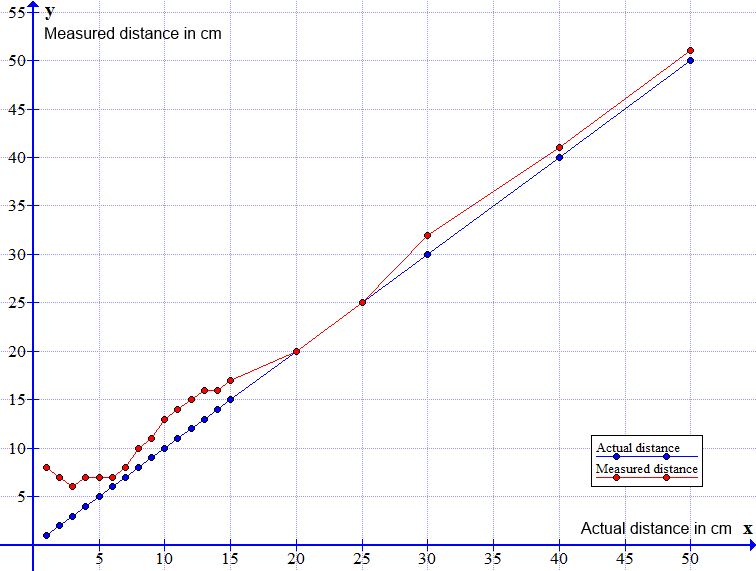
\includegraphics[width=320pt]
     {graphics/DistanceGraph.png}}
     \caption{\label{fig:ultrasonic_sensor_test_graph} The actual distance and the measured distance from the ultrasonic sensor test.}
\end{figure}

The ultrasonic sensor was tested at different distances to measure the accuracy. The test was performed stationary and every 25 ms it sends out a pulse, for 250 seconds, resulting in 1000 pulses, which would give a significant average of the distance. \appref{app:ultrasonic_sensor_test} shows the raw values observed during the test, which has been converted into the graph seen in \figref{fig:ultrasonic_sensor_test_graph}. The graph shows values from the tests from 1 cm to 50 cm. This test was performed using LabView.

\begin{figure}[H]
     \center{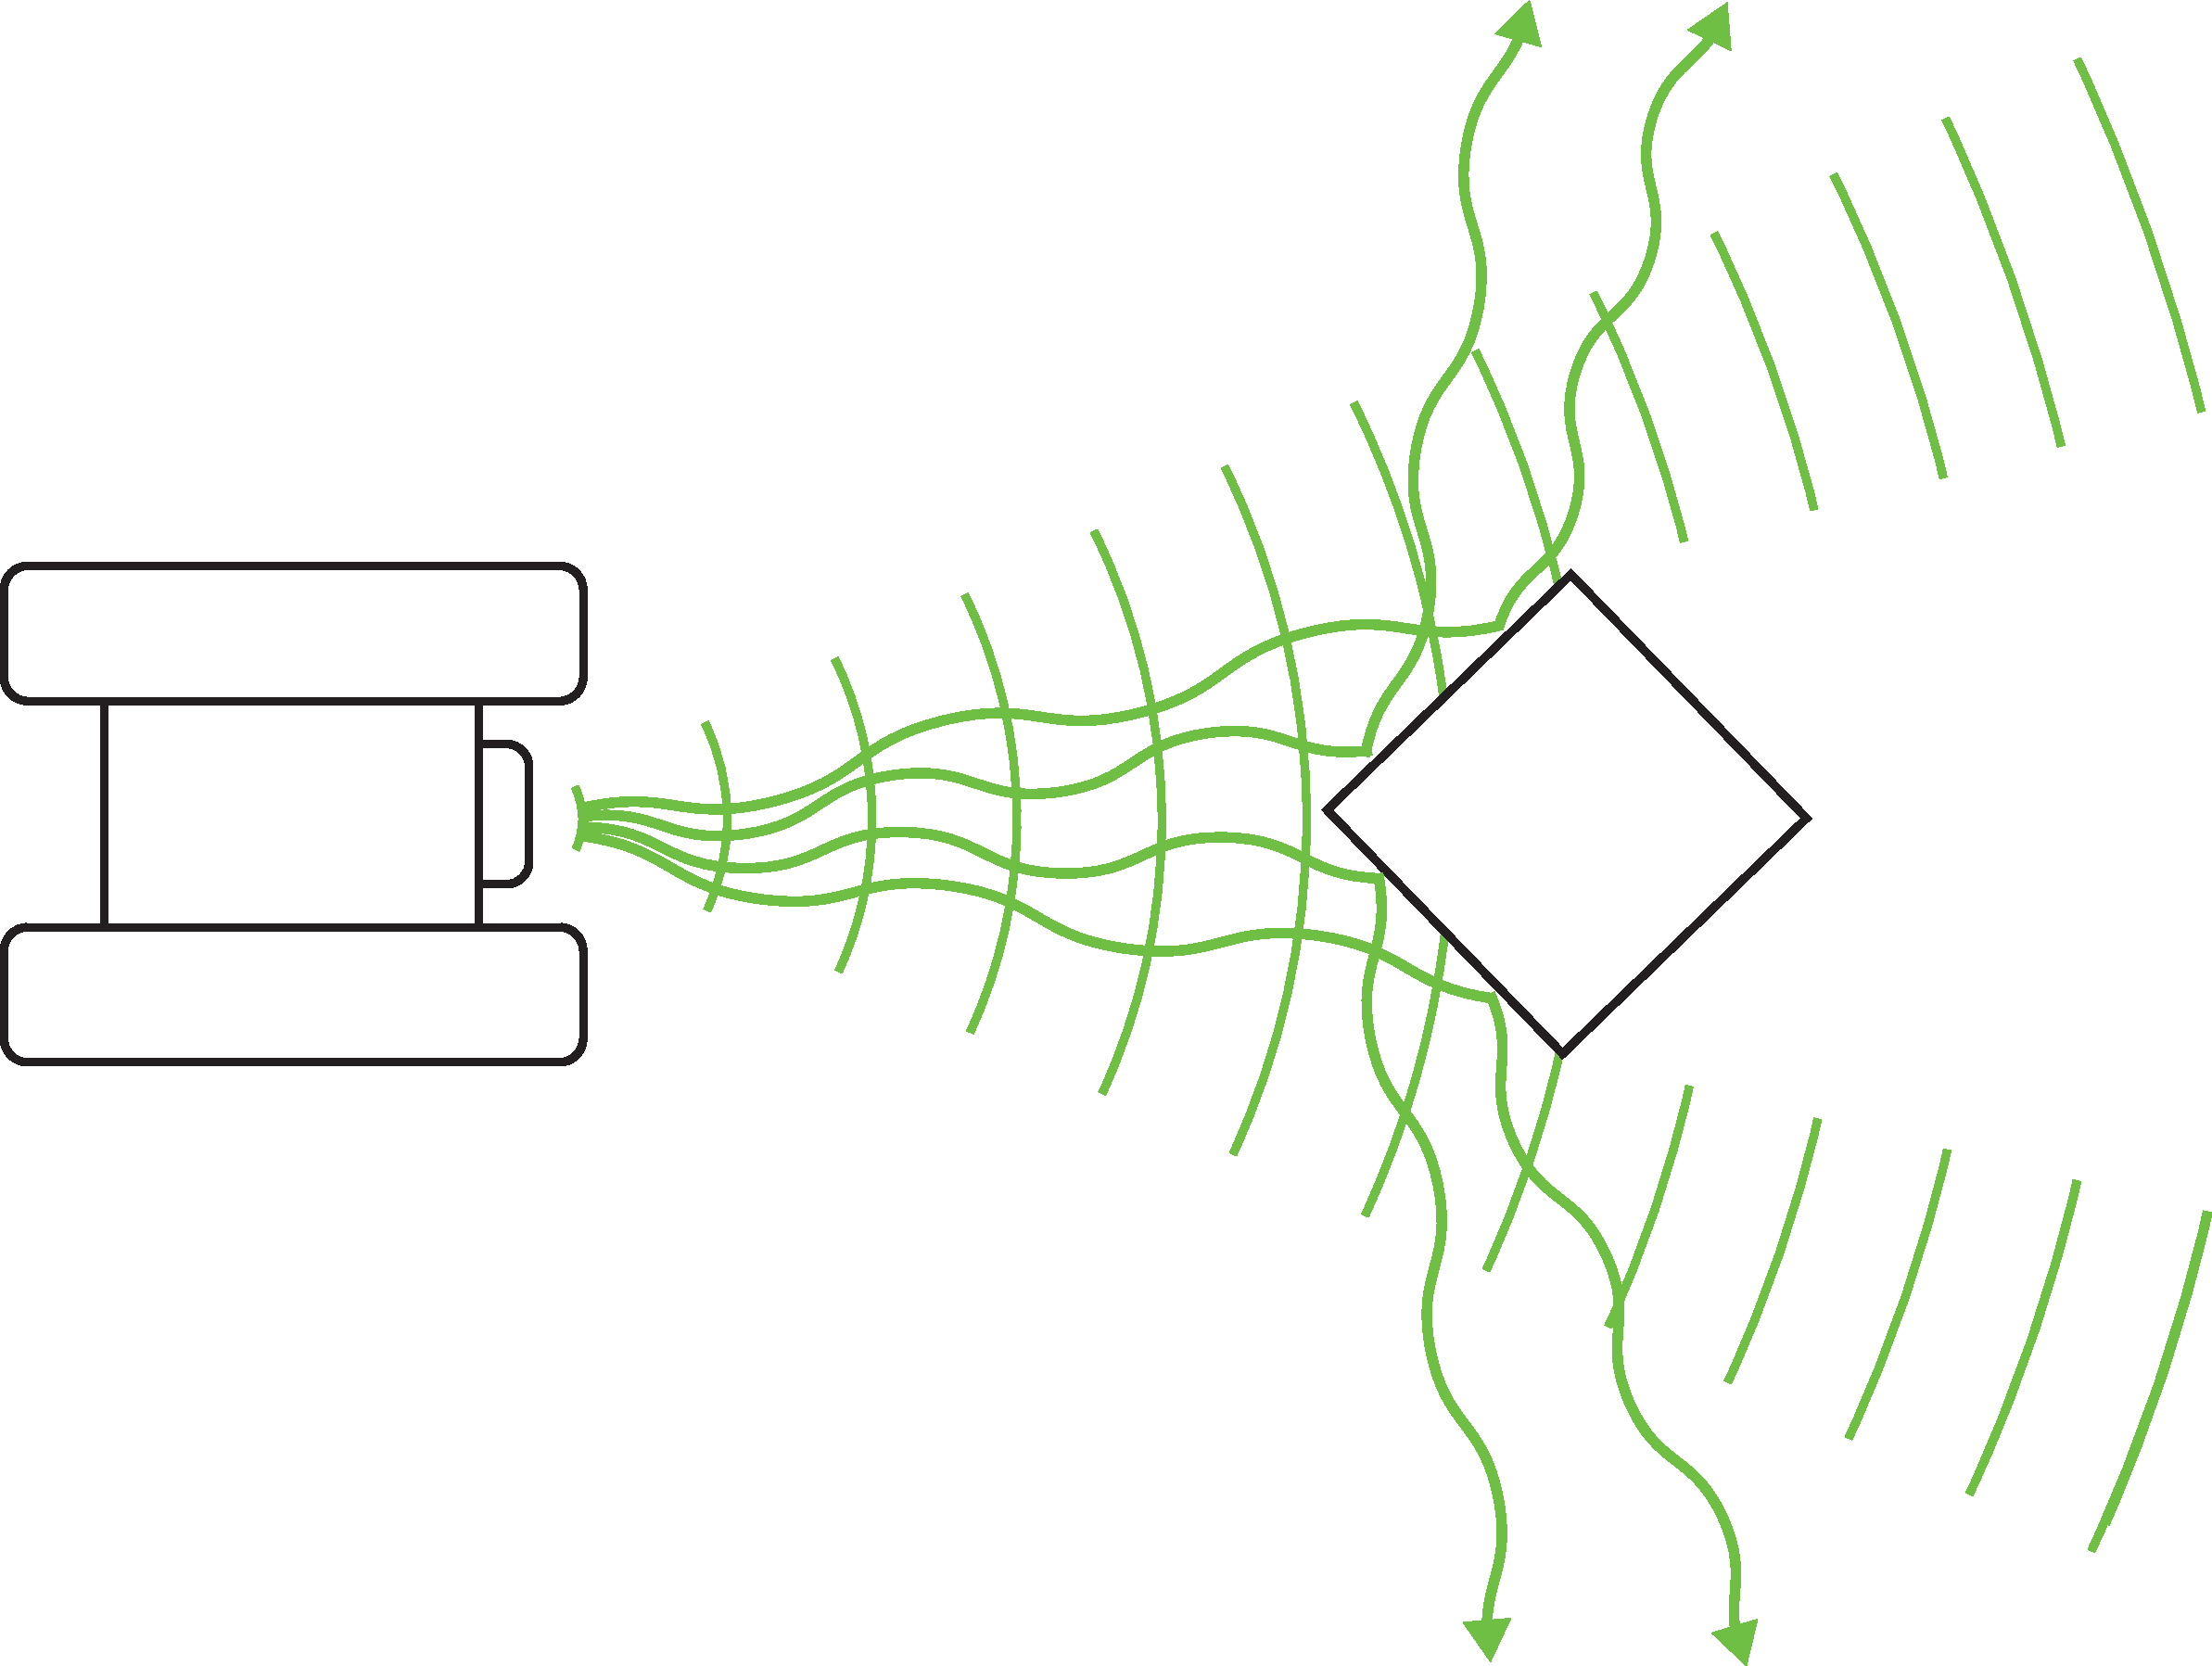
\includegraphics[width=320pt]
     {graphics/SonarWaves.pdf}}
     \caption{\label{fig:angled_object} Sonic waves on an angled object.}
\end{figure}

At short distances, the ultrasonic sensor is proved to be imprecise. This is most highly due to the quality of the sensor and how it is constructed. As seen in \figref{fig:ultrasonic_sensor_test_graph}, the values vary a few cm. The sensor have some problems when it comes to spotting an object at certain angles, for example the angled object illustrated in \figref{fig:angled_object}. The sound waves sent out is reflected away from the sensor. This results in the sensor not being able to correctly calculate the distance and sometimes not being able see the object at all.

\begin{figure}[H]
     \center{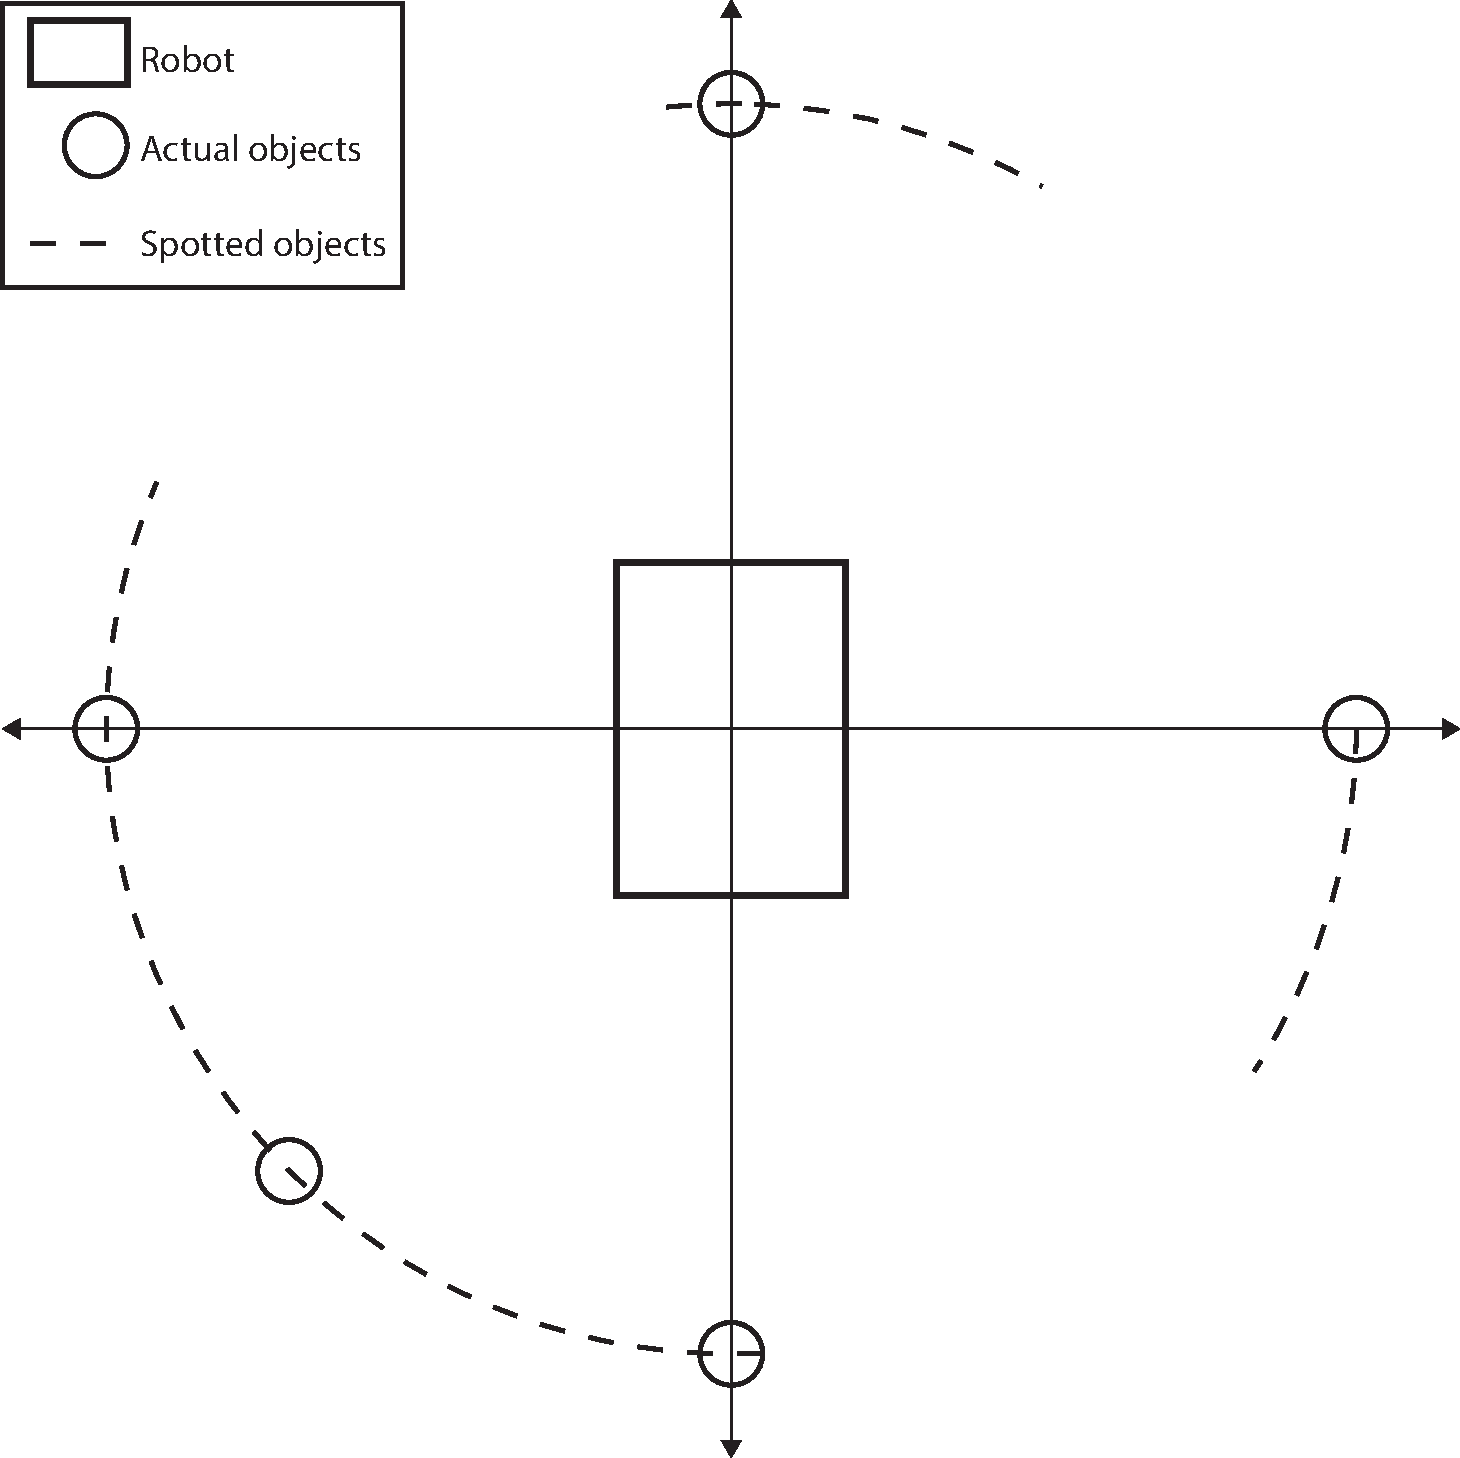
\includegraphics[width=320pt]
     {graphics/SonarTest.pdf}}
     \caption{\label{fig:sonar-test-drawing} 360 degree test with ultrasonic sensor. Graph can be seen in \appref{app:sonar-test-graph}.}
\end{figure}

Last but not least the ultrasonic sensor is having trouble spotting multiple objects if they are standing too close, as seen on the last three objects on \figref{fig:sonar-test-drawing}. It is a matter of the cone being too wide and the first object not being out of sight before the next one is spotted. This results in only one object being added to the object array which means that the \projname{} will get into trouble once it starts collecting.\\
Sometimes the robot is encountering the opposite problem, because sometimes the sound waves does not return despite targeting an object. This break in incoming waves will result in the robot thinking that this is a new object and it will therefore add the same object again.

\subsubsection{Colour sensor} \label{sec:colour_sensor} 
The colour sensor can, by sending out light, measure the reflected light that returns to the sensor. The sensor now contains some raw RGB values, which it can provide the users, or use the integrated colour detecting mechanism to decide which colour it has observed~\citep{lego_education}. 

The test was performed to test the colour sensors ability to detect the black colour which is used as the environment boundary. The sensor should be placed close to the ground, as the only task is to detect the boundary. It should be possible to see a clear difference between the black boundary and the floor. The minimum and maximum values of the black boundary needs to be detected so that \projname{} can distinguish between the floor and the black boundary. Each sensor is tested, where the test provided their respective min and max values after 500 tries. In the end the absolute smallest and largest value is used for each RBG value. This was performed on the boundary and the floor to see the difference between these. A test was also performed, when passing over the black boundary to get the respective values and compare these to the min and max values from the previous test.

\begin{figure}[H]
     \center{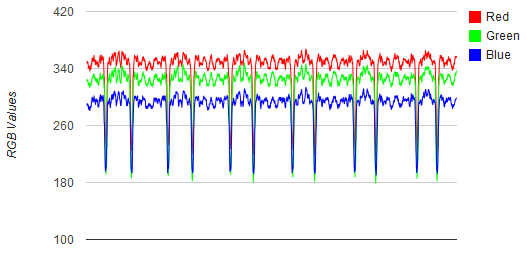
\includegraphics[width=\textwidth]
     {graphics/ColorLeft.png}}
     \caption{\label{fig:colour_sensor_test_left} Graph showing RGB values passing the black boundary 12 times for the left colour sensor.}
\end{figure}

\begin{figure}[H]
     \center{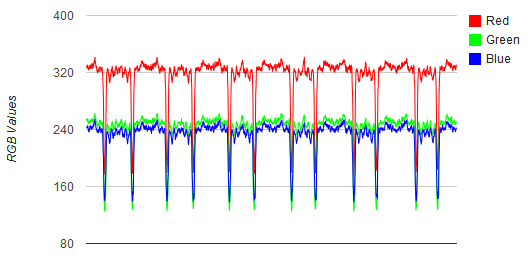
\includegraphics[width=\textwidth]
     {graphics/ColorRight.png}}
     \caption{\label{fig:colour_sensor_test_right} Graph showing RGB values passing the black boundary 12 times for the right colour sensor.}
\end{figure}

As seen on \figref{fig:colour_sensor_test_left} and \figref{fig:colour_sensor_test_right}, the two sensors are quite different when it comes to the values they provide, despite being tested the exact same way. This is important and must be taken into account when using the sensors in the program. Due to uncertainties from the environment such as light, shadows, or dust, even the values in the two figures aren't always accurate. To counter this, it is possible to increase the range between the black minimum and maximum detection values to reduce potential detection problems. This increased range is possible, because the floor RGB values compared with the black values are quite different, allowing the addition of this \emph{extended range}.

\begin{table}[H]
	\centering
	\ra{1.3}
	\rowcolors{3}{Gray}{}
    \begin{tabular}{|l|r|r|r|r|r|r|r|r|}
    \hline
    \rowcolor{DGray}
    \textbf{Sensor} & \multicolumn{4}{c|}{Right} & \multicolumn{4}{c|}{Left} \\ \hline
    \rowcolor{Gray}
    \textbf{Surface} & \multicolumn{2}{c|}{Black boundary} & \multicolumn{2}{c|}{Floor} & \multicolumn{2}{c|}{Black boundary} & \multicolumn{2}{c|}{Floor}   \\ \hline
    \rowcolor{DGray}
    \textbf{Colour range}  & Min~~~~ & Max~~~ & Min~~~ & Max~~~ & Min~~~~ & Max~~~ & Min~~~ & Max~~~ \\ \hline
\multicolumn{1}{|l|}{Red}  & 187     & 260    & 329    & 334    & 209     & 282    & 349    & 354    \\ \hline
\multicolumn{1}{|l|}{Green}& 127     & 192    & 252    & 256    & 173     & 253    & 327    & 332    \\ \hline
\multicolumn{1}{|l|}{Blue} & 147     & 198    & 242    & 248    & 182     & 240    & 292    & 297    \\
    \hline
    \end{tabular}
    \caption{\label{table:colour_sensor_test} Colour sensor results on the black boundary and the floor.}
\end{table}

In~\tblref{table:colour_sensor_test}, the min and max values for each sensor is listed. The values reflect the data on \figref{fig:colour_sensor_test_left} and \figref{fig:colour_sensor_test_right}. These values provide the base line for the RGB value range.


\subsubsection{Compass sensor}
The HiTechnic NXT Compass Sensor is a digital compass that measures the earth's magnetic field and returns a value representing the current heading in degrees. The magnetic heading is returned as an integer from 0 to 359, where 0 is north and 180 is south~\citep{compass}.

The test of the compass sensor is performed the following way: First the sensor is calibrated to work optimally with the \projname{}. The NXT bricks and the motors on the robot have their own magnetic fields which are noise to the compass sensors readings. This makes sensor calibration prior to use a necessity for accurate output values. The compass sensor will furthermore be placed at least 15cm from the motors and 10cm from the NXT bricks~\citep{compass}.

After the initial calibration the robot is placed facing in a direction close to north, which means a heading of around 0 degrees. The robot then performs a 720 degrees spin while the heading is being logged. Turning clockwise the returned value should be a linear increasing value from 0 and up, until 0 degrees is hit again when the robot is facing north. Turning counter-clockwise, the returned value should quickly jump to 359 degrees and linearly decrease while spinning, until north is found again. This will repeat for every 360 degrees the robot does.

\begin{figure}[H]
     \center{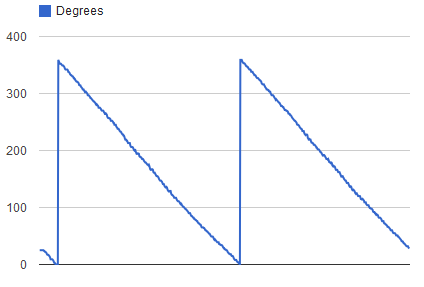
\includegraphics[width=320pt]
     {graphics/DegreesGraph.png}}
     \caption{\label{fig:compass_sensor_test_graph} The measured degrees from a 720 degrees counter clockwise turn.}
\end{figure}

\figref{fig:compass_sensor_test_graph} shows the result of a test, where the robot is turning counter-clockwise. The graph illustrates that the compass sensor is outputting the expected values, and thus works as intended. 

\subsubsection{Interactive servo motor} \label{sec:servo_motor}
The LEGO NXT interactive servo motor enables movement. The motors have built-in reduction gear assemblies with internal rotation sensors that measures speed and distance and reports it back to the NXT brick. This allows for a more precise motor control and the ability to run the motor in steps with one degree of accuracy~\citep{lego_education}.

As the \projname{} has to be able to move around and pick up objects, it would be suitable to drive in a straight line if need be. Therefore the servo motors have been tested to get an idea of a possible difference in performance. The test was set to run for 10 seconds on each motor and measure the how many steps they each managed to run. It was also conducted at different power levels, as the accuracy could vary, depending on the speed. 

\begin{table}[H]
	\centering
	\ra{1.3}
	\rowcolors{1}{Gray}{}
    \begin{tabular}{lccc}
    \hline  
    \rowcolor{DGray}
    \textbf{Power Level}~~~~~~~~~~~~ & Motor L(Steps) & Motor R(Steps) & Difference \\ \hline 
    100\%                  & 6,658                  & 6,666                & 0,12\% \\
    90\%                   & 5,823                  & 5,912                & 1,51\% \\
    80\%                   & 5,192                  & 5,262                & 1,33\% \\
    70\%                   & 4,495                  & 4,571                & 1,67\% \\
    60\%                   & 3,859                  & 3,923                & 1,64\% \\
    50\%                   & 3,145                  & 3,211                & 2,07\% \\
    40\%                   & 2,479                  & 2,551                & 2,86\% \\
    \hline 
    \end{tabular}
    \caption{\label{table:servo_motor_test} Servo motor test of rotations.}
\end{table}

As \tblref{table:servo_motor_test} shows, at higher power levels the difference is the smallest, compared to the lower power level, where the difference is increased. This will have an impact on the movement and precision of the \projname{}, which must be taken into account and adjusted when developing. The construction of the \projname{} has put some restrictions on the minimal speed. The minimal power level value is around 40\%. Tests have shown that using power levels beneath this value can make the motors fail. Despite the motors driving similar at maximum speed is it not an acceptable speed level. The ultrasonic sensor is not able to register objects when rotating at this speed.

\subsubsection{Object specification} \label{sec:object_specification}
Since the \projname{} is considered a prototype, there are restrictions on the objects it is able to collect. The size of the robot, the strength of the motors and the positions of the objects, all presents some limitations on what objects that can be collected by the \projname{}. The different considerations regarding the objects' attributes are:

\begin{itemize}
\item Size - Can the claw get a hold on the object - and detect it? 
\item Weight - Can the motors lift the object? 
\item Shape - Can it hold the object and not let go?
\item Angle - Can the ultrasonic sensor detect the object from all angles?
\end{itemize}

It is possible to detect objects of 1 cm in width, if the object is placed exactly in the middle of the ultrasonic sensor. If the object is over 12 cm in width, the claw is unable to collect the object. Given the position of the claw compared to that of the ultrasonic sensor, square objects of size 6x6x6 cm, or cylinder objects with a diameter of 6-7 cm are preferred.

Different weight of objects have been tested for the robots strength. The robot's limit is around 150-200 g depending on the object's surface friction. It does not matter if the object weight is close to 0 g, although the robot tend to push around the objects while trying to grab and if the object is too light, there is a risk that it might tip over.

The shape of the object is important; if for instance an object is placed in a way where the ultrasonic sensor's sound waves are not immediately reflected back to the sensor, incorrect values will be provided. Square objects with a sharp corner, are hard to detect and constitute a serious problem to the \projname{}. This is described in \secref{sec:ultrasonic_sensor}. 

If an object is a cylinder, the surface of the object is round, meaning the sound waves are always reflected the same way, no matter how it's angled. This means that it will either always be hard, or always be easy, finding cylindrical objects, since the angle is irrelevant. This has been tested with different kinds of cans and the robot was always able to detect the cans and always returned proper values. It is not enough for the final version to only work with cylindrical-shaped objects, but for the prototype version of the \projname{}, it is a reasonable restriction.





% Design
\chapter{Design} \label{cha:design}

With the prior analysis done, some design decisions for the robot can be made. This chapter will contain a description of all the design decisions the implementation of the \projname{} will be based on. A platform has already been chosen, but there is also the matter of choosing the optimal operating system. The chosen operating system and the reasons for why it was chosen will be explained. Afterwards the the functionality of the robot will be described, as well as the chosen algorithm for solving the problem. This will result in some final requirements for the \projname{}-

%With the platform specified and the necessary hardware tested, the time has come to choose which firmware to install on the LEGO NXT. Along with that comes a description of the libraries used by the language that comes with the chosen firmware. The different sensors, motors, and features of the robot, that were tested in \secref{sec:hardware}, will be further described and explained.

% Language
\section{Operating system and programming language} \label{sec:os_and_proglanguage}
Since the LEGO Mindstorm NXT was chosen as the platform for the prototype robot, it puts some limitations on the choice of OS and programming language. It is required to use an OS that is supported by the NXT Intelligent Brick and the programming language must furthermore be supported by the chosen OS.

A few different OSes were considered for the \projname{}. The default NXT firmware IDE allows for simple drag-and-drop programming in the accompanying LEGO NXT-G software, for creating simple sample robots quickly. Another IDE called BricxCC, also used with the default firmware, uses the programming language Not eXactly C (NXC) and Next Byte Codes (NBC). The default firmware allows for programming both simple and more advanced robots. 

A considered custom firmware was leJOS NXJ, that uses the programming language Java. The leJOS NXJ OS contains a tiny Java virtual machine to execute the code \citep{lejos}. This implies that, had this OS been chosen, the source code would be written in Java.

Another of the considered custom firmwares is nxtOSEK. nxtOSEK is a hybrid between the device drivers of leJOS NXJ, the TOPPERS/ATK Kernel, and the TOPPERS/JSP Real-Time OS. It supports programming in ANSI C/C++ using GCC (GNU ARM) and contains a C and C++ API for the NXT sensors and motors~\citep{nxtosek, toppers_atk, toppers_jsp, nxtOSEK2, nxtosek_api}.

nxtOSEK supports multithreading and real-time multi tasking features, and more importantly for the \projname{}, events are also supported. Bluetooth connection is supported, both brick to brick, and brick to pc, where R/C and Data Logging possibilities exist.

The default OS is more restrictive than some of the alternatives. Because of this, it was decided use one of the custom firmwares. The C/C++ languages were favoured over Java and were the main reason why nxtOSEK was chosen over leJOS.







%Since the LEGO Mindstorm NXT was chosen as the platform for the prototype robot, it puts some limitations on the choice of OS and programming language. It is required to use an OS that is supported by the NXT Intelligent Brick and the programming language must furthermore be supported by the chosen OS.

%A few different OSes were considered for the \projname{}. The default NXT firmware IDE allows for simple drag-and-drop programming in the accompanying LEGO NXT-G software, for creating simple sample robots quickly. Another IDE called BricxCC, also used with the default firmware, uses the programming language Not eXactly C (NXC) and Next Byte Codes (NBC). NXC is a high-level open-source language similar to the C language, build on the NBC compiler. 

%The default firmware and the supported programming languages and tools associated, allows for programming both simple and more advanced robots. However it is still more restrictive than some of the alternatives. Because of this, it was decided to look at a couple of custom firmwares.  

%One of the considered custom firmwares was leJOS NXJ, that uses the programming language Java. The leJOS NXJ OS contains a tiny Java virtual machine to execute the code \citep{lejos}. It also includes all classes in the NXJ API \citep{nxj} as well as all the tools needed to upload programs to the NXT brick. This implies that, had this OS been chosen, the source code of this project would be written in Java and then apply Java methods to invoke the API.

%Another of the considered firmwares is nxtOSEK. nxtOSEK is a hybrid between the device drivers of leJOS NXJ, the TOPPERS/ATK Kernel, and the TOPPERS/JSP Real-Time OS, along with further code to make these work together. It supports programming in ANSI C/C++ using GCC (GNU ARM) and contains a C and C++ API for the NXT sensors and motors. The C and C++ API calls are available through ECRobot, that extends the C++ language with the necessary commands to manipulate the LEGO NXT hardware~\citep{nxtosek, toppers_atk, toppers_jsp, nxtOSEK2, nxtosek_api}.

%nxtOSEK includes a variety of useful features. Like leJOS it contains all the tools needed to upload programs to the NXT brick. It is possible to use the Eclipse CDT IDE to write and compile programs and upload them to the NXT brick. It supports multithreading and real-time multi tasking features provided by TOPPERS, and more importantly for the \projname{}, events are also supported. It supports Bluetooth connections, both from the brick to PC and from NXT Brick to NXT Brick. Furthermore, connecting a brick to the PC through Bluetooth, R/C and Data Logging features is provided by the NXT Gamepad.

%The C/C++ languages were favoured over Java and were the main reason why nxtOSEK was chosen over leJOS.

%BricxCC \citep{bricxcc} is an Integrated Development Environment (IDE) for programming LEGO NXT robots on the default firmware. BricxCC includes support for programming the LEGO Mindstorms NXT brick using the programming languages Not eXactly C (NXC) and Next Byte Codes (NBC). NBC is a simple open-source language with an assembly language syntax, and NXC is a high-level open-source language similar to C, built on the NBC compiler.



%The default firmware and the supported programming languages and tools associated, allows for programming both simple and more advanced robots. However it is still more restrictive than some of the alternatives. Because of this, it was decided to look at a couple of custom firmwares. One of the considered custom firmwares was leJOS. The leJOS NXJ \citep{lejos} OS contains a tiny Java virtual machine to execute the users code. It also includes all classes in the NXJ API \citep{nxj} as well as all the tools needed to upload programs to the NXT brick. It supports programming in an object-oriented language, Java. This implies that, had this OS been chosen, the source code of this project would be written in Java or a similar language that can be compiled to Java bytecode and then apply Java methods to invoke the API.

%The last of the considered OSes, which also was the one chosen for this project, was nxtOSEK. nxtOSEK \citep{nxtosek} is a hybrid between the device drivers of leJOS NXJ, the TOPPERS/ATK \citep{toppers_atk} Kernel, and the TOPPERS/JSP \citep{toppers_jsp} Real-Time OS, along with further code to make these work together. It supports programming in ANSI C/C++ using GCC (GNU ARM) and contains a C and C++ API for the NXT sensors and motors. The C and C++ API calls are available through ECRobot, described in \secref{subsec:ecrobot}. These languages were favoured over Java and were the main reason why nxtOSEK was chosen over leJOS.

%nxtOSEK includes a variety of useful features. Like leJOS it contains all the tools needed to upload programs to the NXT brick. It is possible to use the Eclipse CDT IDE to write and compile programs and upload them to the NXT brick. It supports multithreading and real-time multi tasking features provided by TOPPERS, and more importantly for the \projname{}, events are also supported. It supports Bluetooth connections, both from the brick to PC and from brick to brick (one NXT to another NXT). This means that two NXT bricks can communicate with each other and be used in a master-slave relationship. Furthermore, connecting a brick to the PC through Bluetooth, R/C and Data Logging features is provided by the NXT Gamepad.

%\subsection{ECRobot} \label{subsec:ecrobot}
%Along with the nxtOSEK firmware comes the ECRobot API. This extends the C++ language with the necessary commands to manipulate the LEGO NXT hardware. The ECRobot C API was originally developed for a MATLAB Model-Based Design environment for the first LEGO Mindstorm NXT release. With the release of LEGO NXT 2.0 a ECRobot C++ API was developed. The update from C to C++ took the ECRobot from a structured imperative API to an object oriented API, which allowed the different motors and sensors to be sorted into device classes~\citep{nxtosek_api}.



%control the motors and different input sensors.

% Functionality description
\section{Functionality description} \label{sec:functionality_description}
In this section the overall functions and the different parts of the \projname{} are described. The fully built \projname{} includes four sensors and four servo motors, which means that it also includes two NXT Bricks, as it only supports three outputs pr. Brick for the motors. The robot drives in the environment, using the interactive servo motor until it locates an object, using the ultrasonic sensor, or the black boundary using the colour sensor. If it locates an object, the master brick transmit a signal to the slave brick to commence the arm task. During this time, the robot stands still, waiting on a signal. All the components and how they are connected to the NXT Bricks is shown in \figref{fig:robot_overview}. 

\subsection{Brick communication}
The two LEGO NXT bricks used for the robot is required to communicate in order to start and stop certain tasks. The integrated Bluetooth 2.0 module is used for communication between the NXT Bricks. One of the two LEGO NXT Bricks is chosen to be the master and the other one is the slave. The master unit controls the primary task of the robot, while the slave is used to handle a smaller, parallel task when receiving instructions from the master unit.

\subsection{Colour sensor} 
The robot is equipped with two colour sensors on the front of the robot, at each side. This is used to detect the black lines that specify the boundary of the environment. Based on the returned light the colour sensors return the RGB value to the LEGO NXT brick. The two colour sensors are handled by the master unit. 

\subsection{Ultrasonic sensor}
The ultrasonic sensor is placed in the front of the robot, just under the claw. This is used to detect the distance to the objects in front of the robot. The master unit is controlling the ultrasonic sensor.
%The ultrasonic sensor can measure the distance from the sensor to other objects. The robot use the ultrasonic sensor for detecting the distance to other object in front of the robot. The ultrasonic sensor are also controlled by the master unit. 

\subsection{Compass sensor}
The compass sensor is placed on the top or the robot, at the end of an arm, so that it is located as far from the bricks and motors as possible. This is to reduce the noise from the bricks and motors magnetics fields. The sensor is pointing in the same direction as the robot.

The compass sensor is used to help ensure precision in the robots movement. This increased precision in movement is used when searching for objects, and when turning to the exact degree where the next object is located. When the object are discovered during the scanning phase, their location are mapped according to distance and the angle between them.

\subsection{Interactive servo motor}
The four interactive servo motors is used for two tasks. The first task is to move the robot around the environment. This includes driving forward, backward, and turning. The second task is the arm and the claw. This task consist of squeezing the claw around a detected object and holding this until the arm has reached the point, where the claw can let go of the object, and this lands in the storage behind the robot. Then the arm returns to the starting position, ready to grab a hold of new objects. Both task use 2 motors. The driving task is handled by the master unit, and the arm task is handled by the slave unit.

\subsection{Motor controller}
The tests in \secref{sec:servo_motor} proves that the motors used in the project are not very precise. It was decided to implement a motor controller to solve the precision issues. The objective for the motor controller is to ensure that the motors reach the same distance at the same time. 

The controller takes as input how many steps each motor has turned at any given time. Based on the steps, and the direction, the speed is increased or decreased on the left motor. The left motor is selected as the motor where the speed is changed, and the right motor moves at constant speed. The motor controller also ensures that the robot stops at the targeted number of steps $+/-$ an acceptable error margin.

It is not possible to make the motors 100\% precise because of the minimum speed for driving the robot is too high. This is due to the construction of the robot. To deal with this problem, a reasonable error margin is chosen. The error margin is used in two cases: First if the motors difference in steps is inside this error margin the robots speed is not adjusted. Secondly if the motor is inside the target steps, the robot will stop moving.  

The result of the controller is a robot that, even though the hardware is imprecise, moves straight and behave as expected.


$motorR\_ahead \leftarrow Motor~L~steps~<~Motor~R~steps$
$motorL\_ahead \leftarrow Motor~L~steps~>~Motor~R~steps$



$moving\_forward$

$ motor\_power\_increased \leftarrow moving\_forward \land motorR\_ahead \land \lnot motorL\_ahead$


$motor_power_decreased \leftarrow $ 

\fxnote{Se link i kommentar under fxnote}
% http://artint.info/html/ArtInt_106.html

\begin{figure}[H]
     \center{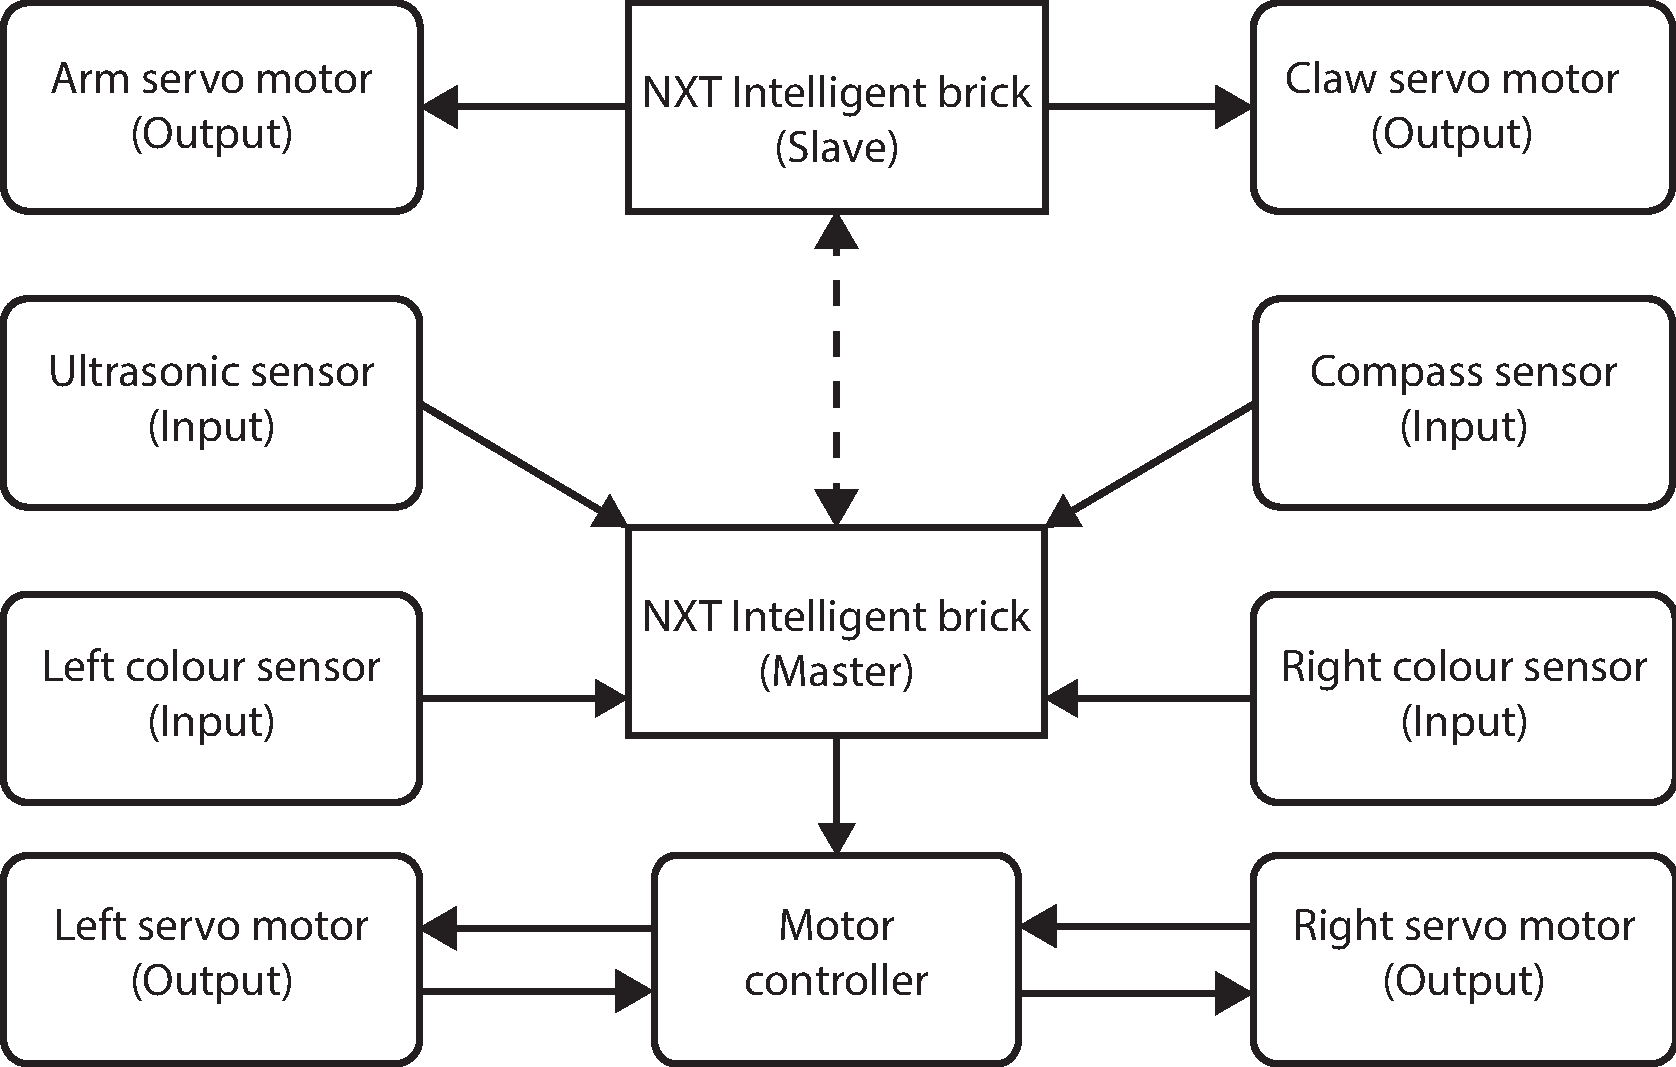
\includegraphics[width=\textwidth]
     {graphics/ComponentDiagram.pdf}}
     \caption{\label{fig:robot_overview} Diagram of all the components included in the robot.}
\end{figure}



% Algorithm design
\section{Algorithm design} \label{sec:algorithm-design}

In order to solve the \emph{travelling salesman problem}, as described in \secref{sec:problem-description}, a heuristic is needed. Since it is not feasible to solve the problem of finding the optimal path, an algorithm that provides an acceptable solution will be chosen instead.

Two algorithms have been proposed and designed in this project: one is more intelligent and takes all the relative distances between the objects into account, while the other is very reactive. These two algorithms are, respectively, the \emph{nearest neighbour (NN) algorithm} and the \emph{next-in-view (NIV) algorithm}.


\subsection{Nearest neighbour algorithm} \label{sec:nn-algorithm}
The NN-algorithm starts by doing a 360 degrees turn while scanning the nearby area around it for objects. The distance and angle for each object are saved and when the robot is done scanning, a route will be calculated using trigonometry and the NN-algorithm concepts. These calculations will result in an array of instructions containing distances and angles. Each instruction will take the robot from the current position to the next object following the calculated route. The robot should scan after completing the route, to ensure that all objects has been collected, in case it didn't collect all of the objects. The \projname{} computes the entire route before moving.

The algorithm uses trigonometry to select the next object, by using the current position, the starting position and the position of the next object. These positions are in relation to the starting position, where all the objects positions were found. The amount of degrees the \projname{} must turn, in order to get to the same heading as the next object, is saved as instructions, along with the distance that needs to be travelled in order to get to it. 

These instructions must then be followed after the route has been calculated. \figref{fig:object_navigation_first} shows a situation where all the objects have been spotted, and now the \projname{} must decide which object that should be collected first. At this point the shortest object is easy to conclude, as the distance to all objects, from the starting position, is already known, based on information from the ultrasonic sensor. The shortest distance overall is found, and saved along with the heading, and the object associated to this is remembered, and marked as collected, to remove this from consideration when finding the next objects. Another set of instructions is used to ensure that the \projname{} is pointing back, at the starting position. This is used to ease the calculations of the following objects. 

\begin{figure}[H]
     \center{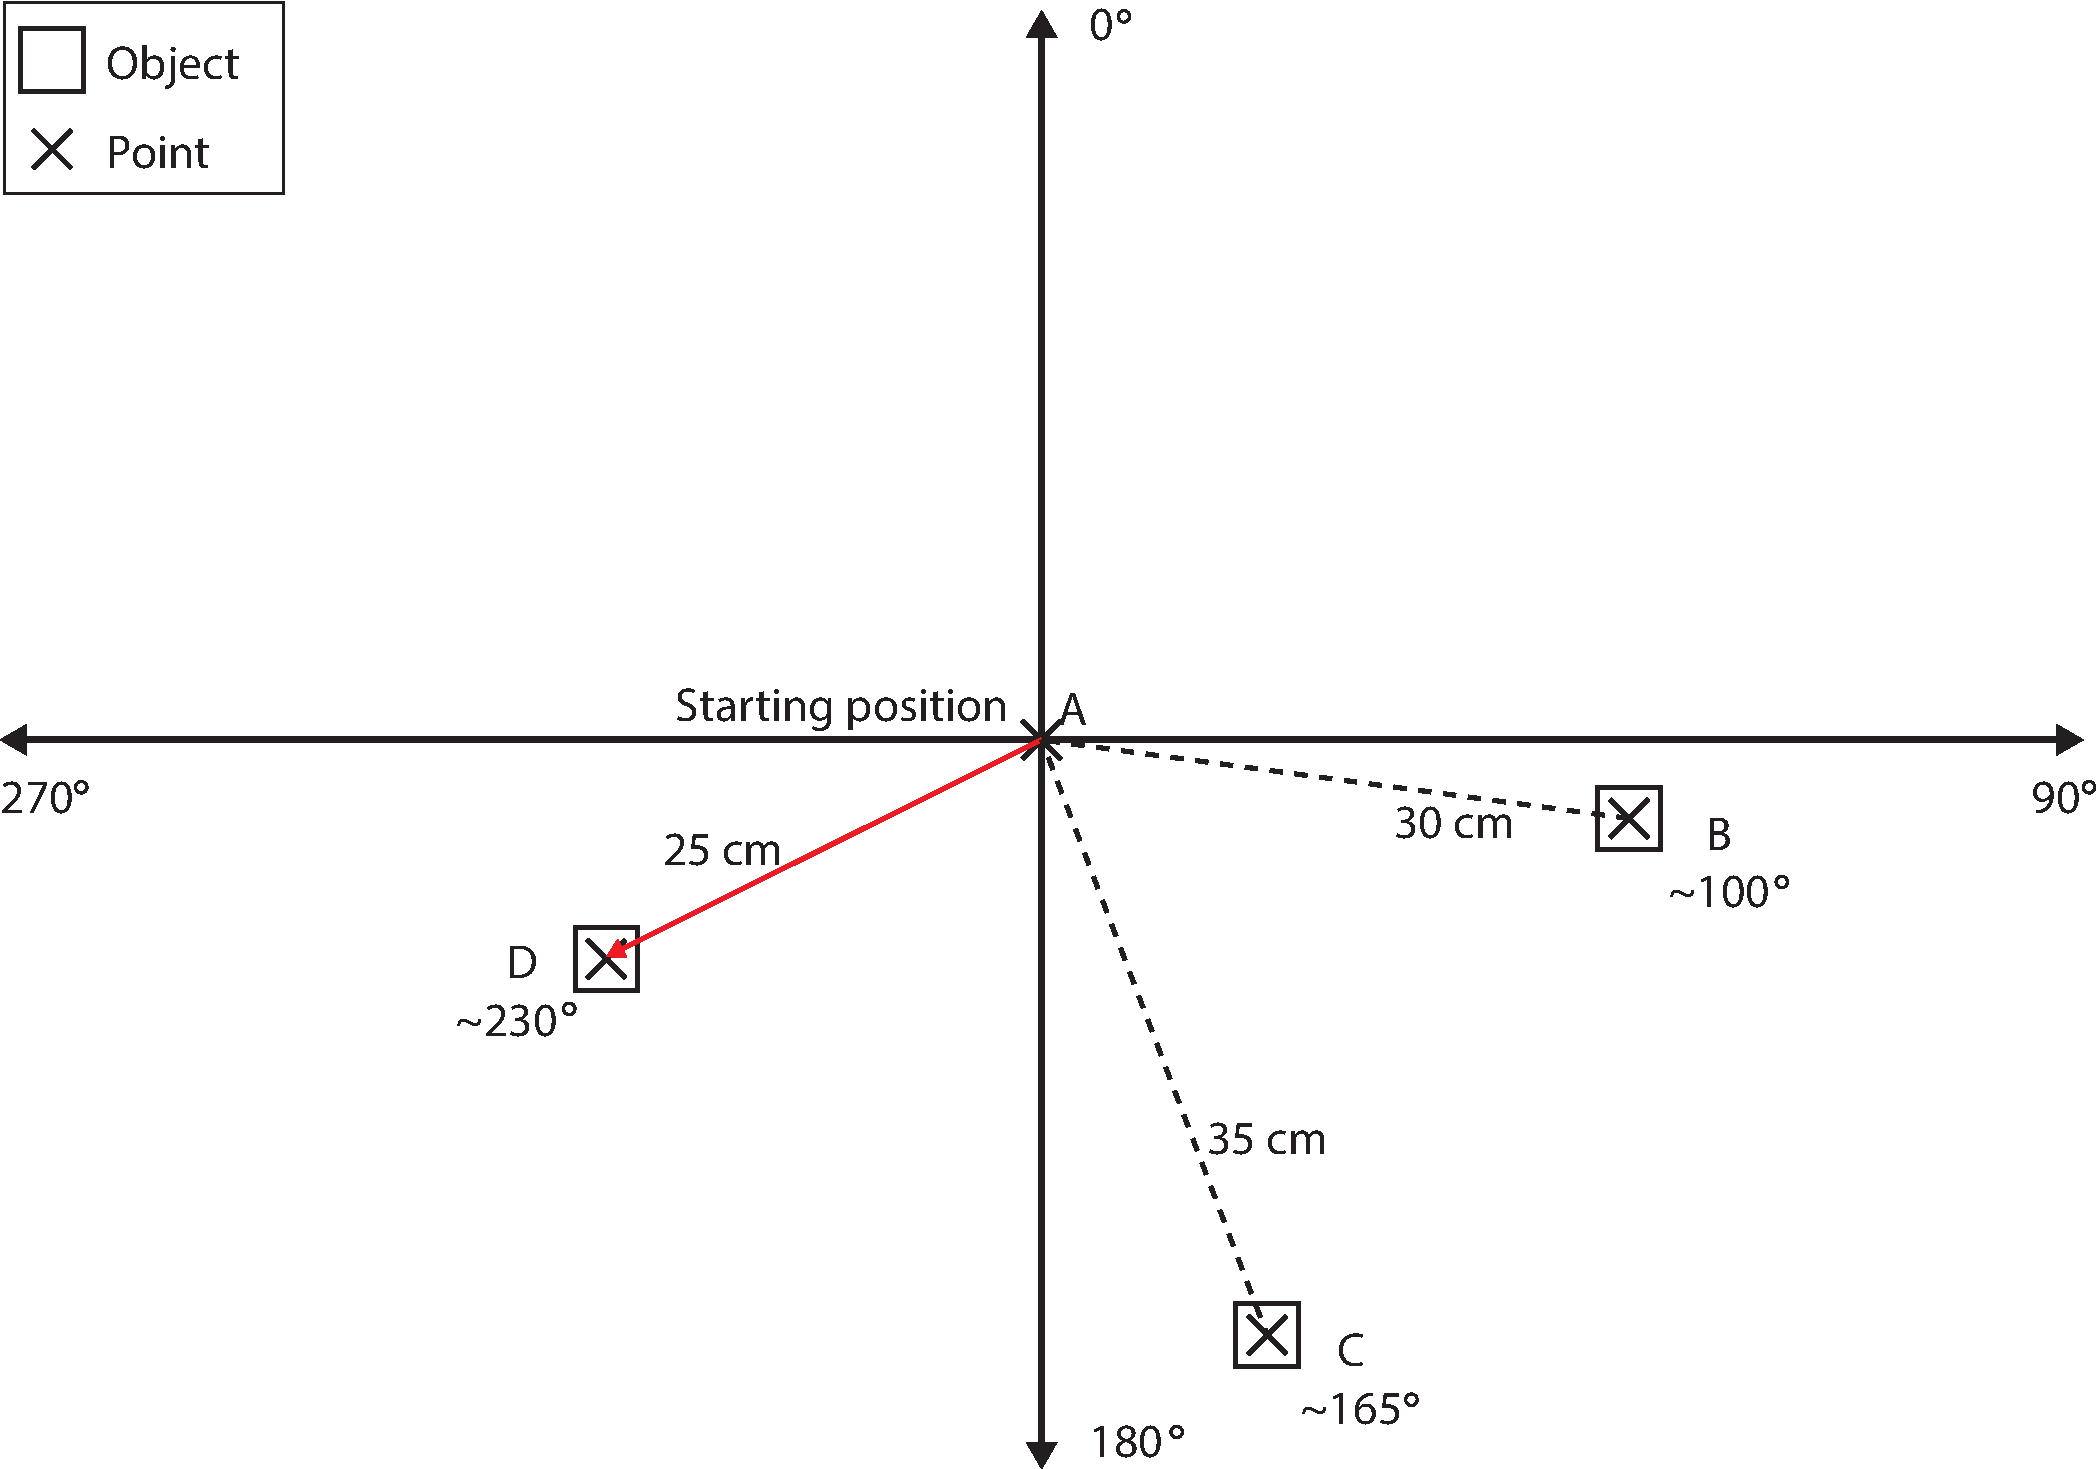
\includegraphics[width=\textwidth]
     {graphics/ObjectNavigationFirst.pdf}}
     \caption{\label{fig:object_navigation_first} First object to be collected.}
\end{figure}

Now that the first object has been scheduled to be collected, the NN-algorithm uses trigonometry to find the shortest distance to the next object, and calculates the angles that is needed to turn, to face the next object. The distance to all the other objects must be calculated, in order to find the closest one. To increase the understanding, the state of the world is represented in \figref{fig:object_navigation_iteration}, where the actions to collect the first object has been applied and reflected in the figure. From this point, the distance to the remaining objects is calculated, using the formula:
\begin{equation}
a = \sqrt{ b^2 + c^2 - 2*b*c*cos(A) } \label{equation:a}
\end{equation}

But for this, the A angle is needed. This is calculated from the spotted angles during the search. The formula for calculating A is:
\begin{equation}
A = (Object~currently~at~spotted~angle) - (Object~closest~spotted~angle) \label{equation:AAngle}
\end{equation}

With the same method as the first object, the object with the shortest distance, from the current object, is found and saves the object number. Now the heading to the closest object must be calculated, and this is the angle calculated by the formula:
\begin{equation}
B = cos^{-1}((a^2 + c^2 - b^2)/(2*a*c)) \label{equation:B}
\end{equation}

This provides the angle that must be turned in order to face the next object. In \figref{fig:object_navigation_iteration} the \projname{} is pointed towards the starting position, and the angle that must be turned is calculated from equation \ref{equation:B}. The current heading added/subtracted (depending on the position) with the angle provides the heading to the next object. This angle is added to the instructions along with the distance. Then the final angle of the triangle is calculated, which is used to turn the \projname{} towards the starting position again. The final angle is calculated with the formula:
\begin{equation}
C = 180 - A - B \label{equation:C}
\end{equation}

In order to point the \projname{} at the starting position again, the current heading is subtracted with (180 - C), where C is found by equation \ref{equation:C}. This process has provided the route to the next object, and the instructions to turn the \projname{} back, facing the starting position. The second step is executed for the remaining objects that were spotted. 

\begin{figure}[H]
     \center{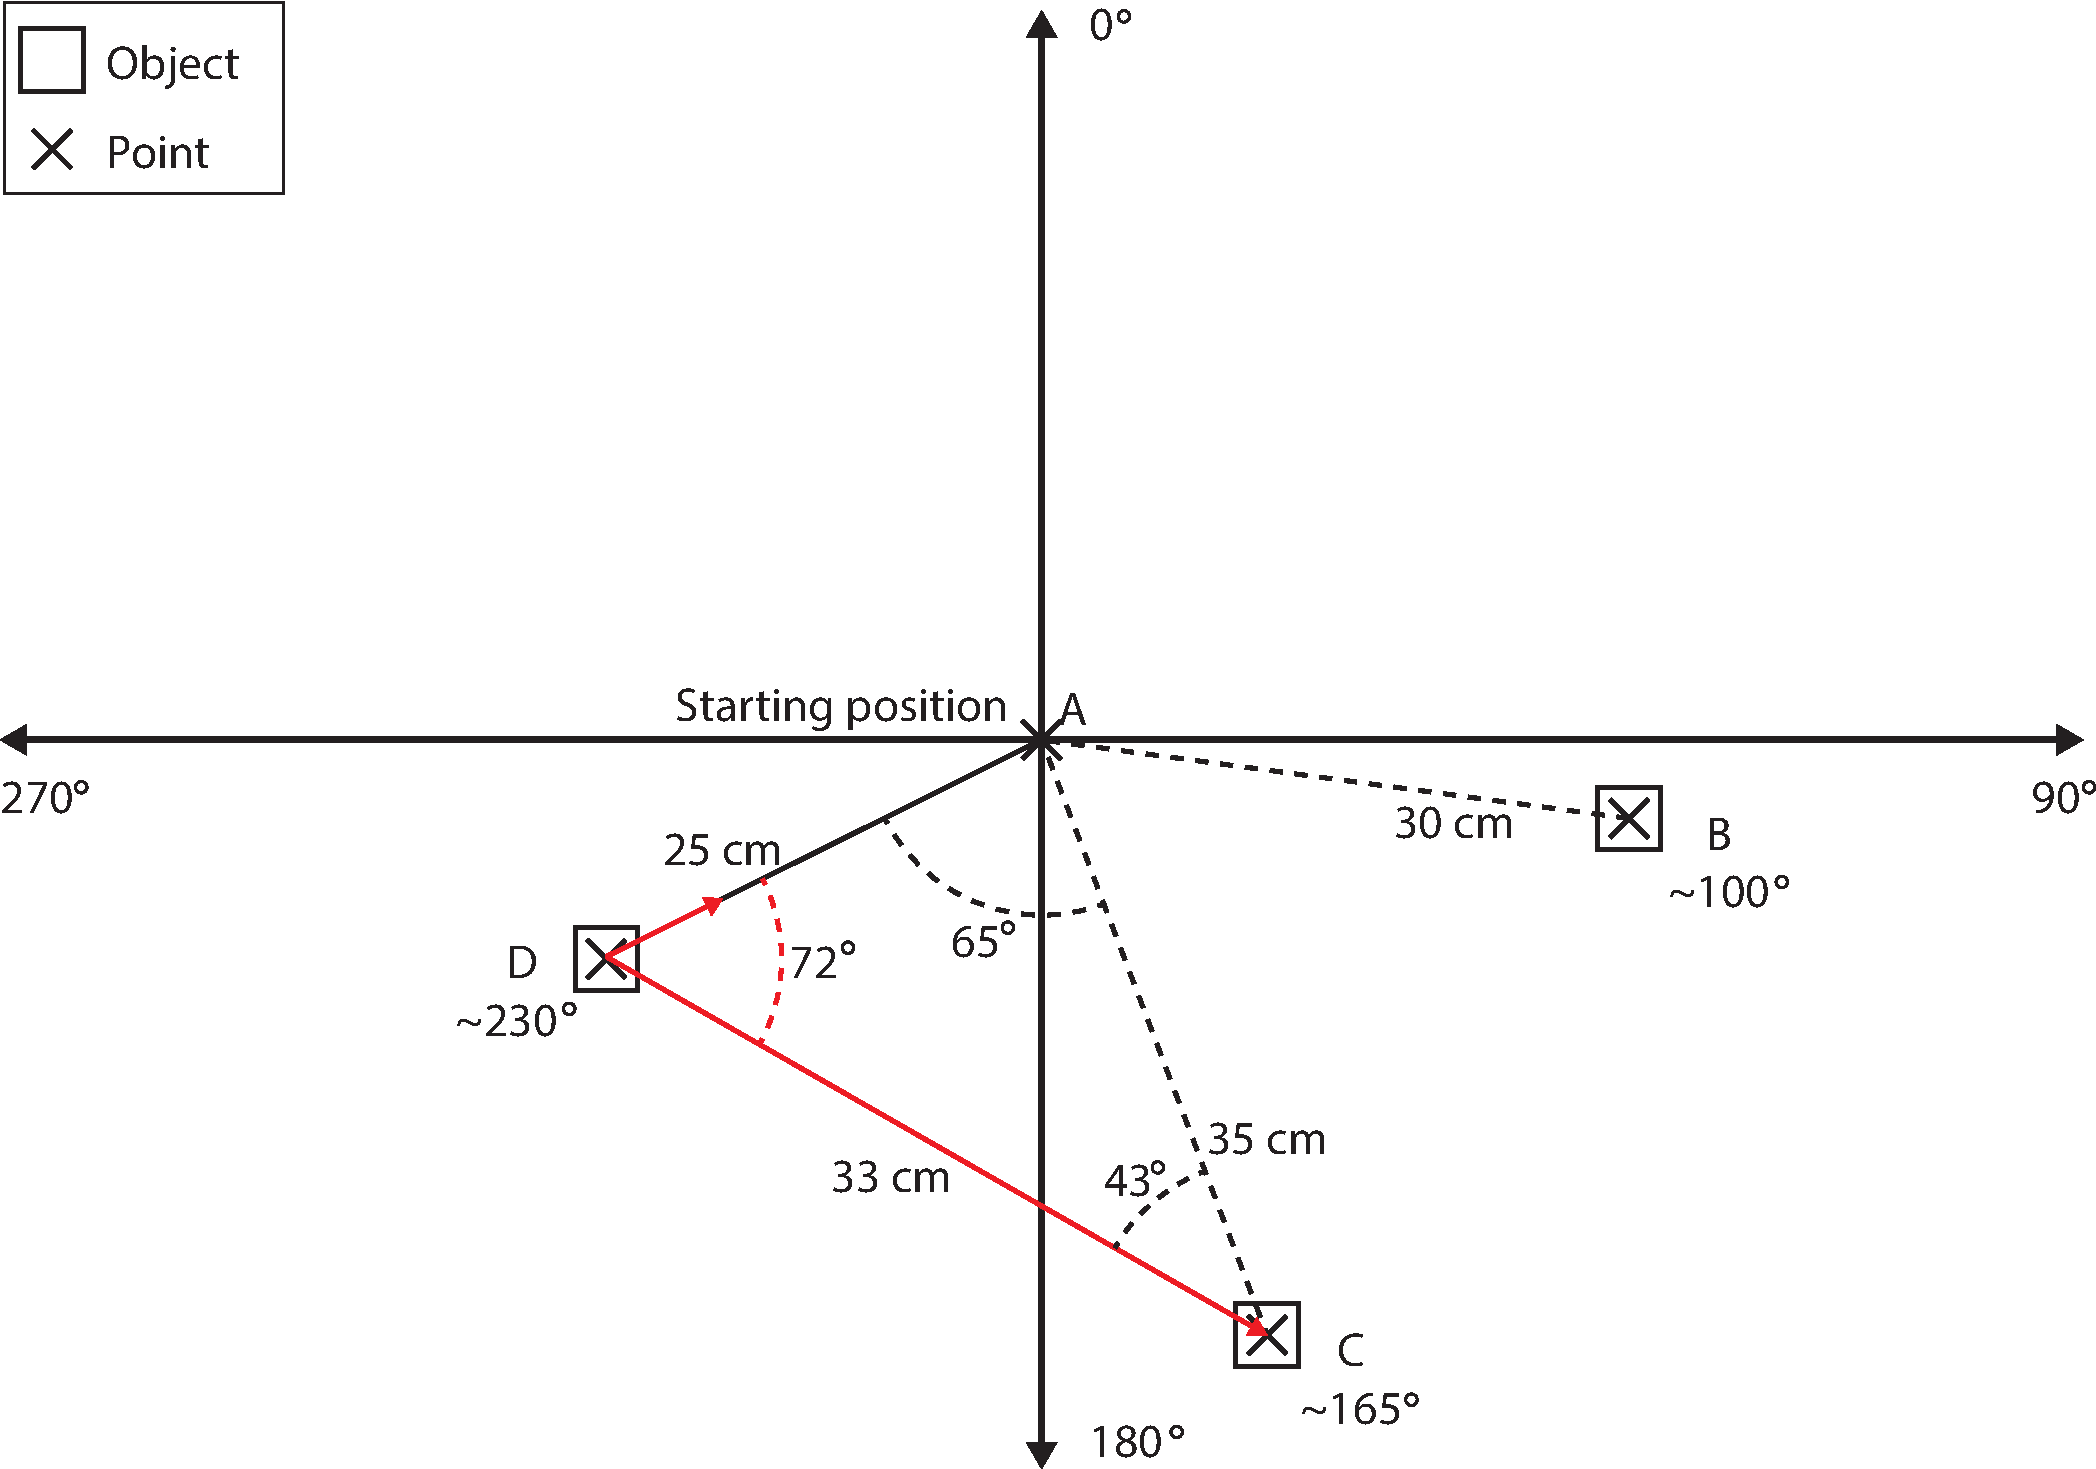
\includegraphics[width=\textwidth]
     {graphics/ObjectNavigationIteration.pdf}}
     \caption{\label{fig:object_navigation_iteration} Iteration of objects to be collected.}
\end{figure}


\subsection{Next-in-view algorithm} \label{sec:niv-algorithm}
An important property of the Next-in-view algorithm, is that it does not do any calculations prior to moving for objects, like the NN-algorithm. However it still relies a lot on the ultrasonic sensor, but in a different way. Instead of using the ultrasonic sensor to map the objects during the initial scan until all objects has been found, it uses the inputs from the sensor until all objects have been collected.

\begin{figure}[H]
     \center{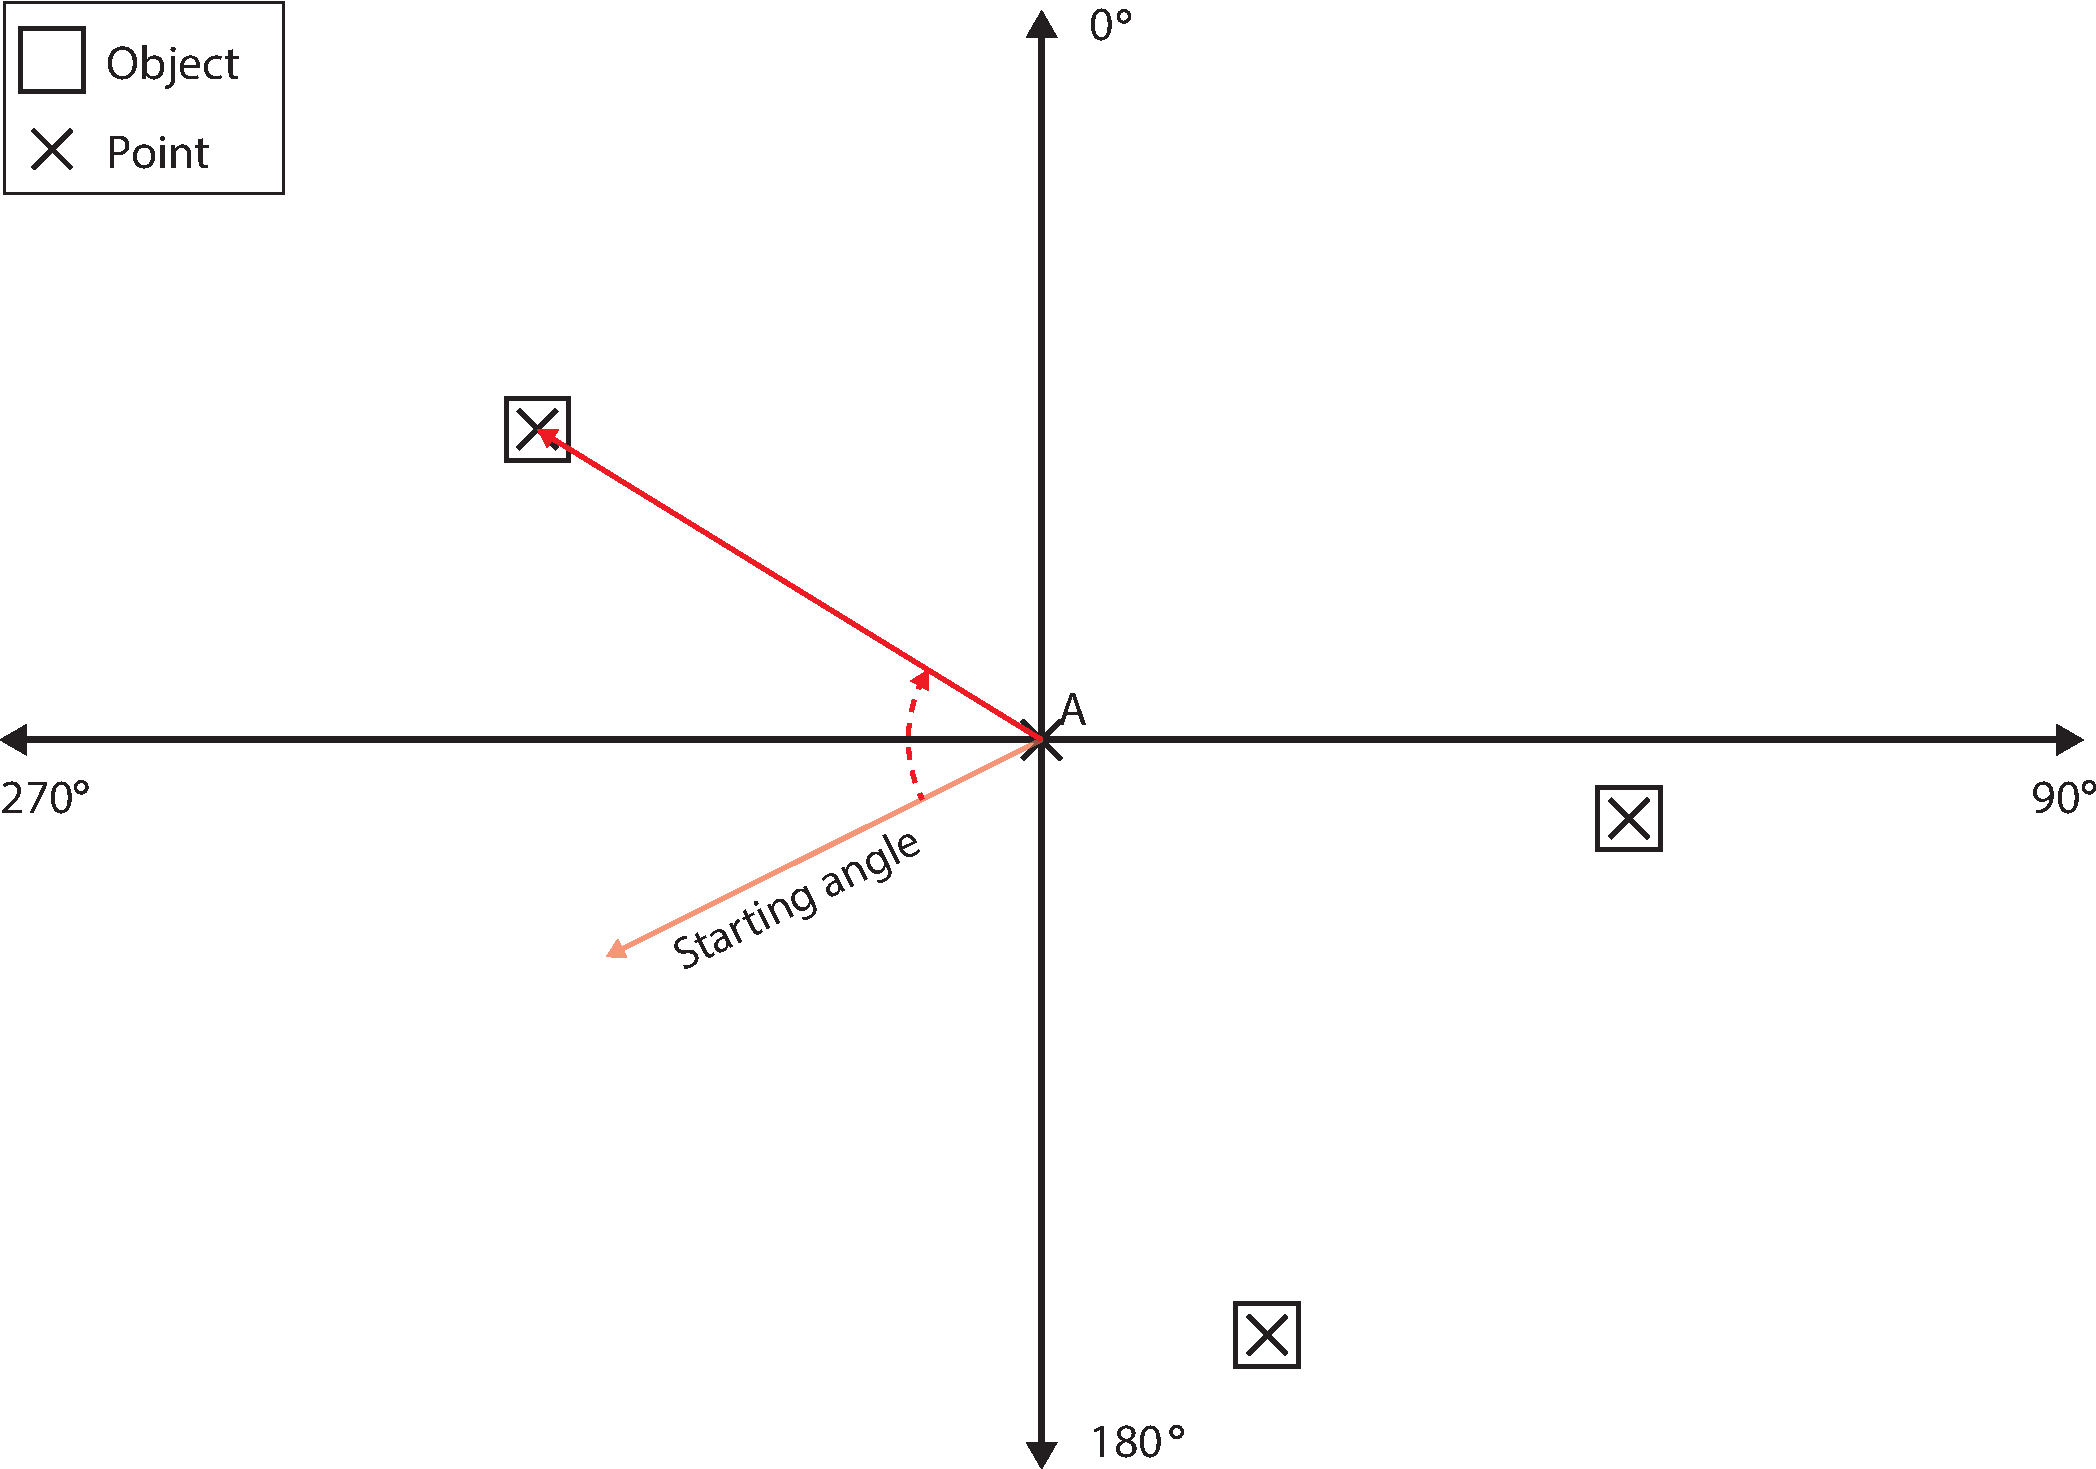
\includegraphics[width=\textwidth]
     {graphics/ObjectNavigationNIV.pdf}}
     \caption{\label{fig:object_navigation_niv} Start-up using the Next-in-view algorithm}
\end{figure}

At start-up the robot starts turning until it spots an object with the ultrasonic sensor, as seen in \figref{fig:object_navigation_niv}. It then drives towards it until the object is within grabbing distance of the claw. The object will be picked up and the \projname{} continues to search for objects, as seen in \figref{fig:object_navigation_niv2}

\begin{figure}[H]
     \center{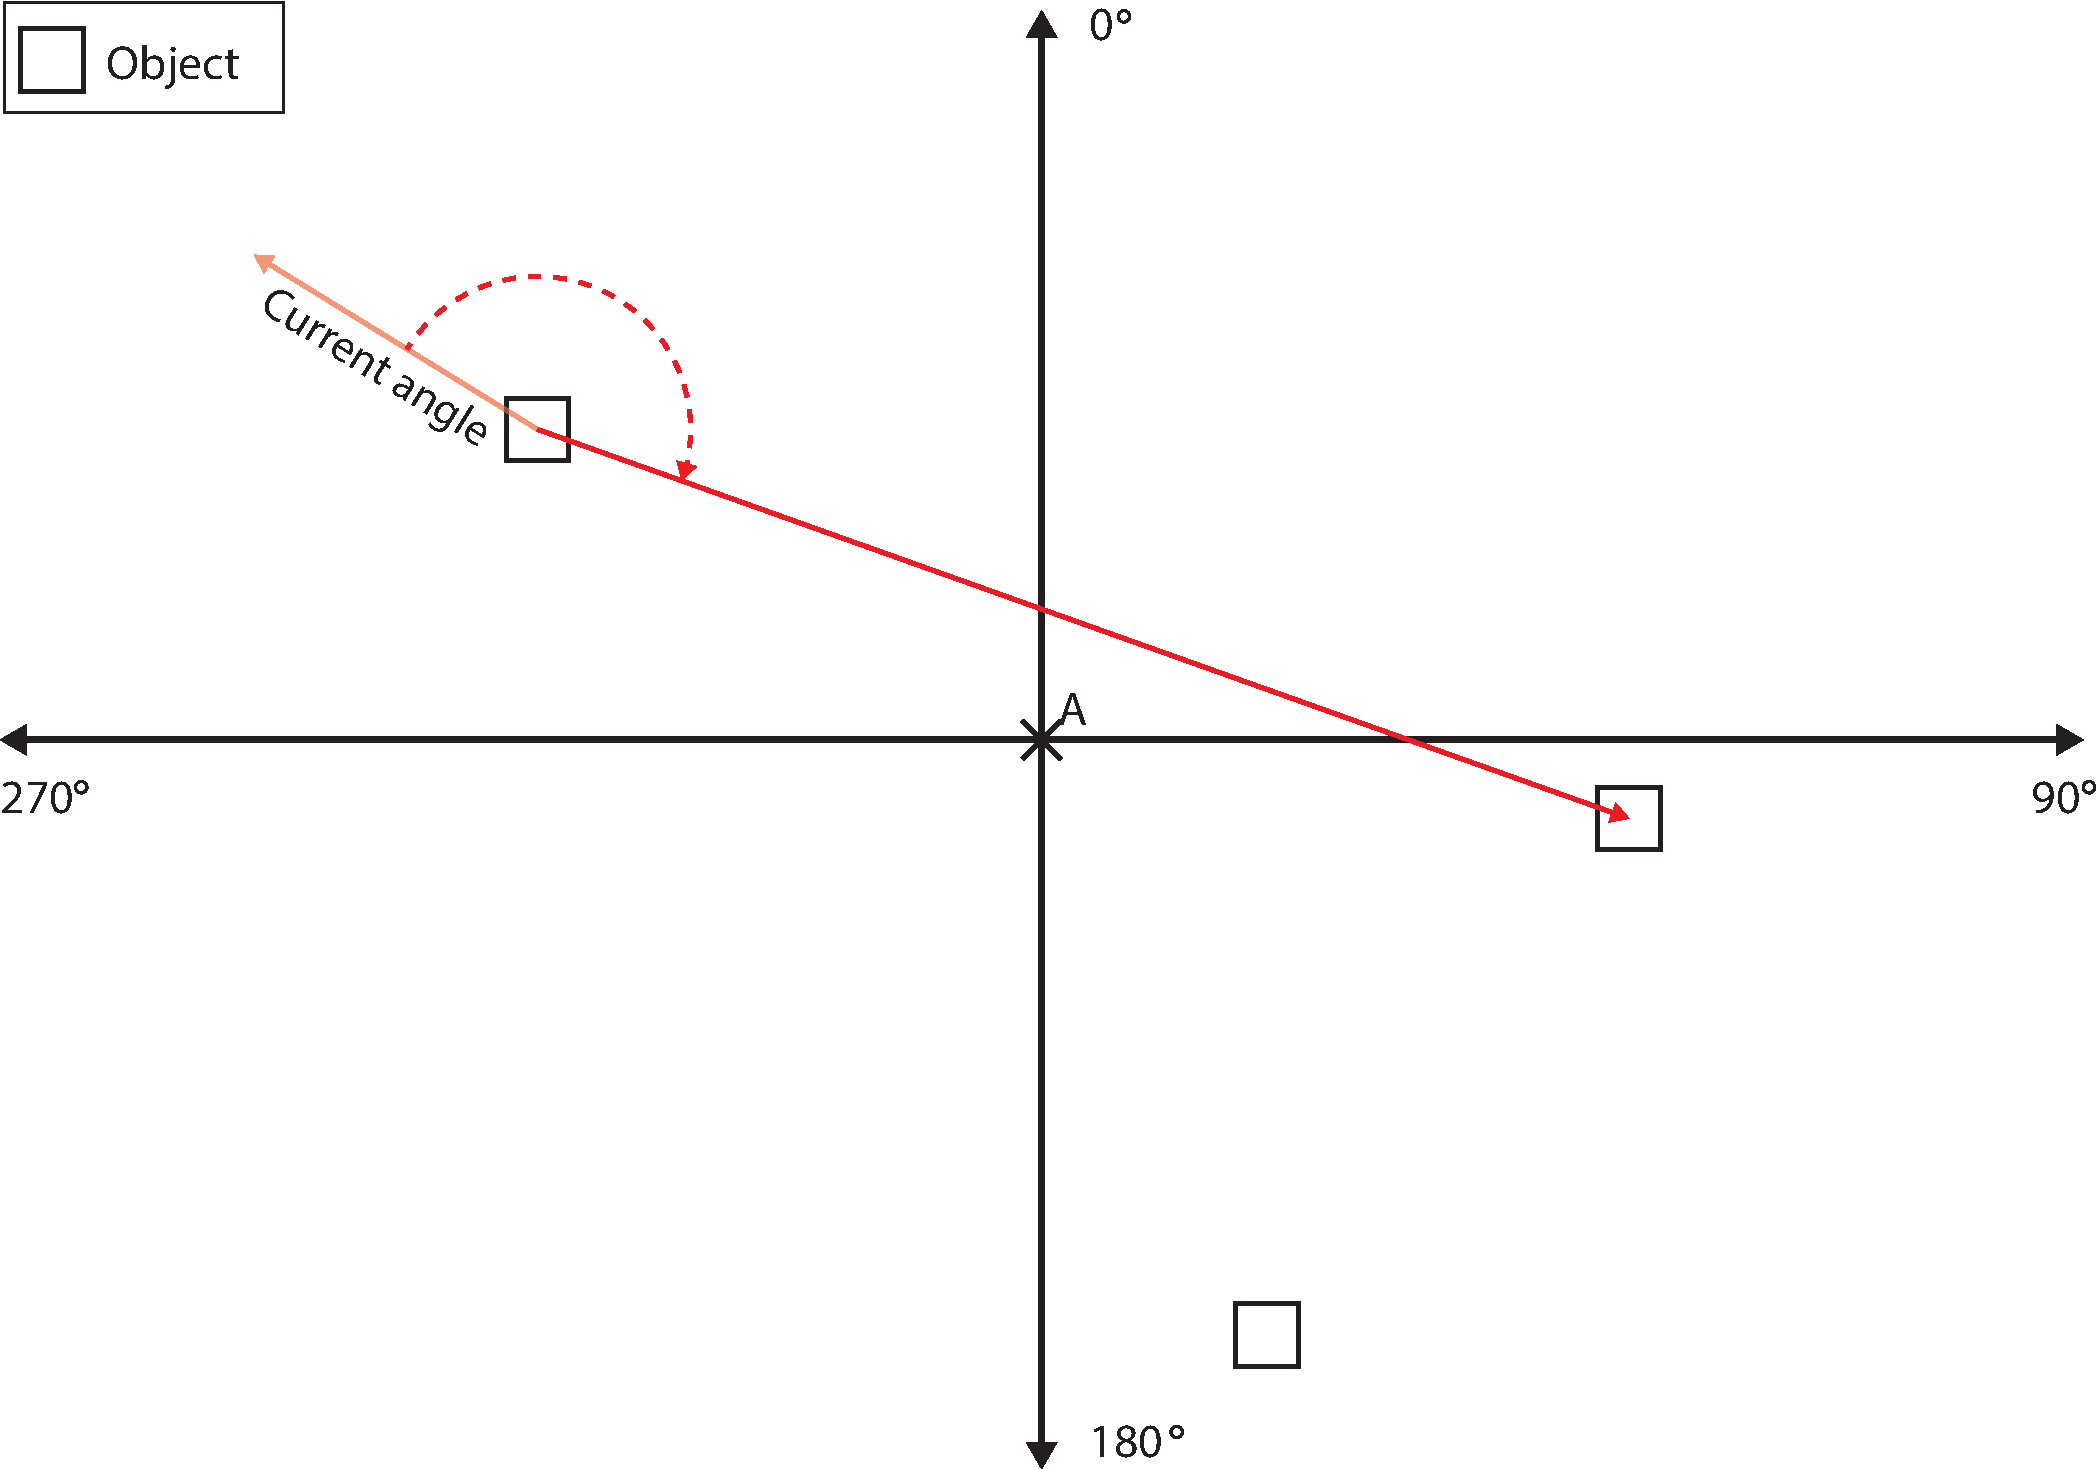
\includegraphics[width=\textwidth]
     {graphics/ObjectNavigationNIV2.pdf}}
     \caption{\label{fig:object_navigation_niv2} Searching for the next object}
\end{figure} 

Because the ultrasonic sensors view is a cone, as described in \secref{sec:hardware}, a case may arise where the robot is not driving straight towards the object. And as it gets closer, it might lose the object as it gets out of the view of the sensor.

In this case, a small routine will be initiated, where the robot will turn a little to the right, followed by a little to the left, constantly scanning for objects, while slowly increasing the angles turned to scan an increasingly larger range. When an object is spotted again, the robot continues to move towards it. When the object has been collected, the robot starts turning until it finds a new object and the entire process continues until every object has been found.


\subsection{Algorithm comparison} \label{sec:algorithm-desc}

The shortest route between the objects can be brute forced by trying out every single possible route between the start position and all of the objects. This would have a calculation time of $\mathcal{O}(n!)$, which means that with every object added, the running time greatly increases. This gives the robot problems when calculating the shortest route, if the amount of objects exceeds a certain number, due to its limited processing power. If there are 9 objects for instance, the number of different paths to check exceeds 360,000.  

A faster, but less distance-efficient algorithm is the NN-algorithm. The algorithm calculates a route based on which objects are closest together. This means that the distance to all the points are calculated from the starting point and the shortest distance is chosen. This is then repeated from the new point, but this time it does not include the objects from previously visited points. This results in a worst case calculation time of $\mathcal{O}(n^2)$, although as the number of remaining objects decreases for each object added to the route, described by $\sum\limits_{i=n}^n i = i - 1$, the calculation time decreases for each object. Compared to the brute force, this algorithm uses only a fraction of the time to compute the result. 

An algorithm that doesn't spend time on calculations prior to moving for objects is the next-in-view algorithm. This algorithm has a number of issues connected to it, which may reduce its performance, however in smaller cases with less than ten objects, its completion speed is close to the NN-algorithm. This is based purely on a theoretical test calculation.

\begin{figure}[H]
     \center{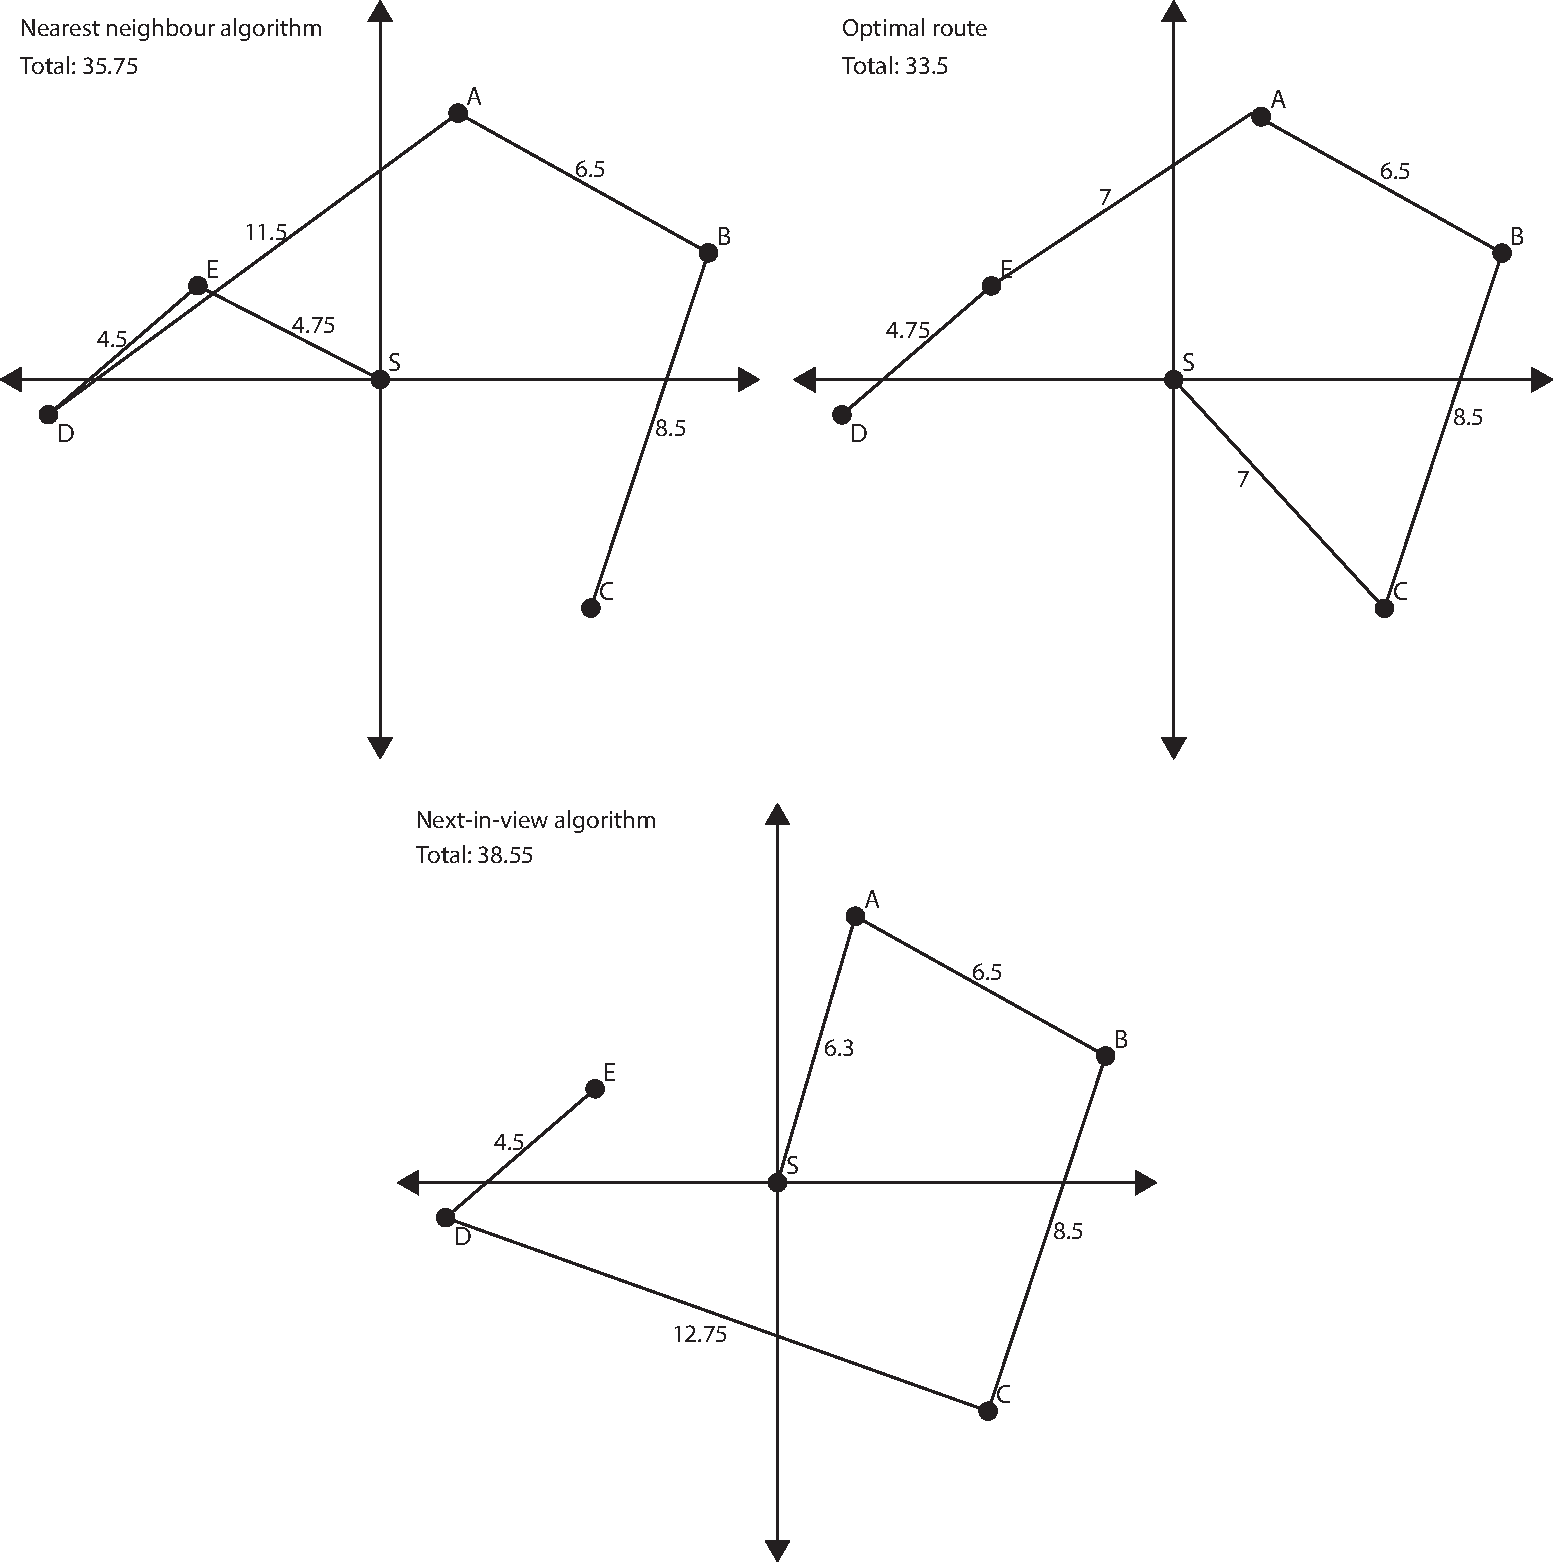
\includegraphics[width=\textwidth]
     {graphics/AlgorithmExamples2.pdf}}
     \caption{\label{fig:algorithm-example} Example of the NN-algorithm, the optimal solution, and next-in-view algorithm.}
\end{figure}

\figref{fig:algorithm-example} shows three solutions to the problem. The top right graph is the optimal solution, which is only used to compare the results from the two other algorithms. Top left is the NN-algorithm, and in the bottom the next-in-view algorithm. The robot starts its route at position \emph{S}. The objects are named in order as they are first detected, if scanning clockwise. The algorithms result in the routes shown on the figure.

The different algorithms result in the routes shown in \figref{fig:algorithm-example}, and have following lengths:
\begin{itemize}
\item Optimal: 33.5 units
\item Nearest neighbour algorithm: 35.75 units
\item Next-in-view: 38.55 units
\end{itemize}

In the average case, the difference between the NN-algorithm and the NIV solutions would be larger if there were more objects to consider. However for these smaller cases, the difference is almost negligible. It should be noted, that this does not describe the time spent, only the distance travelled: rotation to scan for objects, for both algorithms, takes different amounts of time depending on the case. This is not accounted for here.

Due to the limitations of the LEGO NXT brick and the complexity of the problem, finding the optimal solution was ruled out as a possibility. The NN-algorithm maps all objects in the environment, and constructs a route to all the objects before it begins collecting them. The NIV-algorithm is very ad hoc in nature, in that it simply goes for the first object that the robot spots after each scanning cycle is initiated. 

The NN-algorithm is expected to yield the most efficient results, however based on the hardware test of the ultrasonic sensor in \secref{sec:ultrasonic_sensor}, it was deemed unlikely that it would work in practice, since it heavily relies on accurate information about the location of objects in the environment. Due to this, the NN-algorithm was designed in the case that it would work in practice, however the NIV-algorithm was designed and implemented first, as insurance that the robot would be able to complete its task, however not as efficiently.

As mentioned in the test case from \secref{sec:nn-algorithm}, the difference between the two algorithms' distance were nearly insignificant. This also means that using a state-based representation of the world is preferred, where each state represents the robots behaviour. If the NN-algorithm were used, a feature based representation would be better suited for the \projname{}, because of the need to map the location of each found object in relation to the environment.



% Requirement specification
\section{Requirement specification} \label{sec:requirement_specification}

The final version of \projname{} is an autonomous robot that is able to navigate within a marked environment. Within this environment it is able to locate and collect various objects and store them.

\subsection{Requirements}

\projname{} has the following physical features:

\begin{itemize}
    \item \textbf{Tank treads}\\
        Instead of wheels, the \projname{} is equipped with tank treads. This allows the robot to turn around its own axis while not moving away from the position. The tank treads provides the \projname{} with a better grip on a multitude of surfaces.
    \item \textbf{Robotic arm to collect objects}\\
        Consisting of 2 servo motors, this arm has two moveable joints: one to move the arm itself from the front of the \projname{} where it is mounted to the back, and one to control the claw that grabs hold of objects.
    \item \textbf{Sensors to detect objects, environment boundaries and the heading of the robot}\\
        Two colour sensors, one in each front corner. Between those sits an ultrasonic sensor to detect distance. A compass sensor is stably mounted 10 cm above the NXT bricks and at least 15 cm from the motors to avoid any magnetic disturbance.
    \end{itemize}
    
The \projname{} is able to perform the following actions:

    \begin{itemize}
    \item \textbf{Navigate the environment within the boundaries}\\
        The robot is able to move around within the environment, as described in \secref{sec:delimitation}, while searching for objects to collect. If it encounters a boundary, it is able to navigate itself back and find a new direction.
    \item \textbf{Control collection arm to pick up and store objects of specified size}\\
        When an object is detected in the correct position, the \projname{} is able to pick it up and store it, using its motorised arm and claw.
    \item \textbf{Find and collect all objects within reasonable time}\\
        The \projname{} is able to find, collect and store all objects within the environment within the time limit set in \secref{sec:model}.
\end{itemize}





%\subsection{Testing}
%The robot and its functions were tested in various different stages. As in the implementation procedure, the functions were tested individually. The individual functions were then combined one by one while being tested simultaneously, until the robot was fully assembled. The first round of tests can be seen in \secref{sec:hardware} while the final overall test can be found in \charef{cha:quality-assurance}. 

%The final version of \projname{} will consist of a set of tank treads for movement and navigation, a movable arm with a functional claw for grabbing objects, a colour sensor to detect the border of the environment, and a storage container on the back for storing the collected objects. The robot's LEGO components and their functionality can be found in \secref{sec:functionality_description}. The robot will be able to navigate within the environments boundaries and find objects which it will collect and store in its container.


% Implementation
\chapter{Implementation} \label{cha:implementation}

In this chapter, the implementation procedure of the features in \charef{cha:design} are documented, as well as the overall architecture and the choices made in regard to this. The behaviour of the robot is also described, followed by an explanation on how the implemented motor controller works.

%Finally, the finished modules of the \projname{} were listed and documented.

% Implementation procedure
\section{Implementation procedure} \label{sec:imp-procedure}

To implement the features listed in \charef{cha:design}, a stepwise approach was utilised. First, the finished design concept was cut into modules, each with a clearly defined, separate task to accomplish. These modules are what constitutes the final product, however it is possible to implement each of them independently of the others. The modules were ordered according to their importance and relevance to the final product's overall quality, and then tested and implemented in the order seen below.

\begin{enumerate}
\item Basic movement
\item Object collection
\item Bluetooth communication
\item Boundary detection
\item Object detection
\item Basic object navigation
\item Advanced movement
\item Advanced route navigation
\end{enumerate}

This approach made it possible to ensure, that a new feature or module of the robot would only be implemented, when the robot's previously implemented modules are fully operational and complete. This means that each module is known to be working correctly, the challenge is then to combine these. 

This should not be viewed as an absolute approach: work did begin on the next iterations, even if the prior ones weren't finished yet, however it serves well to illustrate how the process was planned and in what order the features were added.

To visualise these modules, a flowchart tool was used to map the different actions and considerations the robot makes when complete. Each added module of functionality was assigned with a new colour to maintain an overview of the iterations. 

\begin{figure}[H]
     \center{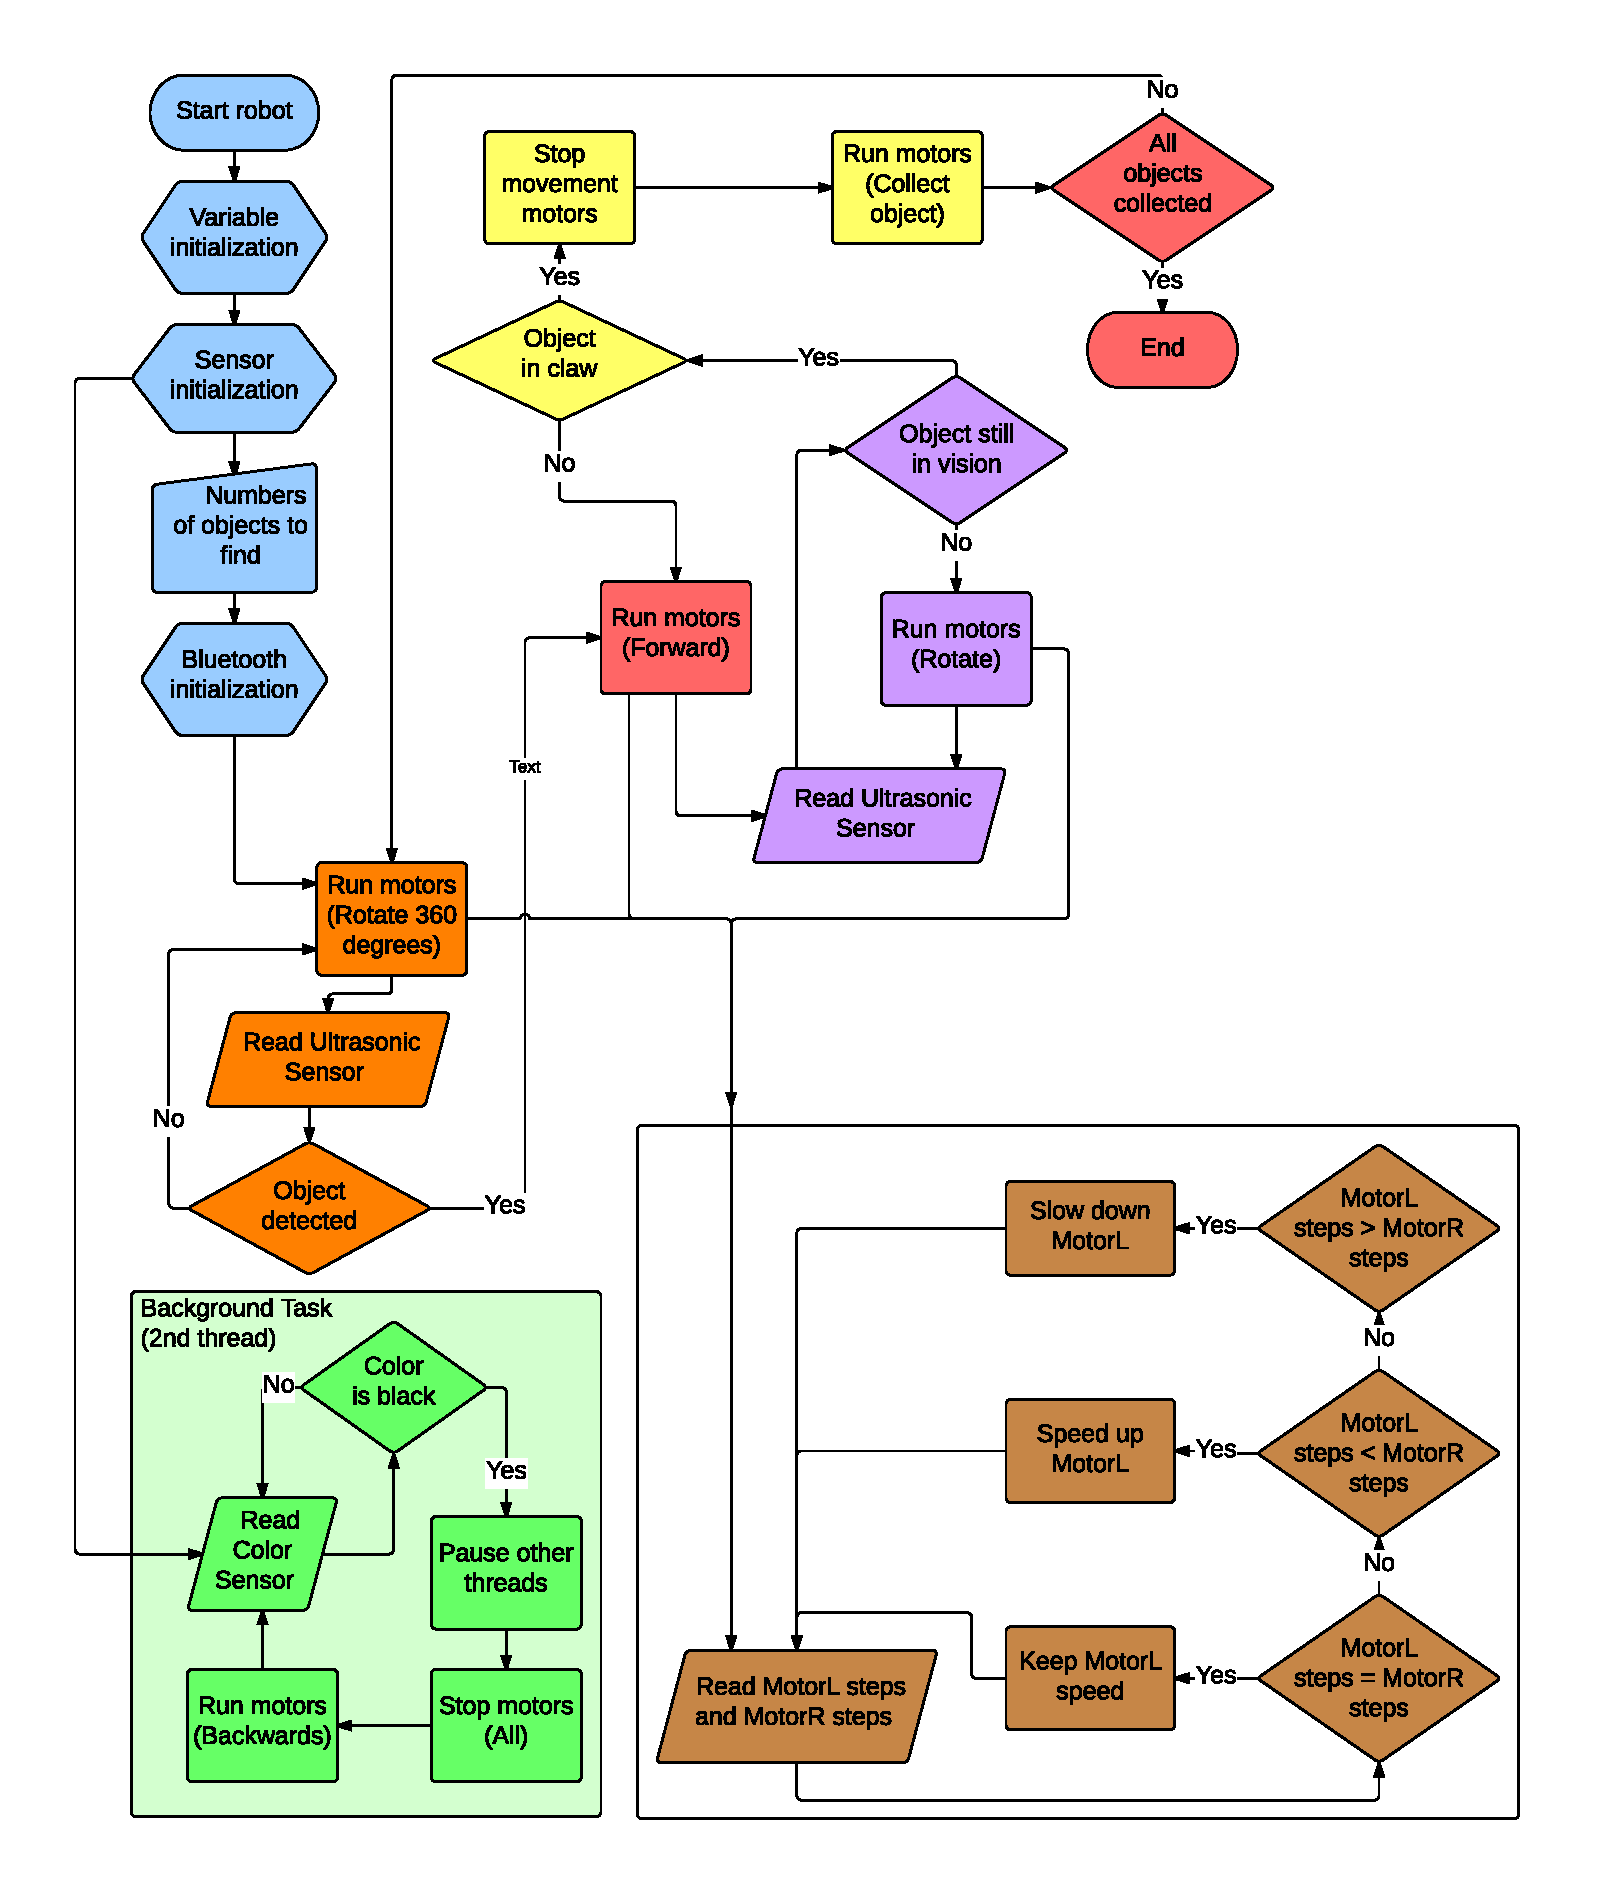
\includegraphics[width=\textwidth]
     {graphics/CompleteRobotFlowchart.pdf}}
     \caption{\label{fig:CompleteRobotFlowchart} Flowchart of the robot and its behaviour.}
\end{figure}
\fxnote{Skal vi tilføje tekst til MC boksen?}

In the diagram in \figref{fig:CompleteRobotFlowchart}, the sections are coloured according to what functionality they fulfil. The previously mentioned iterations often focus on one of the particular partitions of the flowchart. The iterations are described below.


\subsubsection{First iteration --- Basic movement}
In the first iteration, the first module was implemented: the basic movement behaviour. This iteration resulted in a basic robot with tank treads, that could move forward and backwards, and turn left and right around its own vertical axis. The robot, at this point, was able to move around in a square pattern, and end up at the starting location, with an accuracy of a few centimetres. Movement accuracy at this point was hard coded. The blue part in \figref{fig:CompleteRobotFlowchart}, which is the basis for all implementation, was also implemented in this iteration, except for the bluetooth initialisation.


\subsubsection{Second iteration --- Object collection}
In the second iteration, the robotic arm and claw used to collect objects were designed, built and developed. This collection module was tested and tweaked separately, after which it was implemented into the robot itself. This module corresponds to the yellow part in \figref{fig:CompleteRobotFlowchart}.


\subsubsection{Third iteration --- Bluetooth communication}
With the \projname{} being able to move, controlled by one of the NXT brick, and a claw and arm capable of collecting objects controlled by another brick, communication between these two bricks was the next priority to implement. This was done using the inherent Bluetooth-capabilities of the bricks. The master brick sends instructions to the slave brick, and await confirmation from the slave brick, when the task is done. This allowed for the code and behaviour to be centralised on one brick, only communicating simple instructions once in a while over Bluetooth.


\subsubsection{Fourth iteration --- Boundary detection}
This iteration implemented the colour sensors, and made it possible to detect the environment boundaries. This includes functionality to stop, reverse, and turn away from the detected line, searching for new objects. This entire feature runs in a thread by itself. This corresponds to the green part in \figref{fig:CompleteRobotFlowchart}. 


\subsubsection{Fifth iteration --- Object detection}
This iteration included the implementation of basic object detection; the \projname{} is at this point able to turn 360 degrees around while scanning for objects with the ultrasonic sensor. The ultrasonic sensor is able to detect the distance between the robot and the target object. This corresponds to some of the states in the orange part in \figref{fig:CompleteRobotFlowchart}.


\subsubsection{Sixth iteration --- Object navigation}
This iteration focused on implementing the next-in-view algorithm to find and collect objects within the boundary. The routine to find lost objects, as described in \secref{sec:niv-algorithm}, can be seen in \figref{fig:CompleteRobotFlowchart} as the purple part.


\subsubsection{Seventh iteration --- Advanced movement}
During this iteration a motor controller was developed, to ensure that the motors drive alike, in the amount of steps driven. This motor controller is used to drive straight forwards and backwards with greater precision, than the basic movement it replaces. Another motor controller was developed, but this one is used to turn the \projname{} with precision. This motor controller is used to turn a given amount of degrees, or get to a heading, choosing the most relevant turning direction. This feature is shown in the brown part in \figref{fig:CompleteRobotFlowchart}.


\subsubsection{Eight iteration --- Advanced route navigation}
The last iteration was supposed to implement the NN-algorithm described in \secref{sec:nn-algorithm}, but due to the result of the hardware test, it was decided not to implement the NN-algorithm in the final version. The ultrasonic sensor was not able to detect objects with enough precision so that the \projname{} could accurately calculate any useful information based on the data. Due to this limitation, the \emph{next-in-view} algorithm was chosen for implementation. The source code of the NN-algorithm can be found in \appref{app:CD}.


%The hardware problems, primarily the ones caused by the ultrasonic sensor, were too difficult to solve at this point in the project and this iteration will therefore not be implemented in the final program. Instead, the next-in-view algorithm will be the final algorithm. It is possible to see what would have been implemented in \secref{sec:object-navigation}. A comparison between algorithms, and a more detailed explanation of them, can be seen in \secref{sec:algorithm-desc}.

%The blue section, with the \emph{Start robot} node, is the initial start-up phase of the robot. Variables and sensors are initialised, and the number of objects to look for is determined through user input. This is the basis for the implementation. The parts marked in red describe the behaviour of the movement module. The initial implementation of the movement was the ability to move forwards, backwards and to turn left and right with some precision. The yellow part is the object collection behaviour, which handles the movement of the claw and arm that grab hold of and then collect the objects in the environment. After the arm and claw could successfully grab and collect objects, it was implemented into the movement module, to prevent the robot from changing position while an object is being collected.

%Afterwards, the purple part --- the object-detecting half of the scanning module --- was implemented, to allow the robot to actually detect the objects and determine when to activate the collection module. This module also guides the movement module's behaviour, since the movement at this stage is based on where the 

%one brick being the master unit sending instructions, the other being the slave, receiving instructions and returning confirmation. In the case of \projname{}, the brick with the scanners and the movement control was chosen to be the master, and the brick in control of the object collection module the slave. This allowed for the code and behaviour to be centralised on one brick, only communicating simple instructions once in a while over Bluetooth. 

%This iteration focus on implementing a more intelligent way to locate and collect all objects. At this point the robot is able to locate all the visible objects from the starting position. The robot turn 360 degrees and save the angle and distance of all the objects which the robot detects. The \projname{} then navigates to the spotted objects in sequence and attempts to grab these. If the boundary is spotted while driving to a object, then the \projname{} abandons the object, and moves on to the next object. 

%moving towards any object spotted. When it is within sufficient range of the object, it will attempt to pick up the object using the previously implemented collection module. This basic object detection allows the robot to --- in some cases --- complete the intended task successfully.

% Architecture 
\section{Architecture} \label{sec:architecture}
This section focuses on the architecture of the program. Firstly, tasks, events, and alarms used in the \projname{} are discussed. Then follows a number of sequence diagrams, that outlines the function of each task. 


\subsection{Tasks, events, and alarms} \label{sec:task-events-alarms}
This section focuses on the tasks, events, and alarms used in the \projname{}. These are all declared in an OSEK Implementation Language (OIL) specification. All the static declaration of system objects are specified in the OIL file. The OIL specification and the code makes up the program~\citep{nxtOSEK2}. The following subsections focuses on tasks, events, and alarms, what they are and how they are used in the \projname{}.

\subsubsection{Tasks} \label{sec:tasks}
nxtOSEK utilises task to control the program execution, where it is possible to have multiple tasks in one program. There is always a main task from which the primary code is executed. Another common task is one that ensures that certain sensors keeps doing their job. For example if the robot is equipped with colour sensors, the tasks will have to keep pinging the colour sensors which will keep them activated. This sort of task will have to follow a clock to ensure that there is always the same amount of time between each ping to the colour sensor. Each task must be declared in the OIL file. \lstref{lst:taskexample} shows an example of a task declaration, from the \projname{} project. 

\begin{lstlisting}[caption= An example of a task used in the \projname{}, label=lst:taskexample]
TASK MainTask
{
    AUTOSTART = TRUE { APPMODE = appmode1; };
    PRIORITY = 2;
    ACTIVATION = 1;
    SCHEDULE = FULL;
    STACKSIZE = 512;
    EVENT = EventMainTask;
    EVENT = EventSleep;
    EVENT = EventSleepI2C;
};
\end{lstlisting}

The \projname{} contains two tasks: the ``Main'' task, as shown in \lstref{lst:taskexample}, and the ``Background'' task. The Main task contains the primary controls and states of the robot, all within a while loop that keeps the robot going. The Background task is constantly running with two assignments. It keeps pinging the colour sensors background process, to keep them active. Secondly, if a signal has been sent to the slave brick, it waits for the slave brick to respond, when it is done collecting an object. The OS handles which task is executed, depending on the priority of the task. 

\subsubsection{Events} \label{sec:events}
An event, is a trigger, that activates when a certain condition has been met. In nxtOSEK, events can be triggered by an alarm or by signalling the event in the program. An example of an event can be seen in \lstref{lst:eventexample}. The event only has a single attribute, a MASK. This is an integer number, which can be assigned by using AUTO or by manually assigning a number using hexadecimal. The MASK is used to reference the event~\citep{osekoil}. 

\begin{lstlisting}[caption= An example of a task used in the \projname{}, label=lst:eventexample]
EVENT EventMainTask
{
    MASK = AUTO;
};
\end{lstlisting}

\fxnote{Skriv noget om hvordan vi i vores projekt bruger Events}

\subsubsection{Alarms} \label{sec:alarms}
The alarm can be used for a few tasks; activate a task, trigger an event or activate an alarm-callback routine. The alarm is run on a counter, and when this counter has been met, the associated action is performed. An example of an alarm can be seen in \lstref{lst:alarmexample}. The alarm has a few attributes, first there is a COUNTER assigning, where a counter is associated with the alarm. Then the ACTION attribute is set, by describing what ACTION is performed, when the alarm has met its goal. The last attribute is the AUTOSTART attribute, that describes if the alarm action should be triggered at program start~\citep{osekoil}.

\begin{lstlisting}[caption= An example of a task used in the \projname{}, label=lst:alarmexample]
ALARM AlarmMainTask
{
    COUNTER = SysTimerCnt;
    ACTION = SETEVENT
    {
        TASK = MainTask;
        EVENT = EventMainTask;
    };
    AUTOSTART = FALSE;
};
\end{lstlisting}

\fxnote{Skriv noget om hvordan vi i vores projekt bruger Alarms}

% Robot behaviour
\section{Robot behaviour} \label{sec:robot_behaviour}
This section contains a short description of all the available states for the \projname{}. These states are used to determine what process the robot is currently in and to ensure that the robot is always doing as expected.

\begin{description}
\item[Start searching for object] \hfill \\
When the robot is started it will be initialised to this state. In this state the motor settings will be configured for rotating using the default motor speed. After that the \projname{} change state to \emph{Searching for object}.

\item[Searching for object] \hfill \\
In this state the \projname{} continue searching to the right until it finds an object. From this state the robot can go to three different possible states based on the ultrasonic sensor and colour sensors. The ultrasonic sensor always runs in a background task and based on the value form the sensor the \projname{} change state to \emph{Start moving to object}, \emph{Collecting object} or continue in \emph{Searching for object}. If the \projname{} detects black lines the robot will change state to \emph{Start avoiding black line}.

\item[Start avoiding black line] \hfill \\
\emph{Start avoiding black line} configured the motor settings for moving backward. After that the \projname{} change state to \emph{Avoiding black line}. 

\item[Avoiding black line] \hfill \\
\emph{Avoiding black line} start moving the the robot backward until it reach the amount of steps specified in the \emph{Start avoiding black line}. When the amount of steps is reached the \projname{} changes state to \emph{Start avoiding object}.

\item[Start avoiding object] \hfill \\
\emph{Start avoiding object} will setup the motor settings for rotating. After that the robot goes to \emph{Avoiding object}. 

\item[Avoiding object] \hfill \\
\emph{Avoiding object} starts rotating until the ultrasonic sensor cannot see the object anymore. After avoiding the object the robot changes state to \emph{Start searching for object}.

\item[Start moving to object] \hfill \\
This state setup the motor settings for moving forward to the object. After setup the motors the \projname{} change state to \emph{Moving to object}.

\item[Moving to object] \hfill \\
In \emph{Moving to object} the robot start moving forward to the object. From this state the robot can go to two different possible states. If the distance to the object is close the robot will go to \emph{Collecting object}. Otherwise the robot continues moving as long as the ultrasonic sensor detects any object. If the ultrasonic sensor  cannot detect anything the robot will change state to \emph{Start search}.

\item[Collecting object] \hfill \\
In the \emph{Collecting object} state the master sends a message to the slave to collect the object. After this state the robot changes state to \emph{Wait for bluetooth}.

\item[Wait for bluetooth] \hfill \\
In this state the master waits for receiving a message from the slave. When the master had received the message, the robot changes state to \emph{Start searching for object} again. 

\item[Start search] \hfill \\
\emph{Start search} will configured the motor settings for rotate from left to right in small steps. After that the states are changed to Search.

\item[Search] \hfill \\
In the state called \emph{Search} the \projname{} will alternately rotate to left or right. If the \projname{} detects an object on the ultrasonic sensor it will change state to \emph{Moving to object} or \emph{Collecting object}. If the \projname{} do not find any object it will change state to \emph{Searching for object}. 

\end{description}

% Motor controller
\section{Motor controller} \label{sec:motor-controller-imp} 
This section describes the implemented motor controller. As described in \secref{sec:design-motor-controller}, the motor controller repeatedly gets the current amount of steps from the motors and helps the robot drive more accurately. The motor controller makes sure that the robot will drive a certain distance precisely, as well as rotating a certain angle precisely. Furthermore, the implemented speed adjuster will keep the robot driving reliably and compensate for the variety in friction on different surfaces and the motors difference.

The motor controller is implemented using logical expressions in an IF-THEN relationship, usually in the form IF <logical expression> THEN <logical expression>. It can be described using propositional logic. The robot uses a knowledge base to determine what is true about the world, or in this case, about the motors. The motor controller observes the world through the input from the motors and makes decisions on how to change the speed of the motors, based on these observations.


\subsection{Propositional logic}

The propositional logic described below is for moving forward and backwards. The rotation controller is omitted, since it functions alike, though with directional changes. The implemented motor controller is split into the two goals, as described in \secref{sec:design-motor-controller}. 


\begin{equation} \label{eq:motorsteps}
\begin{split}
Motor\_L\_Steps \\
Motor\_R\_Steps
\end{split}
\end{equation}

\begin{equation} \label{eq:motorpower}
\begin{split}
Motor\_L\_Power \\
Motor\_R\_Power
\end{split}
\end{equation}

\begin{comment}
The following $Motor\_\{X\}\_Steps$ variables are values returned from the motors;

\hspace{3mm} $Motor\_L\_Steps$

\hspace{3mm} $Motor\_R\_Steps$

and the $Motor\_\{X\}\_Power$ variables are information given to the motors about how fast they should run.

\hspace{3mm} $Motor\_L\_Power$

\hspace{3mm} $Motor\_R\_Power$

The variable below is the target step to reach for the robot. 

\hspace{3mm} $Target\_Steps$
\end{comment}

It is worth noting that these variables are not Boolean values, but are represented as integers. They are used to determine if speed adjusting is needed or in which direction the robot is moving.

If no speed adjusting is done and no checks are made on if the motors are running equally fast, the robot will not drive straight. Thus, speed adjusting is needed when one motor is ahead of the other in terms of steps. This is illustrated in the following propositions.

\hspace{3mm} $motorR\_ahead \leftarrow Motor\_L\_Steps~<~Motor\_R\_Steps$

\hspace{3mm} $motorL\_ahead \leftarrow Motor\_L\_Steps~>~Motor\_R\_Steps$ 

The atomic proposition $motorR\_ahead$ illustrates if the right motor is ahead of the left motor in terms of steps. If $motorR\_ahead$ is true the motor controller will adjust the speed of the motors such that the left motor, motorL, catches up. The entire compound proposition says, that \textbf{if} $Motor\_L\_Steps~<~Motor\_R\_Steps$, meaning that the number of steps the left motor has run is less than what the right motor has run, then $motorR\_ahead$ is true. Same principle goes for $motorL\_ahead$. 

The following proposition, $moving\_forward$, is similar to the two previous ones, but instead determines which direction the robot is moving, based on what values are sent to the motors. Negative $Motor\_\{X\}\_Power$ values means that said motor is moving forward. This means that if $Motor\_L\_Power < 0 \land Motor\_R\_Power < 0$, meaning both motors are moving forward, then $moving\_forward$ is true. Moving backwards will be referred to using $\lnot moving\_forward$.

\hspace{3mm} $moving\_forward \leftarrow Motor\_L\_Power < 0 \land Motor\_R\_Power < 0$

Now that a basis has been set for determining the robots direction and if speed adjustment is needed, some more propositions can be set up. The rest of the section will describe the actions the speed adjuster performs, as a set of multiple propositional definite clauses. The set of these definite clauses make up the knowledge base the motor controller utilises. All of the definite clauses are on the form $a \leftarrow b$, also known as a rule. The symbol on the left of the arrow is an atomic propersition/an atom and on the right is another atom or a conjunction of atoms.

% Definite clauses for speed adjuster % 
The first of the definite clauses are concerned with speed adjusting. The following two clauses are for the case where the robot is moving backwards. The first clause state that if $\lnot moving\_forward \land motorR\_ahead \land \lnot motorL\_ahead$ then $motor\_power\_increased$ is true. This means that if the robot is moving backwards because $moving\_forward$ is false, the right motor is ahead of the left because $motorR\_ahead$ is true and $motorL\_ahead$ is false, the speed of the left motor will be increased.

\hspace{3mm} $motor\_power\_increased \leftarrow \lnot moving\_forward \land motorR\_ahead \land \lnot motorL\_ahead$ 

The same goes for the second clause. If the robot is moving backwards and the left motor is ahead of the right one then $motor\_power\_decreased$ is true, and the power of the left motor will be decreased.

\hspace{3mm} $motor\_power\_decreased \leftarrow \lnot moving\_forward \land \lnot motorR\_ahead \land motorL\_ahead$

The next two clauses uses the same principles, but here the robot is moving forward. The $motor\_power\_decreased$ and $motor\_power\_increased$ atoms are true under the same conditions as in the previous two clauses.

\hspace{3mm} $motor\_power\_decreased \leftarrow moving\_forward \land motorR\_ahead \land \lnot motorL\_ahead$

\hspace{3mm} $motor\_power\_increased \leftarrow moving\_forward \land \lnot motorR\_ahead \land motorL\_ahead$

% Motor backward, forward and stop
% Definite clauses for destination reached % 
Adjusting the speed of the motors is only one part of the motor controller. The following definite clauses describes how the motor controller ensures, that if the robot is given a distance to drive, it will drive that distance precisely and stop. The motor controller does the same for angles to rotate, but as mentioned previously, the propositional logic for this is omitted because it functions the same way as driving a distance.

As with the case of speed adjusting, before setting up the definite clauses, a few other propositions are needed. The following two propositions determine when the robot is either ahead or behind the target distance. The atom $behind\_target$ is true if either of the motors steps are lower than the target steps. This means that the robot has not yet reached its target distance.

\hspace{3mm} $behind\_target \leftarrow Motor\_L\_Steps~<~Target\_Steps \lor Motor\_R\_Steps~<~Target\_Steps$

The same goes for the next proposition, $ahead\_of\_target$. This will be true if either of the motors steps are higher than the target steps. This means that the robot is past the target distance.

\hspace{3mm} $ahead\_of\_target \leftarrow Motor\_L\_Steps~>~Target\_Steps \lor Motor\_R\_Steps~>~Target\_Steps$

With these propositions set up, the definite clauses for the moving controller can be defined. The following clause state that if neither $behind\_target$ or $ahead\_of\_target$ are true, then $target\_distance\_reached$ is true. This means that if the robot has neither driven too far or not far enough, the robot will stop at this distance, which is the target distance.

\hspace{3mm} $target\_distance\_reached \leftarrow \lnot behind\_target \land \lnot ahead\_of\_target$

The following clause simply states that state that if the target distance has not been reached, $moving\_forward$ will be true, and the robot will move forward.

\hspace{3mm} $moving\_forward \leftarrow behind\_target$

Similar for the last clause states that $moving\_forward$ is false if the robot is past the target distance.

\hspace{3mm} $\lnot moving\_forward \leftarrow ahead\_of\_target$

With this knowledge base, the motor controller could be queried at any point about what is true in the world regarding the motors. The knowledge base is updated live as data are received from the motors. A query could for example be, $target\_distance\_reached$ true? The motor controller would check the knowledge base return an answer. This is essentially what the motor controller is doing in practice, repeatedly checking if some goals have been met.



% Module description
%\section{Module description} \label{sec:module-description}

This section contains a description of the most important modules created for the \projname{}. The entire source code is available in \appref{app:CD}.

\subsection{Bluetooth}
The communication module lets the master and slave unit communicate with each other and transmit values used to determine which operation to perform next. In order to make Bluetooth work, some commands and statements must be executed. First, the necessary initialisations and assignments are required. Then some variables associated with the slave brick is needed in order to establish a connection.

When the connection has been established, is is possible to communicate between the two bricks. From the master unit, the \emph{CallCollectionUnit()} method sends a message to the slave unit. This message tells the slave unit to start the collection process. In the meantime the master unit sits in a while loop and wait for a response from the slave unit, telling it that the unit has been collected and that the master unit can continue its work.

\subsection{Object collecting}
After the bluetooth connection has been established, it is possible to send commands from the master brick to the slave brick. The object collection function is started by the \emph{CallCollectionUnit} method. This starts the \emph{RunCollectUnit()} function, which is run by the slave brick, starting with the claw grabbing the object, the arm moving towards the storage and stopping when it is above it. Then the claw releases the object and go halfway back towards the original position. When it is halfway down it slows down the arm, which increases the motor precision and therefore is able to stop at the exact position instead of a few angles above or below. 

\subsection{Boundary detection}
An important module in the \projname{} is the boundary detection. This is done using two colour sensors. These colour sensors must constantly be pinged, to ensure that they are functioning and ready to provide RGB values. This procedure runs constantly in the background tasked, as described in \secref{sec:task-events-alarms}.

After this, the colour sensors can be used to check the values of the environment, searching for the RGB values associated with the black tape. These RGB values were found when performing the hardware test, described in \secref{sec:colour_sensor}. All these values are defined in the program. There is an \emph{EXTENDED\_RANGE} variable that is applied to all of the minimum and maximum values, to make up for uncertainties. 

Then the values are obtained from the sensors to see whether or not they fit the description of the black tape RGB values. If they do, appropriate commands are performed. The check is run constantly in a loop. The check basically consist of the following: $BlackTapeColourMinValue \leq SensorValue \leq BlackTapeColourMaxValue$, for the colours red, green and blue, for each of the colour sensors. 

\subsection{Objects outside the environment}
But what happens when the \projname{} has detected object outside of the environment and tries to collect these? First of all, when the \projname{} drives towards an objects, and the boundary has been met, the first thing that happens is that the \projname{} drives approximately 15 cm backwards to avoid the black boundary and then make a small turn until the spotted object is no longer in sight. It will then continue its normal 360 degree search and be able to spot new objects again.


%%
% COMMENT
%
\begin{comment}

\subsection{Object navigation}\label{sec:object-navigation}

After all the objects have been spotted, an intelligent route to pick up these is needed. The \projname{} uses the nearest neighbour search (NNS) algorithm to pick up the objects. The algorithm used is shown in \lstref{lst:objectnavigation1} and \lstref{lst:objectnavigation2}. The algorithm looks at the position and distance to all objects, and from the position of the \projname{}, decides what object to pick up first. From the position of the first collected object it decides, from this position, the shortest distance to the next object, and so forth until all the objects are included in the route. 


\subsubsection*{Object navigation --- concept} \label{sec:objnav-concept}
The algorithm uses trigonometry to select the next object, using the object positions observed from the starting positions. The degrees the \projname{} must turn, in order to get to the same heading as the object, is saved as instructions, along with the distance. These instructions must then be followed after the route has been calculated. \figref{fig:object_navigation_first} shows a situation where all the objects have been spotted, and now the \projname{} must decide which object that should be collected first. At this point the shortest object is easy to conclude, as the distance to all objects, from the starting position, is already known. The shortest distance overall is found, and the object associated to this is remembered, and marked as collected, to remove this from consideration when finding the next objects. Then the objects angle and the distance is saved into the instructions array. Another set of instructions is used to ensure that the \projname{} is pointing back, at the starting position. This is used to ease the calculations of the next objects. 

\begin{figure}[H]
     \center{\frame{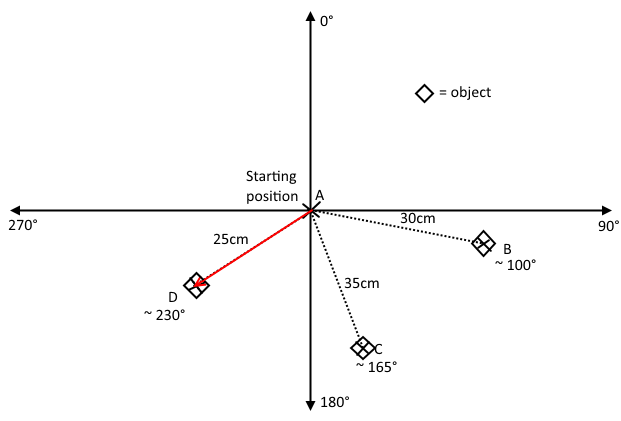
\includegraphics[width=\textwidth]
     {graphics/objectnavigationfirst.png}}}
     \caption{\label{fig:object_navigation_first} First object to be collected.}
\end{figure}

Now that the first object has been scheduled to be collected, the calculations uses trigonometry to find the shortest distance to the next object, and the angles that needs to be turned to face the starting position again. To increase the understanding, the state of the world is represented in \figref{fig:object_navigation_iteration}, where the actions to collect the first object has been applied and reflected in the figure. From this point, the distance to the remaining objects is calculated, using the formula:

\begin{equation}
a = \sqrt{ b^2 + c^2 - 2*b*c*cos(A) } \label{equation:a}
\end{equation}

But for this, the A angle is needed. This is calculated from the spotted angles during the search. The formula for calculating A is:

\begin{equation}
A = (Object~currently~at~spotted~angle) - (Object~closest~spotted~angle) \label{equation:AAngle}
\end{equation}

With the same method as the first object, the object with the shortest distance, from the current object, is found and saves the object number. Now the heading to the closest object must be calculated, and this is the angle calculated by the formula:

\begin{equation}
B = cos^{-1}((a^2 + c^2 - b^2)/(2*a*c)) \label{equation:B}
\end{equation}

This provides the angle that must be turned in order to face the next object. In \figref{fig:object_navigation_iteration} the \projname{} is pointed towards the starting position, and the angle that must be turned is calculated from equation \ref{equation:B}. The current heading added with the angle provides the heading to the next object. This angle is added to the instructions along with the distance. Then the final angle of the triangle is calculated, which is used to turn the \projname{} at the starting position again. The final angle is calculated with the formula:

\begin{equation}
C = 180 - A - B \label{equation:C}
\end{equation}

In order to point the \projname{} at the starting position again, the current heading is subtracted with (180 - C), where C is found by equation \ref{equation:C}. This process has provided the route to the next object, and the instructions to turn the \projname{} back, facing the starting position. The second step is executed for the remaining objects that were spotted. 

\begin{figure}[H]
     \center{\frame{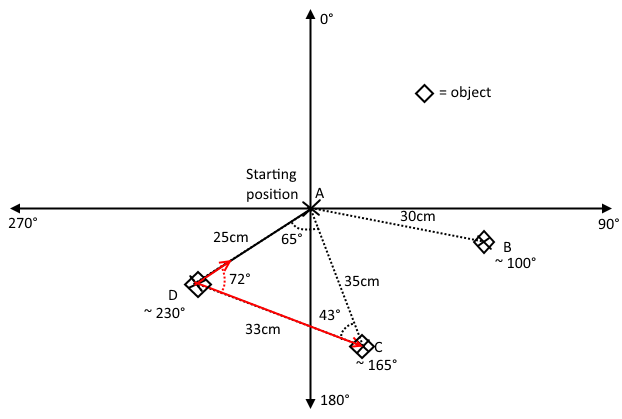
\includegraphics[width=\textwidth]
     {graphics/objectnavigationiteration.png}}}
     \caption{\label{fig:object_navigation_iteration} Iteration of objects to be collected.}
\end{figure}



%
% COMMENT
%
%\begin{comment}
\subsubsection*{Object navigation - implemented} \label{sec:objnav-implemented}

\lstref{lst:objectnavigation1} and \lstref{lst:objectnavigation2} shows the algorithm, as tried to implemented in the \projname{}. It practically works the same way as the concept, but with a few adjustments to make it work. An important little workaround is the boolean \emph{flipped} variable. This is used to decide to which direction, the \projname{} should turn, in order to get to the next object. The problem with choosing the direction is sketched in \figref{fig:choosingdirection}, to help understanding. The difference in angles is calculated, from the object where the \projname{} is currently at. Then angle is checked using the \emph{CalculateValidAngle} function, that ensures that the value is within the possible values (0 - 359). If the difference in angle is bigger than 180, then the flipped variable is set to true, meaning that the turning direction is left, else turn to the right. The \emph{flipped divider}, from \figref{fig:choosingdirection}, shows to which side the \projname{} should turn, depending on which side the object is located. Depending on which side the object is located, different measures to find the angle is used, as shown on in \figref{fig:choosingdirection} This provides us with the correct angle, that should be turned to face the next object. 

\begin{figure}[H]
     \center{\frame{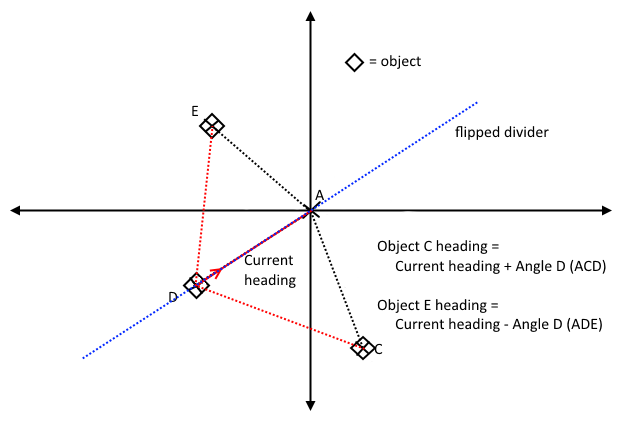
\includegraphics[width=\textwidth]
     {graphics/objnavchoosingdirection.png}}}
     \caption{\label{fig:choosingdirection} Choosing the direction.}
\end{figure}

The algorithm used a boolean array to control which object it has collected, ensuring that the object is removed from the remaining objects, as the \projname{} should only get to each object once. 

The first part of the algorithm can be seen in \lstref{lst:objectnavigation1}. This part shows the initialisation of variables and the input parameters. At line 19, the helper function \emph{FindClosestObjects} is used to find the closest object. Then the case for the first object is shown, where no trigonometry is needed to calculate, as this is from the starting position, knowledge about angle and distance is known from the sensors. 

\begin{lstlisting}[caption= Object navigation start and for the first object, label=lst:objectnavigation1]
void ObjectNavigation(OBJECT objects[], int objectsFound, OBJECT instructions[], OBJECT turnToStartInstructions[])
{
	int addedToRoute = 0;
	int previousObjectNumber = 0;
	int closestObjectNumber = 0;
	S16 currentHeading = compass.getHeading(); 
	bool hasBeenAdded[objectsFound];
	bool flipped = false; 
	
	for (int j = 0; j <= objectsFound; j++)
	{
		flipped = false; 
		closestObjectNumber = findClosestObjects(objects, objectsFound, addedToRoute, previousObjectNumber,  hasBeenAdded);
		
		if (j == 0)
		{
			instructions[j].angle = objects[closestObjectNumber].angle;
			currentHeading = objects[closestObjectNumber].angle;
			instructions[j].distance = objects[closestObjectNumber].distance;
			hasBeenAdded[closestObjectNumber] = true;
			
			previousObjectNumber = closestObjectNumber;
			turnToStartInstructions[j].angle = CalculateValidAngle(currentHeading, 180);
			currentHeading = turnToStartInstructions[j].angle;
			addedToRoute++;
		}
\end{lstlisting}

\lstref{lst:objectnavigation2} shows the case for the n'th object. The difference here is the use of trigonometry to calculate the next angle to turn and distance to travel. Mathematical concepts presented in \secref{sec:objnav-concept} is used to calculate the angles and distances. 

\begin{lstlisting}[caption= Object navigation n'th object, label=lst:objectnavigation2]
		else if (j > 0)
		{
			int b = objects[closestObjectNumber].distance;	
			int c = objects[previousObjectNumber].distance;
			int aAngle = CalculateValidAngle(objects[previousObjectNumber].angle, -objects[closestObjectNumber].angle);
			if (180 < aAngle && aAngle <= 359)
			{
				flipped = true;
			}
			int a = static_cast<int>(sqrt(pow(b, 2)+pow(c, 2)-2*b*c*cos((aAngle*PI)/180)));
			int bAngle = static_cast<int>(acos((pow(a, 2)+pow(c, 2)-pow(b, 2))/(2*a*c)) * 180 / PI);
			int cAngle = ((180 - aAngle) - bAngle);

			instructions[j].angle = (flipped == false) ? (currentHeading+bAngle) : (currentHeading-bAngle);
			instructions[j].distance = a;
			hasBeenAdded[closestObjectNumber] = true; 
			previousObjectNumber = closestObjectNumber;
			turnToStartInstructions[j].angle = (flipped == false) ? CalculateValidAngle(currentHeading, (180-cAngle)) : CalculateValidAngle(currentHeading, -(180-cAngle));
			currentHeading = turnToStartInstructions[j].angle;
			addedToRoute++;
		}
	}
}
\end{lstlisting}


The algorithm uses a function to help find the closest object. This is used to divide the task to increase readability. The \emph{FindClosestObject}, seen in \lstref{lst:findclosestobject}, takes all the objects as input, an array to check which object has been added and knowledge about the last object that was chosen. From this, it checks the objects, those that has not already been added, from the last objects location. The last objects location is the starting position for the first object. The distance to all the other remaining objects is then calculated and the object closest is chosen and returned. 

\begin{lstlisting}[caption= Function findClosestObject, label=lst:findclosestobject]
int FindClosestObjects(OBJECT objects[], int objectsFound, int addedToRoute, int previousObjectNumber, bool hasBeenAdded[])
{
	int closestObjectNumber = -1; 
	int tempDistance = 2000; 
	
	for (int i = 0; i <= objectsFound; i++)
	{
		if (addedToRoute == 0)
		{
			if (objects[i].distance < tempDistance)
			{
				tempDistance = objects[i].distance;
				closestObjectNumber = i;
			}
		}
		
		else if (addedToRoute > 0 && hasBeenAdded[i] == false)
		{
			int b = objects[i].distance;
			int c = objects[previousObjectNumber].distance;
			int aAngle = objects[previousObjectNumber].angle - objects[i].angle;
			if ( aAngle < 0 )
			{
				aAngle = -aAngle;
			}
			int a = static_cast<int>(sqrt(pow(b, 2)-pow(c, 2)-2*b*c*cos((aAngle*PI)/180)));
			
			if ( a < tempDistance )
			{
				tempDistance = a;
				closestObjectNumber = i;
			}
		}
	}
	return closestObjectNumber;
}
\end{lstlisting}

Despite several tests and number tweaking within the algorithm, the problems with the ultrasonic sensor, see \secref{sec:ultrasonic_sensor}, were too severe to get the initial search to work. The sensor were not able to spot the right amount of objects and the precision of the objects were not correct, which resulted in a calculated route that would not hit the objects. It was therefore decided to use the next-in-view algorithm as described in the sixth iteration in \secref{sec:imp-procedure}.
\end{comment}
%
% COMMENT
%
%%The motor controller is split up into two parts: one part for rotation and one part for moving forward and backward. Both part have a function for adjusting the speed and stop the motors on the target angle or step. Only the code for the moving forward and backwards is include in this section, as the code only has small differences.

%The code in \lstref{lst:speed-adjuster1of2} shows the first part of the function to adjust the speed when the robot is moving forward and backwards. This part calculates the min and max steps, that both motors has to be inside. The if-else check ensures that the speed is not set too low or high, else provides a minimum or maximum value for the motors. 

%The second part of the speed adjust code is shown in \lstref{lst:speed-adjuster2of2}. Line 1 checks if the current number of steps for the left motor is inside the min/max range. If that is the case, then the speed adjuster does nothing, and returns the current speed. If the amount of steps is outside the min/max range, line 5 and 16 checks whether the speed should be increased or decreased. 

%\lstref{lst:motor-controller} shows the function to check whether or not the \projname{} has reached the targeted amount of steps. Line 9 and 14 checks which way the \projname{} must move in order to reach the target. If the target is reached the else at line 19 stops the motors.


% Algorithm description
%\subsection{Algorithm description} \label{sec:algorithm-desc}

After the \projname{} has completed its initial 360 degree search and stored the information about the nearby objects, it is time to calculate a route between said objects. Due to the limited power and calculation speed of the LEGO NXT brick it is necessary to find an efficient algorithm that is fast and does not take a lot of computational power and space. 

The shortest route between the object can be brute forced by trying out every single possible route between the start position and all of the objects. This would have a calculation time of $\mathcal{O}(n!)$, which means that every object added greatly increases the running time. This gives the robot problems when calculating a shortest route, if the amount of objects exceed a certain number. If there are 9 objects, the number of different paths to check exceeds 360000. 

A more time efficient, but less effective, algorithm is the NN-algorithm. The algorithm calculates a route based on which objects are closest together. This means that the distance to all the points are calculated from the starting point and the shortest distance is chosen. This is then repeated from the new point, but this time it does not calculate from any previously visited points.

A very simple algorithm, that uses very little calculation, is the next-in-view algorithm. This was the first algorithm to be implemented on the \projname{} due to its simplicity. With this algorithm, the robot starts turning towards either right or left, stopping at the first object it detects. It then moves out to collect this object, and then starts turning towards the same direction again, thus always picking up the next object that comes into its view, hence the name of the algorithm. This algorithm has a number of issues connected to it, which may reduce its performance, however in smaller cases with less than ten objects, its completion speed is close to the NN-algorithm.

\begin{figure}[H]
     \center\frame{{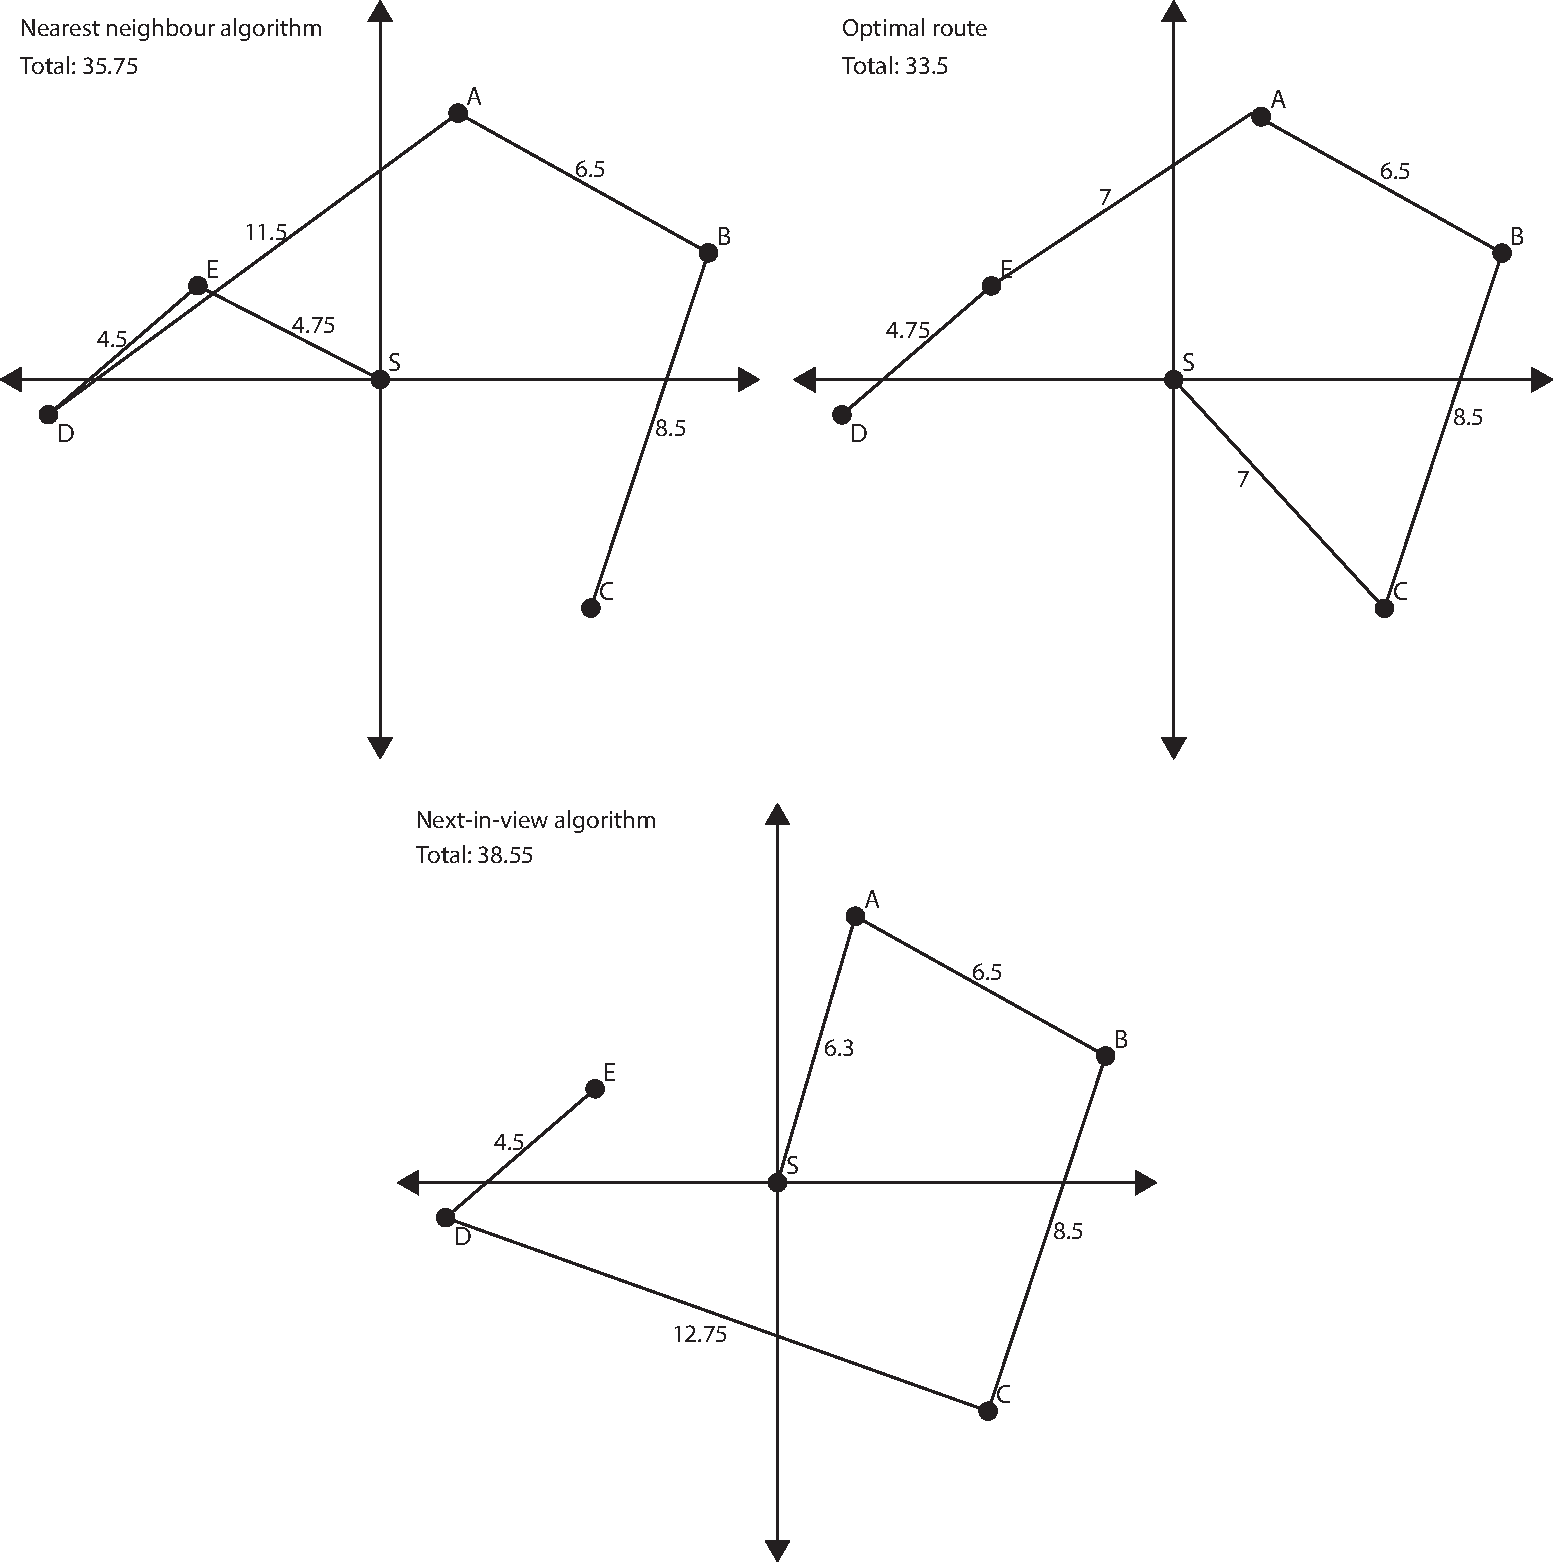
\includegraphics[width=\textwidth]
     {graphics/AlgorithmExamples2.pdf}}}
     \caption{\label{fig:algorithm-example} Example of the NN-algorithm, the optimal algorithm, and next-in-view algorithms.}
\end{figure}

\figref{fig:algorithm-example} shows three solutions to the problem. The top right graph is the optimal solution, which is only used to compare the results from the two other algorithms. Top left is the NN-algorithm, and in the bottom the next-in-view algorithm. The robot starts its route at position \emph{S}. The objects are named in order as they are first detected. The algorithms result in the routes shown on the figure.

The different solutions in \figref{fig:algorithm-example} have following lengths:
\begin{itemize}
\item Optimal: 33.5 units
\item NN-algorithm: 35.75 units
\item Next-in-view: 38.55 units
\end{itemize}

In the average case, the difference between the NN-algorithm and the next-in-view solutions would be larger if there were more objects to consider. However for these smaller cases, the difference is almost negligible. It should be noted, that this does not describe the time spent, only the distance travelled: rotation to scan for objects, for both algorithms, will also take different amounts of time depending on the case. This is not accounted for here.

Due to the limitations of the LEGO NXT brick and the complexity of the problem, finding the optimal solution was ruled out as a possibility. Instead, the NN-algorithm was initially selected to calculate the route for the \projname{}. This algorithm does not always result in the most optimal route, but when the calculation speed and actual running speed is considered, it is arguably faster in the average case. However, as previously mentioned, this algorithm was not implemented. This was the result of inaccurate hardware: the ultrasonic sensor was not able to detect objects with enough precision, that the \projname{} could accurately calculate any useful information based on the data.

Due to this limitation, the \emph{next-in-view} algorithm was chosen for implementation. The simplicity of the algorithm, as well as the fact that it takes the inaccurate sensor input into account, made it the obvious choice. And as previously mentioned in \secref{sec:nn-algorithm}, the distance difference of the two algorithms are nearly insignificant.



% Test
\chapter{Test} \label{cha:quality-assurance}

In this chapter the functionality of the final robot will be tested and described. In relation to the specified requirements in \secref{sec:requirement_specification}, all the requirements is tested. The tests show whether or not the robot is able to perform the actions from the requirements. It is not possible to test the physical features but they have been fulfilled.

The requirements for the robot: 
\begin{itemize}
\item Navigate the environment within the boundaries.
\item Control collection arm to pick up and store objects of specified size.
\item Find and collect all objects within the time limit.
\end{itemize}

\section{Test setup}
To test the \projname{} and its ability to fulfil the three requirements, a testing area similar to a real world environment was set up. This area was determined by a boundary which the robot was not allowed to cross, objects outside the boundary to test the boundary detection, and a certain amount of objects with a size and weight that the robot has proven in \secref{sec:object_specification} to be able to find and collect.

\begin{figure}[H]
     \center{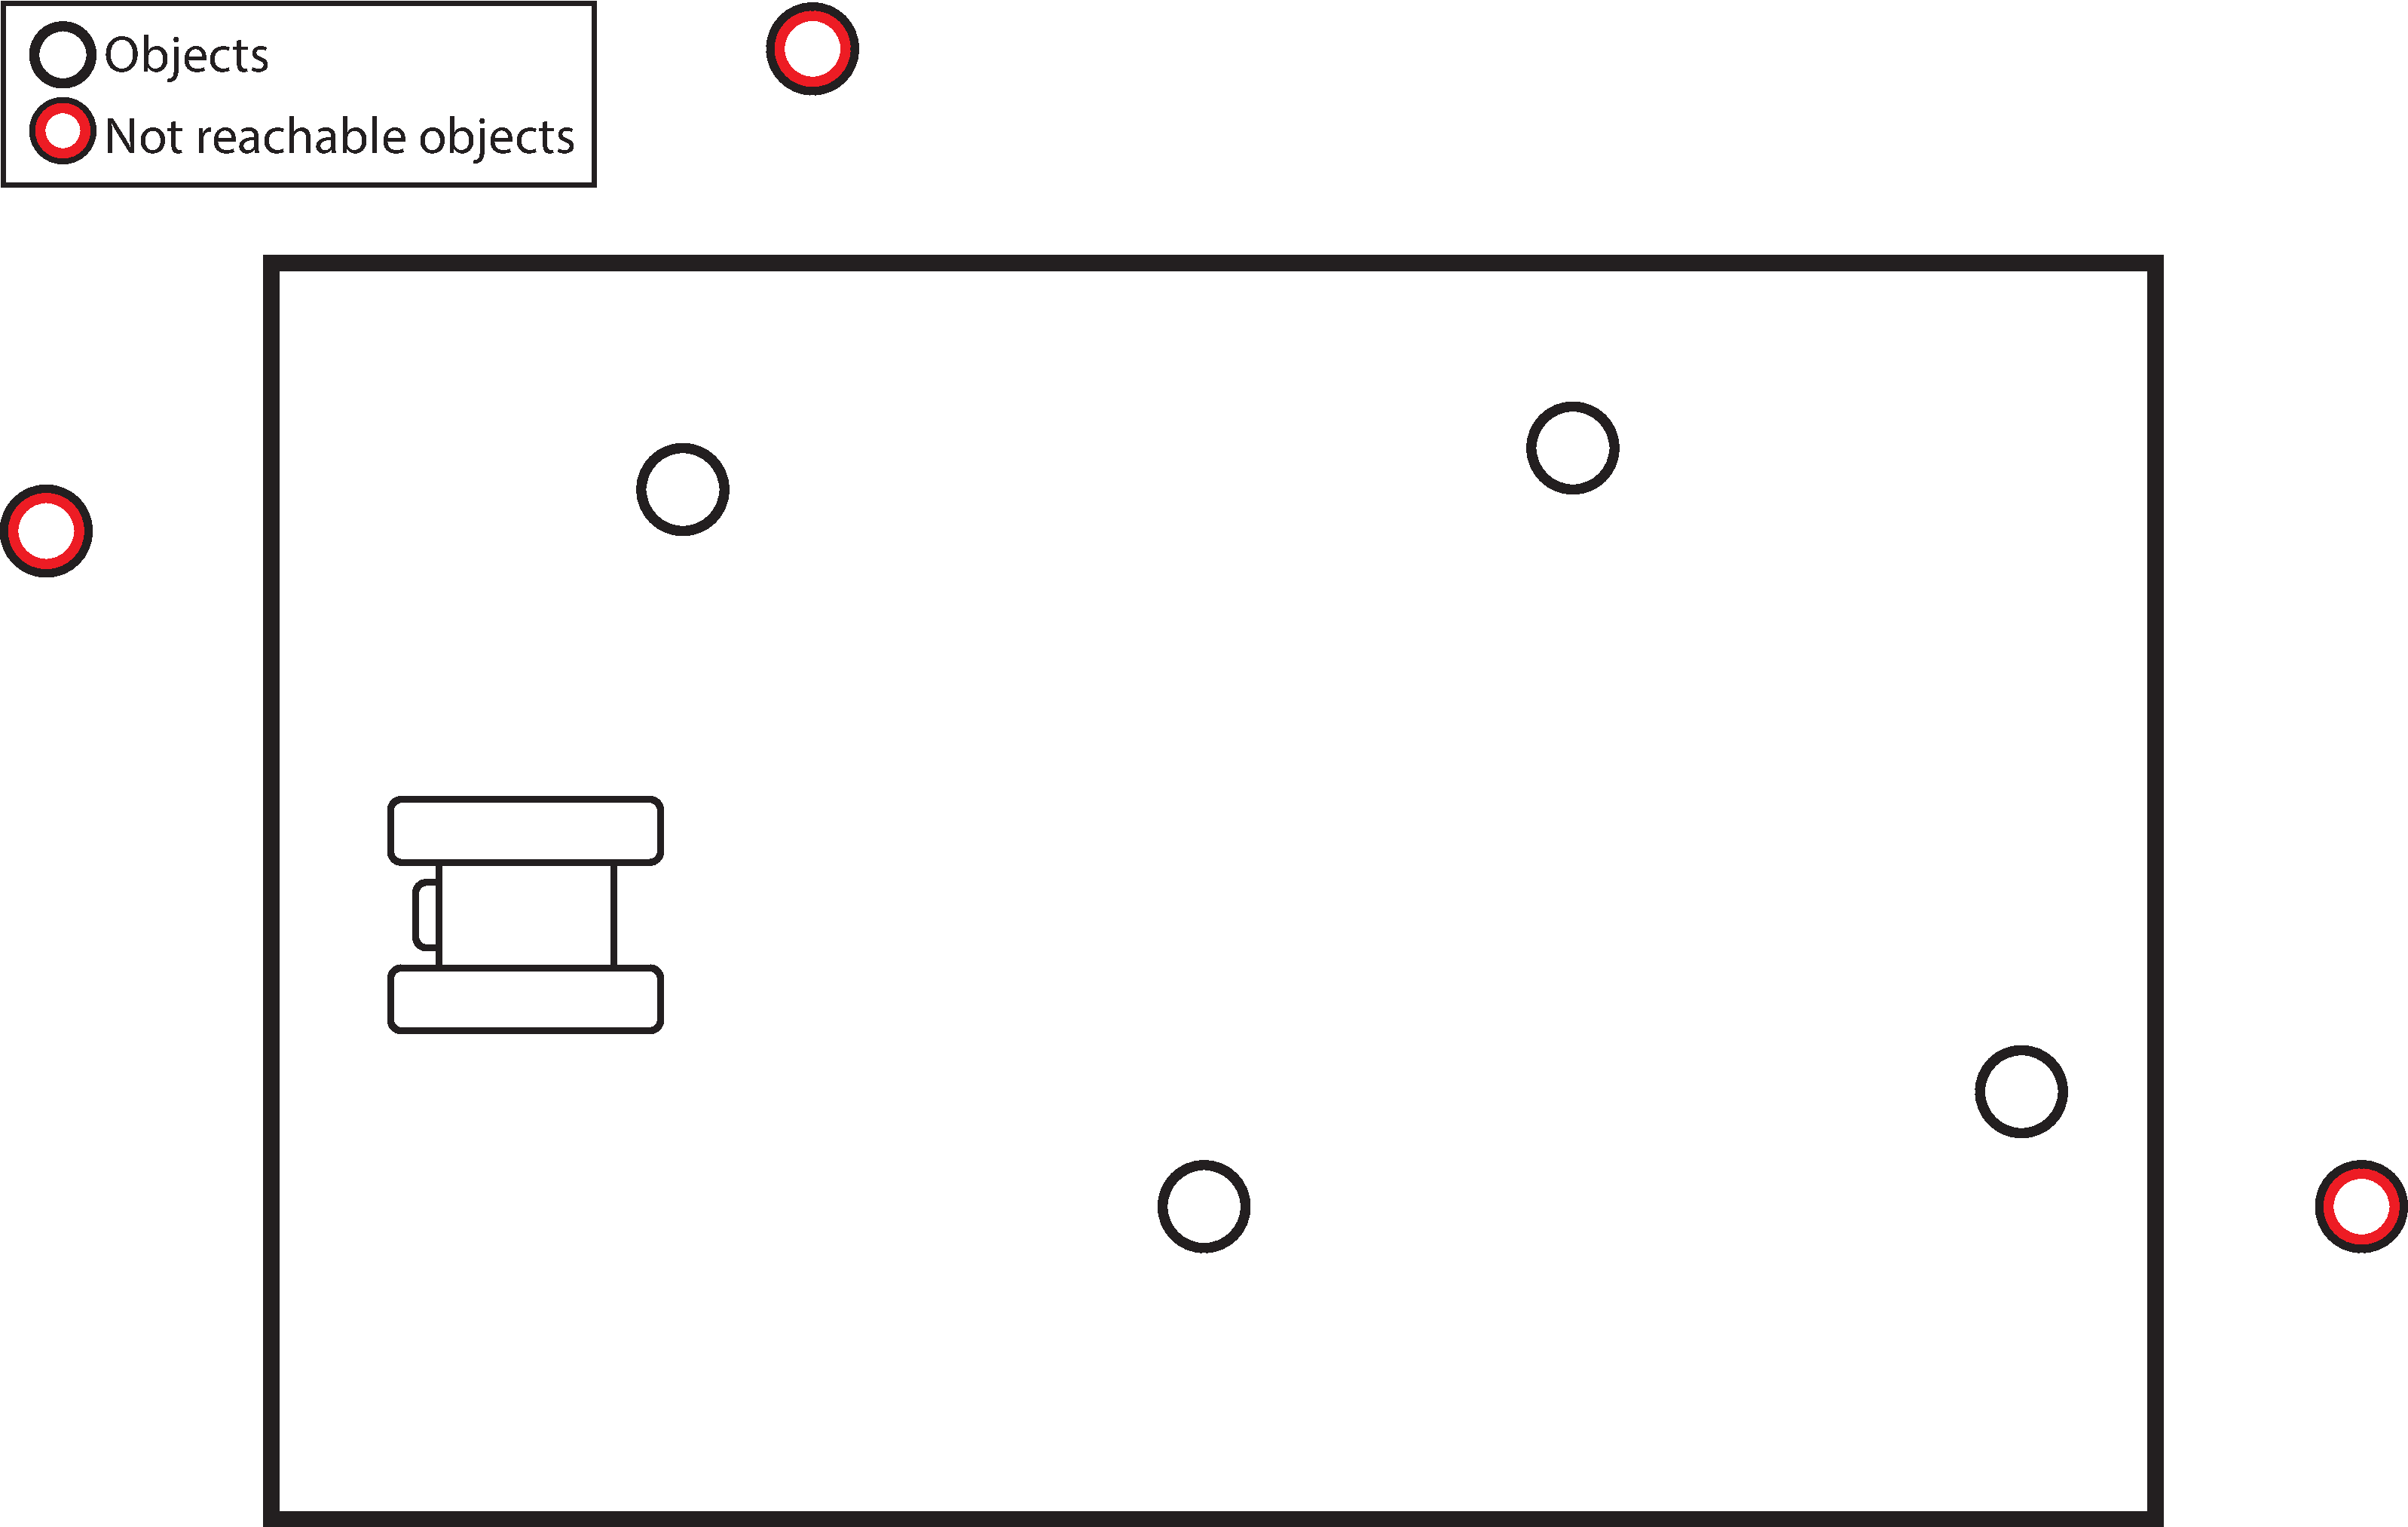
\includegraphics[width=320pt]
     {graphics/TestSetup.pdf}}
     \caption{\label{fig:test-setup} Example of a tested environment.}
\end{figure}

The area was a rectangle with the dimensions 1 m times 1.5 m framed by double layer of black tape. Each test included four cylindrical cans used as objects. Each can had a height of 7 cm, a diameter of 6.5 cm, and a weight of 10 g. An example of a tested environment can be seen in \figref{fig:test-setup}

\section{Results}

All the requirements was tested in one combined test but for each requirement observations were made. The observations for all three requirements is listed below.

\textbf{Navigate the environment within the boundaries}
\begin{itemize}
\item Sometimes the robot does not detects the black lines before its too late.
\item The width of the black lines is important. If the black lines is too thin the robot is less likely detect the boundary.
\end{itemize}

\textbf{Control collection arm to pick up and store objects of specified size}
\begin{itemize}
\item The signal from the slave to the master is not always received when it is finished.
\item Sometimes the robot does not see an object, even if it is right in the front of the robot.
\end{itemize}

\textbf{Find and collect all objects within the time limit}
\begin{itemize}
\item If the distance between the objects is too large, the robot will never find all the objects. 
\item The time used to find objects increases if there is objects on the other side of the black lines.  
\end{itemize}

\begin{table}[H]
	\centering
	\ra{1.3}
  \rowcolors{1}{Gray}{}
   \begin{tabular}{|c|c|c|c|}
   \hline  
   Test no. & Time & Objects & Average time pr. object \\ \hline
      1    & 98.0 seconds    & 4 & 24.5 seconds   \\ \hline
      2    & 98.0 seconds    & 4 & 24.5 seconds  \\ \hline
      3    & 99.0 seconds    & 4 & 24.8 seconds  \\ \hline
      4    & 87.0 seconds    & 4 & 21.8 seconds  \\ \hline
      5    & 108.0 seconds   & 4 & 27.0 seconds  \\ \hline
   \end{tabular}
   \caption{\label{table:FinalTimeTestRobot} Time test of the robot}
\end{table}

In addition to the observations the \tblref{table:FinalTimeTestRobot} shows the time result from the test. The time result is acceptable in relation to the goal from \secref{sec:model}.








% Conclusion
\chapter{Conclusion} \label{cha:evaluation}

% Discussion
\section{Discussion} \label{sec:discussion}

There has been a variety of issues in the implementation of the \projname{}. A lot of these issues have to do with the hardware used for the robot. LEGO NXT was chosen as the platform for the project, because it is a well-established platform for building small robots. The LEGO NXT platform was the available platform provided by the faculty. As a prototype of a larger system, the LEGO NXT is acceptable to use as a platform. However, a number of the sensors are too imprecise and inconsistent for a full scale system.

As seen in \secref{sec:ultrasonic_sensor}, the ultrasonic sensor have a number of issues regarding the tasks it is required to fulfil. It is difficult to distinguish between objects positioned close together and at a distance from the \projname{}. This leads to the \projname{} seeing two objects as one, as seen on \figref{fig:sonar-test-drawing}. Another issue is when an object is close enough to be collected, but the distance measured by the sensor is inaccurate. This results in the \projname{} moving forward towards the object despite already being in grabbing distance. This makes it difficult to determine an object's exact position. It also means that it was difficult mapping the scanned objects relative to each other, as was the case with the NN-algorithm.

A small-step-search was implemented to counter these inaccuracies, when moving towards a found object. As the ultrasonic sensor observes in a cone, it is likely that the objects won't be directly in front of the ultrasonic sensor, and therefore a small-step-search counter this issue. This implementation worked reasonably, but an issue using the small-step-search is that the ultrasonic sensor sometimes won't detect the object and either push it away or drive past it. These issues are due to the ultrasonic sensor's inaccuracy, and occur relatively rarely.

Another issue with the ultrasonic sensor, was that it had trouble detecting objects, that were positioned at certain angles, as described in \secref{sec:ultrasonic_sensor}. When an object is positioned like that, the sound waves will not be reflected back to the sensor, which means that the sensor will not be able to see them. This issue is likely to arise if square objects are used, however using round objects the issue is less likely to occur. A solution to this issue, using the ultrasonic sensor, have not been developed. Using two ultrasonic sensors, to increase precision, was considered, by comparing the results from both sensors. But if these were placed too close to each other, the sensors were going to affect each other. This idea was excluded because of the sensor interference.

The servo motors used for driving the robot also presented issues. This was due to the two motors used, one for each of the tank treads, and because precise movement was desirable, the two motors had to be synchronised. However, the two motors were running differently by default and the robot was not driving straight, which is illustrated in \secref{sec:servo_motor}. This was solved by implementing the motor controller and the speed adjuster, which gave the robot the movement precision it needed.

While the movement worked as intended, there were a lot of trouble with the object detection and thus accurately detecting the objects were difficult. As mentioned previously, the ultrasonic sensor is not precise enough for this task and for the NN-algorithm to work optimally, and a different, more precise sensor is needed. The final version of the \projname{} was meant to use the NN-algorithm to collect the objects, but due to the problems, the next-in-view algorithm was implemented instxead.

%The NN-algorithm requires a lot of precision. Using this algorithm, the robot needs to map the objects in relation to each other and the \projname{}'s starting position. It also needs to keep track of its own position, for example in the case where it hits a black line and have to recalculate its route without needing to scan again. A lot of the precision needed for movement was solved with the motor controller and speed adjuster. The compass sensor also helped ensure that correct angles were given and that the robot could rotate to these angles precisely. Overall the advanced movement for the robot has worked well. A gyro sensor might have been more optimal for this project, since the purpose was to measure rotations and not necessarily magnetic headings, but the compass sensor proved a reasonable replacement.

%It was attempted to make up for some of the inaccuracies by having the robot perform a small-step-search when moving towards a found object. In the world the robot sees that the object is located straight ahead, based on the input from the ultrasonic sensor. However in the actual world the object might be located at the edge of the sensor's cone. Driving straight forward might actually not be the right direction, so when the robot looses the object from it's view, it will perform the small-step-search to correct its angle.

%This has worked reasonably well. The robot does a good job on getting itself back on track and finally picking up the object. This technique relies heavily on the inputs of the ultrasonic sensor. To determine if the object is within the claw and ready to be picked up, the robot considers if the distance returned by the sensor meets a certain requirement. Because of the inaccuracies of the ultrasonic sensor, this has lead to the robot sometimes not detecting that the object is within reach, and have continued driving forward for a little, pushing the object along with it. Another rare case, is when the robot gets close to an object, but drives a little too much forward before correcting its direction. The object will get stuck right outside of the claw and the robot won't be able to collect it.

%Using the ultrasonic sensor, a way to solve this problem has not been found. Depending on the position of the objects and the robot, when the robot is scanning, it is very likely that this situation will arise. However there is no way to predict it. It is not possible to mitigate this inaccuracy, since the objects will not be detected at all. Cylinder-shaped objects like cans are picked up consistently, but the \projname{} is required to be able to pick up objects of different shapes. This is another reason that another, more precise sensor is needed for object detection.

%The project has tried to find a solution to solve the problems regarding the precision of the ultrasonic sensor. A few possible fixes/tweaks to increase the precision were tried: Firstly, the location of the ultrasonic sensor were changed a few times, to find more optimal conditions for the sensor. The result of this were the current location of the ultrasonic sensor, close to the ground and at the chassis of the \projname{}. At an earlier iteration, the sensor had been attached to the claw and this proved not to be a good solution. This also meant that the sensor was closer to the object, but the ultrasonic sensor is imprecise at close distances, as seen in \secref{sec:ultrasonic_sensor}. But the claw is also unstable and might not end at the same position, which might cause problems. The sensor must be as stable as possible. Using two ultrasonic sensors, to increase precision, was also considered, by comparing the results from both sensors. But if these were placed too close to each other, the sensors were going to affect each other. This idea was excluded because of the sensor interference.


% Evaluation
\section{Conclusion} \label{sec:conclusion}

The prototype of the \projname{} was able to fulfil the project goals specified in the problem statement, see \secref{sec:problem_statement}. Staying inside the desired boundary was made possible by utilising two colour sensors. The ultrasonic sensor allows the robot to spot objects while it is moving within the area and determine the distance between these objects and itself. Lastly, the constructed claw along with the ultrasonic sensor were able to determine when an object is within the claws reach, making it able to successfully collect it. 

Most of the hardware were imprecise, but with the used algorithm and the motor controller, the result is sufficient for this prototype. If the \projname{} should be produced for proper usage it would require better hardware, especially to locate objects.



% Future works
\section{Future works} \label{sec:future_works}
This sections presents some of the ideas for future extensions, that could be developed and implemented to make the \projname{} better at collecting objects. 

\subsubsection{Improved object detection}
Having a more precise distance sensor to detect objects would greatly increase the precision while the \projname{} is scanning. Other options could be lasers or cameras.

\subsubsection{Coloured object detection}
Having a colour sensor next to the object detector would allow the robot to determine between object that should be picked up and object that it should ignore. When collecting objects in for example a child's room, there are several objects that the robot should not try to collect such as legs on a table or bed. The robot could be programmed to avoid the colours of these legs. The problem here is that there exist an almost unlimited amount of differently colour table legs, therefore an easier solution would have to be applied. This could for example be to apply a plain-coloured slap bracelet, to each leg with a colour that the robot should ignore \citep{slap_bracelet}.

\subsubsection{Expanded area algorithm}
As it is right now the robot is only able to detect objects that are approximately 50 cm away from it while doing the 360 degrees scan. In a larger room or area this would be far from enough and the robot should therefore be able to more to a new area that has yet to be scanned.

This could be done by driving approximately 100 cm in a chosen direction and do a new search. The problem with this is that the robot might hit an object on the way to the new scanning point. There would also be corners between the circles that the ultrasonic would not have scanned due to the distance.

Another solution would be to drive to the edge of the scanned area and do a new scan from here. This would ensure that no object would be hit while driving to the new area. The problem is that the robot would still do a 360 degrees scan even though that half of the area would already have been scanned. 

A more intelligent solution could be to map the area, while scanning and collecting objects. This would ensure that every position, inside the boundary would be visited, ensuring that all objects inside the boundary are collected. 

\subsubsection{Object deposit area}
While the robot is able to store some objects while driving around, having a deposit area would allow the robot to pick up more objects in a larger area. This would require an exact coordinate system that the robot should be able to follow. This is something that is not implemented in the project, but it was discussed in the early stages as a solution. Being able to find this deposit area and getting back is the primary problem for the robot in its current state. The solution to this would be to place the deposit area at the robots start position, but this would result in a new problem if the robot ever has to do a new 360 degree search. 

\subsubsection{Environment Detection and Colour Calibration}
When detecting the boundaries of the environment, the robot currently checks the floor for any changes in colour. If the robot was to be truly useful in as a non-prototype robot, it would most likely have to detect walls instead of colour on the floor. Both could be useful in different circumstances.

In the finished product, the robot uses hard-coded colour values to check against the input of the colour sensors.. Since black tape was used as a boundary for all tests, it will only be able to detect boundaries of the colour black. To make the robot more dynamic, code was written to allow calibration of the colour sensors: when starting the robot, it would be placed with the sensors above the boundary, and a button would be pressed to calibrate that colour. The same procedure would be repeated for the floor. With two colour variables stored, the robot would be able to calculate an average colour between the two, and ask whether or not the input colour currently seen is more likely to be the boundary or the floor. This code, however, was not implemented in the final product, due to time constraints.



%%%% Kilder %%%%
\begingroup
	\raggedright
	\bibliography{bibliography/literature.bib}
\endgroup
\phantomsection

\addcontentsline{toc}{part}{Appendix}

%%%% Appendiks %%%%
\begingroup
\appendix
\clearforchapter
\phantomsection
% Name \chapter inside the appendices

% Hardware test
\chapter{Hardware Test} \label{app:hardware_test}
This appendix shows the results observed from the performed hardware test.

\section*{Servo motor rotation test} \label{app:servo_motor_test}
This section shows the observed values from the servo motor test. The test is performed according to the description in \secref{sec:servo_motor}. \tblref{table:app_motor_test} shows the raw rotation values collected from the test, as well as the difference between the two motors. 

\begin{table}[H]
	\centering
	\ra{1.3}
	\rowcolors{1}{Gray}{}
    \begin{tabular}{lccc}
    \hline  
    \rowcolor{DGray}
    \textbf{Power Level}~~~~~~~~~~~~ & Motor L(Degrees) & Motor R(Degrees) & Difference \\ \hline 
    100\%                  & 6,658                  & 6,666                & 0,12\% \\
    90\%                   & 5,823                  & 5,912                & 1,51\% \\
    80\%                   & 5,192                  & 5,262                & 1,33\% \\
    70\%                   & 4,495                  & 4,571                & 1,67\% \\
    60\%                   & 3,859                  & 3,923                & 1,64\% \\
    50\%                   & 3,145                  & 3,211                & 2,07\% \\
    40\%                   & 2,479                  & 2,551                & 2,86\% \\
    \hline  
    \end{tabular}
    \caption{\label{table:app_motor_test}Servo motor test of rotations.}
\end{table}

\newpage
\section*{Ultrasonic sensor distance test} \label{app:ultrasonic_sensor_test}
This section shows the observed values from the ultrasonic sensor distance test. \secref{sec:ultrasonic_sensor} describes the testing method. \tblref{table:app_ultrasonic_sensor_test} shows the observed sensor values, called value, and the actual distance. The difference between the values is also shown. 

\begin{table}[H]
	\centering
	\ra{1.3}
	\rowcolors{1}{Gray}{}
    \begin{tabular}{|lcc|lcc|}
    \hline  
    \rowcolor{DGray}
    \textbf{Actual distance} & \textbf{Value}  & \textbf{Difference} &\textbf{Actual distance} & \textbf{Value}  & \textbf{Difference}\\ \hline
    1 cm     & 8 cm     & 700\%  &    13 cm     & 16 cm     & 23\% \\
    2 cm     & 7 cm     & 250\%  &    14 cm     & 16 cm     & 14,2\% \\
    3 cm     & 6 cm     & 100\%  &    15 cm     & 17 cm     & 13,3\% \\
    4 cm     & 7 cm     & 75\%   &    20 cm     & 20 cm     & 0\% \\
    5 cm     & 7 cm     & 40\%   &    25 cm     & 25 cm     & 0\% \\
    6 cm     & 7 cm     & 16,6\% &    30 cm     & 32 cm     & 6,6\% \\
    7 cm     & 8 cm     & 14,2\% &    40 cm     & 41 cm     & 2,5\% \\
    8 cm     & 10 cm    & 25\%   &    50 cm     & 51 cm     & 2\% \\
    9 cm     & 11 cm    & 22,2\% &    100 cm    & 101 cm    & 1\% \\
    10 cm    & 13 cm    & 30\%   &    150 cm    & 150 cm    & 0\% \\
    11 cm    & 14 cm    & 27,2\% &    200 cm    & 255 cm    & 27,5\% \\
    12 cm    & 15 cm    & 25\%   &              &           &\\
    \hline 
    \end{tabular}
    \caption{\label{table:app_ultrasonic_sensor_test} Ultrasonic Sensor test at distances.}
\end{table}


\newpage
\section*{Ultrasonic rotation test graph} \label{app:sonar-test-graph}
This section shows the observations from the ultrasonic sensor rotation test plotted into a graph. Every time the values goes down, a new object has been spotted. There were placed five objects in this test.

The objects were placed at the following degrees:
\begin{description}
\item[Object 1] 0 degrees
\item[Object 2] 90 degrees
\item[Object 3] 180 degrees
\item[Object 4] 225 degrees
\item[Object 5] 270 degrees
\end{description}

\begin{figure}[H]
     \center{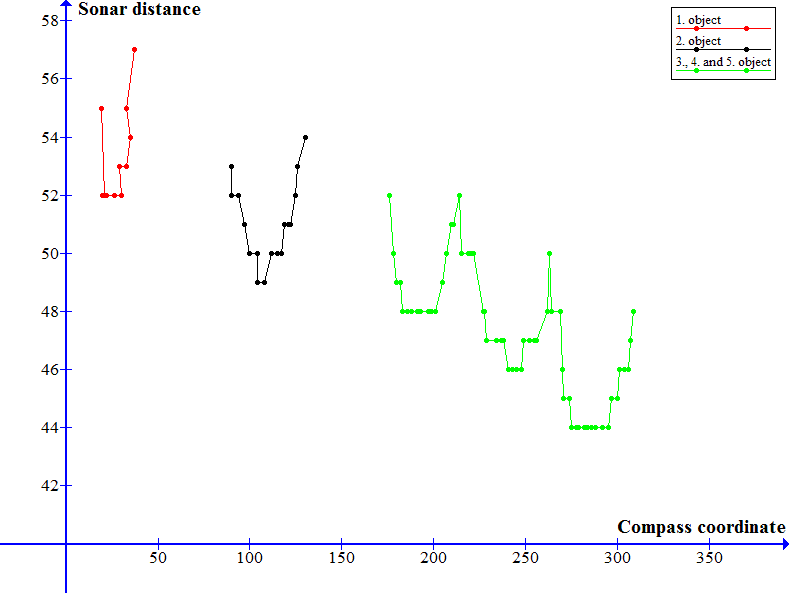
\includegraphics[width=\textwidth]
     {graphics/ObjectSpotting2.png}}
     \caption{\label{fig:sonar-test-graph} 360 degree test with ultrasonic sensor.}
\end{figure}

As seen in \figref{fig:sonar-test-graph}, if the objects are placed close together, the objects can not be distinguished from each other, resulting in object number 3., 4., and 5. counting as one big object. 









% Sequence diagram
%\chapter{Sequence diagram} \label{app:sequence-diagram}
This appendix shows a sequence diagram of the first iteration.

\begin{figure}[H]
     \center{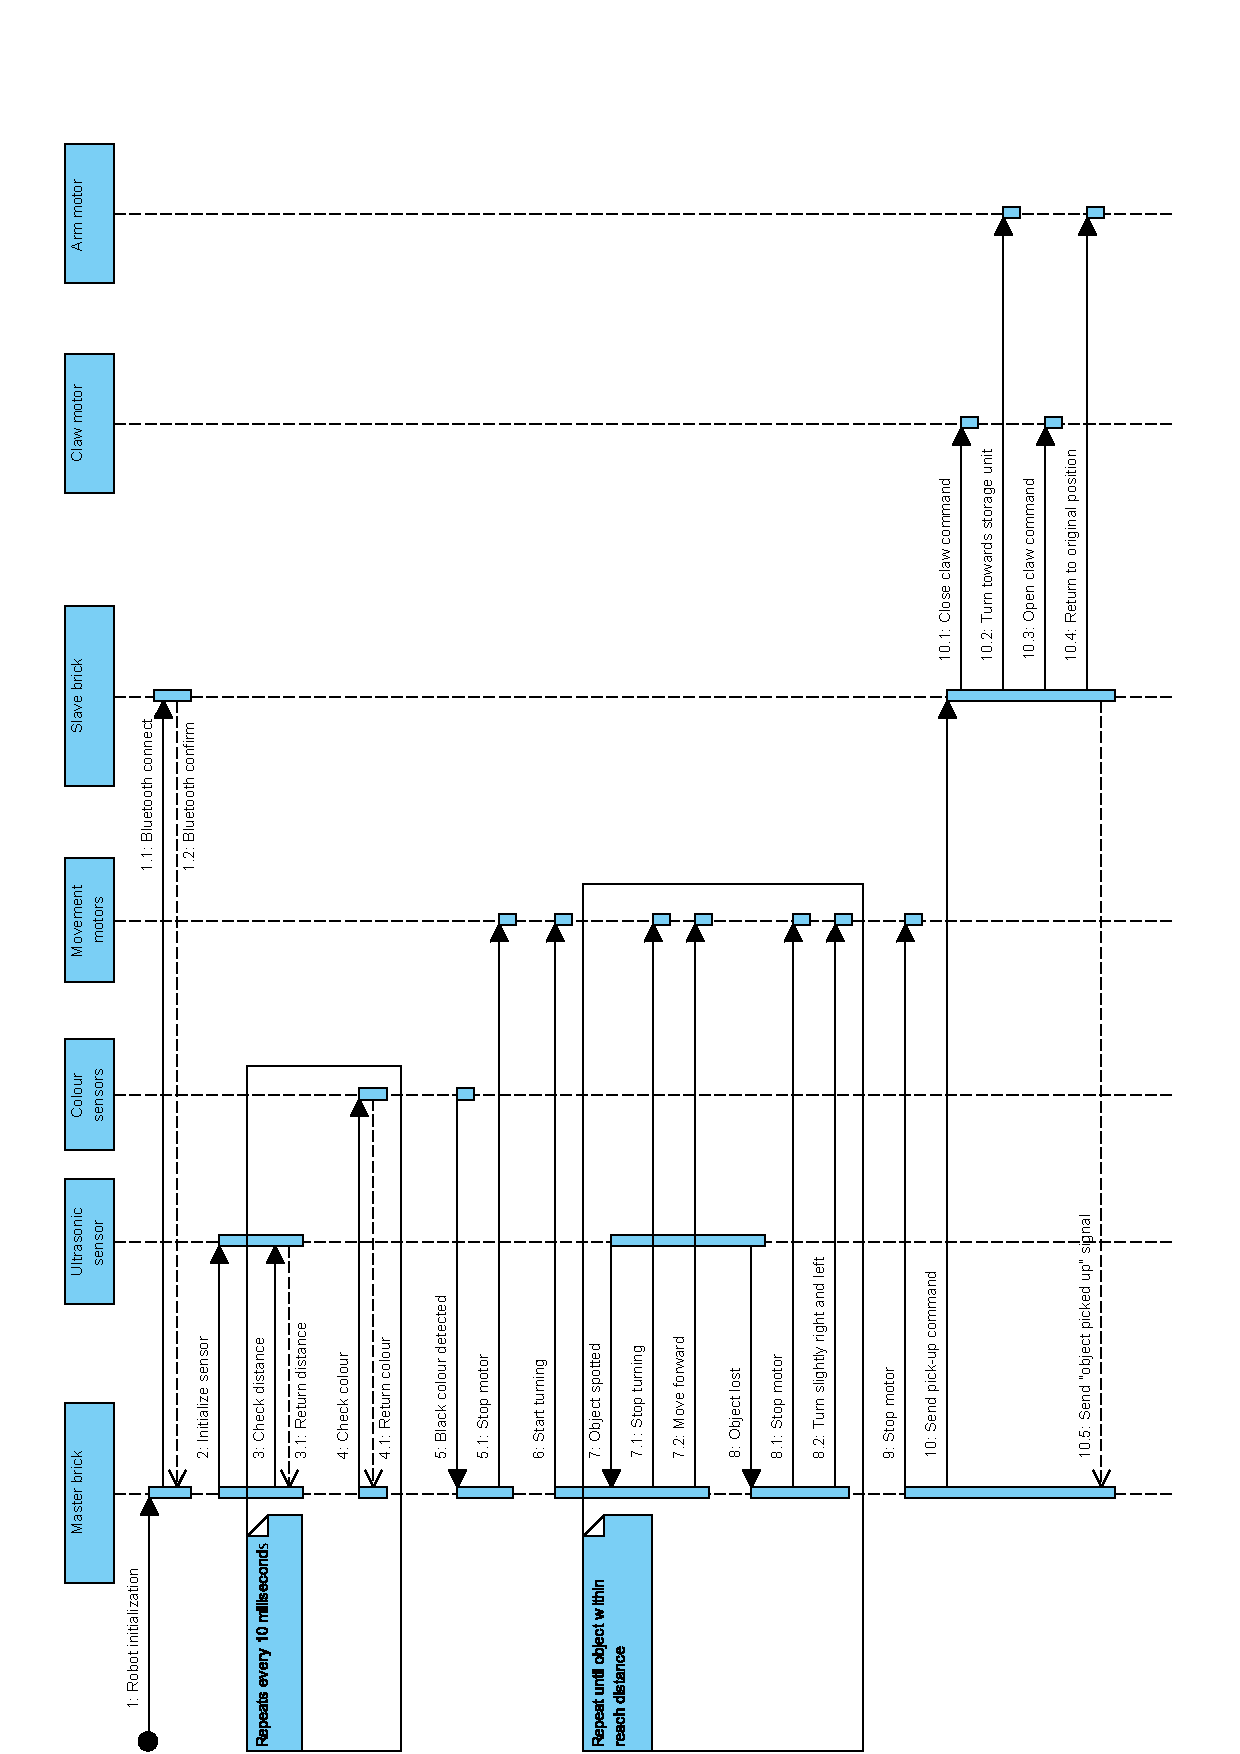
\includegraphics[width=\textwidth]
     {graphics/SequenceDiagram.pdf}}
     \caption{\label{fig:sequence-diagram-appendix} First iteration }
\end{figure}





% cd
\chapter{CD} \label{app:CD}


\begin{enumerate}
\item Source code for final master
\begin{itemize}
\item /Program/Master/Master.cpp
\item /Program/Master/Master.oil 
\item /Program/Master/Makefile
\end{itemize}
\item Source code for final slave
\begin{itemize}
\item /Program/Slave/Slave.cpp
\item /Program/Slave/Slave.oil
\item /Program/Slave/Makefile
\end{itemize}
\item Source code using nearest neighbour algorithm
\begin{itemize}
\item /Algorithm/Master/MasterNN.cpp
\item /Algorithm/Master/MasterNN/MasterNN.oil
\item /Algorithm/Master/Makefile
\end{itemize}
\item Report
\begin{itemize}
\item /Report/Report.pdf
\end{itemize}
\end{enumerate}


\endgroup

%%%% Fixme/fxnotes %%%%
%\listoffixmes

\end{document}


%%%% Skabelon til et billede %%%%
%\begin{figure}[H]
%     \center{\includegraphics[width=\textwidth]
%     {graphics/Billedenavn.pdf}}
%     \caption{\label{fig:Billedenavn} Billede tekst.}
%\end{figure}

%%%% Skabelon til en lstlisting %%%%
%\begin{lstlisting}[caption= Look at my fancy \lstref{lst:testlst}, label=lst:testlst]
%...
%\end{lstlisting}

%%%% Skabelon til en tabel %%%%
%\begin{table}[H]
%	\centering
%	\ra{1.3}
%   \rowcolors{1}{Gray}{}
%   \begin{tabular}{lcc}
%   \hline  
%   Tekst    & Mere tekst    & Endnu mere tekst  \\ \hline  \rowcolor{Gray}
%   Tekst    & Mere tekst    & Endnu mere tekst  \\ 
    %Copy the two lines if more is needed.
%   \hline 
%   \end{tabular}
%   \caption{\label{table:TableNameForReferencing} Table tekst.}
%\end{table}